  \documentclass[12pt]{report}
%\usepackage{helvet}
%\renewcommand{\familydefault}{\sfdefault}

\usepackage[latin1]{inputenc}
\usepackage[T1]{fontenc}
%https://www.teuderun.de/latex/layout/microtype-paket/
\usepackage{microtype}
%zur Benutzung von Grafiken
%\usepackage{graphicx}
\usepackage[draft]{graphicx} %aktivieren f�r schnelleren Typeset
%f�r Kapitelformatierung
\usepackage{titlesec}
%f�r Zeilenabstand
\usepackage{setspace}
%f�r Deutsche Bezeichungen wie "Tabellenverzeichnis"
\usepackage[ngerman]{babel}
\selectlanguage{ngerman}
%Seitenlayout
\usepackage[a4paper,top=20mm,bottom=20mm,left=30mm,right=30mm]{geometry}
%Bib-Ressourcen erm�glichen, Stil setzen und genau parametrieren
\usepackage[idembib=false,
style=footnote-dw,
natbib=true,
edsuper=true,
nopublisher=false,
urldate=long,
hyperref,
backend=biber,
maxcitenames=2,
maxbibnames=99,
doi=true,
isbn=true
]{biblatex}
\AtEveryCitekey{\clearfield{isbn}}
\AtEveryCitekey{\clearfield{issn}}
\AtEveryCitekey{\clearfield{doi}}
%Titel kursivieren
\DeclareFieldFormat{title}{\mkbibemph{#1}}
\DeclareFieldFormat{citetitle}{\mkbibemph{#1}}
%in ingerman "andothers", was zu u. a. f�hrt, durch et al. ersetzen
\DefineBibliographyStrings{ngerman}{
   andothers = {{et\,al\adddot}},
}
%Autoren in der Bibliography als Nachname, Vorname
\DeclareNameAlias{sortname}{family-given}
\renewcommand*{\multinamedelim}{\addcomma\space}
\renewcommand*{\finalnamedelim}{\addcomma\space}
\renewcommand*{\nameyeardelim}{\addcomma\space}
\setlength{\bibitemsep}{0.35\baselineskip}
%\renewbibmacro{in:}{}
%\DefineBibliographyStrings{ngerman}{u. a.={et al.\hspace{1mm}}}
%F�r das Abk�rzungsverzeichnis alternativ: \usepackage[toc]{glossaries}
\usepackage[acronym,nonumberlist,automake]{glossaries}
%f�r diagonal geteilte Zellen in Tabellen, Befehl ist \backslashbox{}
\usepackage{diagbox}
%Ben�tigt, um Tabellen automatisch am Rand umzubrechen
\usepackage{tabularx,ragged2e}
\usepackage{makecell}
%Ben�tigt, um Captions bei Tabellen jeweils zu zentrieren, k�nnte auch in den Metadaten f�r alle passieren
\usepackage{caption}
%F�r ToDo-Annotationen, bei Bedarf entfernen
\usepackage{todonotes}
%klickbare �berschriften und Co.
\usepackage{hyperref}

%ben�tigt, um Abbildungen im Anhang nicht in den Verzeichnissen zu haben.
\usepackage{ifthen}

%Bef�llen f�r Abk�rzungen
\newacronym{TOGAF}{TOGAF}{The Open Group Architecture Framework}
\newacronym{PK}{PK}{Planung und Kontrolle}
\newacronym{IV}{IV}{Informationsversorgung}
\newacronym{F+E}{F\&E}{Forschung und Entwicklung}
\newacronym{KuE-C}{KuE-C}{Kosten- und Erfolgscontrolling}
\newacronym{F-C}{F-C}{Finanzcontrolling}
\newacronym{I-C}{F-C}{Investitionscontrolling}
\newacronym{R-C}{R-C}{Risikocontrolling}
\newacronym{B-C}{B-C}{Beschaffungscontrolling}
\newacronym{P-C}{P-C}{Produktionscontrolling}
\newacronym{M-C}{M-C}{Marketingcontrolling}
\newacronym{L-C}{L-C}{Logistikcontrolling}
\newacronym{Pr-C}{Pr-C}{Projektcontrolling}
\newacronym{H-C}{H-C}{Hochschulcontrolling}
\newacronym{Per-C}{Per-C}{Personalcontrolling}
\newacronym{V-C}{V-C}{Vertriebscontrolling}
\newacronym{JIT-L}{JIT-L}{Just-In-Time-Lieferung}
\newacronym{KLR}{KLR}{Kosten- und Leistungsrechnung}
\newacronym{PMBOK}{PMBOK}{Project Management Body of Knowledge}
\newacronym{ROI}{ROI}{Return-On-Investment}
\glsaddall
%Parametrierung der Packages
%section als 1 statt 1.1, damit Chapter nicht ben�tigt wird
\renewcommand{\thesection}{\arabic{section}}

%auch ab Ebene 3 bis 5 nummerieren
\setcounter{secnumdepth}{5}

%Stil der Kopf- und Fu�zeilen
\newpagestyle{mainmatter}{%
  \setheadrule{1pt}
  \sethead{\thesection ~\sectiontitle}{}{\thesubsection ~\subsectiontitle}%
  \setfoot{}{\thepage}{}
}
\newpagestyle{rest}{%
  \sethead{}{}{}
  \setfoot{}{\thepage}{}
}
%damit auch der Name der Subsection erkannt wird
\settitlemarks{section,subsection,subsubsection}



%Bilder in Unterordner suchen
\graphicspath{{image/}}

%Zeilenabstand
\setstretch{1.5}

%Bib-Ressourcen einbinden
\addbibresource{bibliography.bib}

%Tiefe des Inhaltsverzeichnisses
\setcounter{tocdepth}{3}

%neue Seite nach Kapitelende
\newcommand{\sectionbreak}{\clearpage}


%URLs im Literaturverzeichnis umbrechen
\setcounter{biburllcpenalty}{7000}
\setcounter{biburlucpenalty}{8000}

%Fu�zeilen nicht auf n�chster Seite fortf�hren
\interfootnotelinepenalty=10000

%Kurzreferenz bei zweiter Benutzung ohne "wie Anm. x"
\renewcommand\citenamepunct{\addcomma\space}
\renewbibmacro*{cite:seenote}{}

%Vertikale Zentrierung von Zelleninhalten
\renewcommand\tabularxcolumn[1]{m{#1}}
\newcolumntype{C}{>{\Centering\arraybackslash}X} % centered "X" column
\newcolumntype{L}{>{\raggedleft\arraybackslash}X} % centered "X" column
\newcolumntype{R}{>{\raggedright\arraybackslash}X} % centered "X" column

%Fu�noten kleiner machen
\renewcommand{\footnotesize}{\scriptsize}

%Enumerates in Enumerates erm�glichen also 1., 2., 2.1., 2.2., 3., etc.
%\renewcommand{\labelenumii}{\theenumii}
%\renewcommand{\theenumii}{\theenumi.\arabic{enumii}.}

%mit \tocless sections erzeugen, die nicht im toc auftauchen
\newcommand{\nocontentsline}[3]{}
\newcommand{\tocless}[2]{\bgroup\let\addcontentsline=\nocontentsline#1{#2}\egroup}


\tikzset{
  basic/.style  = {draw, text width=2.5cm, drop shadow, font=\sffamily, rectangle},
  root/.style   = {basic, rounded corners=2pt, thin, align=center,
                   fill=green!30},
  level 2/.style = {basic, rounded corners=6pt, thin,align=center, fill=green!60,
                   text width=8em},
  level 3/.style = {basic, thin, align=left, fill=pink!60, text width=6.5em}
}

%engeres itemize
\newenvironment{tightenumerate}{
\begin{enumerate}{
\setlength{\topsep}{-1ex}
\setlength{\itemsep}{-1ex}
\setlength{\leftmargin}{4ex}
}
}{
\end{enumerate}
\vspace{1ex}
}

%Seitennummerierungen
\newcounter{savepage}
\def\frontmatter{
	\pagestyle{rest}
    \pagenumbering{Roman}
    \setcounter{page}{1}
}

\def\mainmatter{
	\pagestyle{mainmatter}
	\setcounter{savepage}{\number\value{page}}
	\newpage
	\pagenumbering{arabic}
}

\def\backmatter{
	\pagestyle{rest}
  	\newpage
	\pagenumbering{Roman}
	\setcounter{page}{\value{savepage}}
}
%Zeilenumbr�che f�r W�rter, die Latex nicht kennt
\hyphenation{Be-r�ck-sich-ti-gung}
\hyphenation{�n-der-ungs-ver-ur-sach-ten}
\hyphenation{Ur-sa-che-Wir-kungs-Zu-sam-men-h�n-gen}
\hyphenation{Ein-schicht-Voll-zeit-t�-tig-keit}

%Latex Smartdiagram, B�umc zeichnen und Stil
\usepackage{forest}
\useforestlibrary{edges}

%footnote ohne Indent
\usepackage[hang,flushmargin,bottom]{footmisc}

%Tabelle �ber mehrere Seiten in diesem environment
\usepackage{longtable} 

\usepackage{array}

%itemizes nebeneinander
\usepackage{varwidth}

%mit [H] figures und tables festnageln
\usepackage{float}

%f�r \setlist{nolistsep}
\usepackage{enumitem}

%f�r Formeln
\usepackage{amsmath}

%Anhang nicht im TOC
\usepackage{etoolbox}
\appto\appendix{\addtocontents{toc}{\protect\setcounter{tocdepth}{1}}}
\appto\listoffigures{\addtocontents{lof}{\protect\setcounter{tocdepth}{1}}}
\appto\listoftables{\addtocontents{lot}{\protect\setcounter{tocdepth}{1}}}

%Abk�rzungsverzeichnis erstellen
\makeglossaries
%\makeindex
\begin{document}
\frontmatter
%\title{
%{Thesis Title}\\
%{\large Nordakademie Graduate School}\\
%{
\includegraphics{nak.jpg}}
%}
%\author{Sebastian Schack}
%\date{17.04.2019}
%
%\maketitle


\thispagestyle{empty}
\vspace{2cm}
\begin{center}

\includegraphics[width=0.85\textwidth]{nak} 
\\\vspace{2cm}

\Large{Konzeptioneller Beitrag zur Bewertung von Flexibilit�t als Werttreiber in der gesch�ftlichen IT}

\vspace{1cm}
\large{Masterarbeit}

\vspace{5mm}
\large{Wirtschaftsinformatik $|$
 NORDAKADEMIE}
\vspace{1	cm}
\end{center}
{\large
\begin{flushleft}
%\linespread{3}
\textbf{Vorgelegt von:} Sebastian Schack \\
\textbf{Geboren am:} 29.10.1991\\
\textbf{Matr.-Nr.:} 9018 \\
\textbf{Gutachter:} \\
\begin{tightlist}
	\item \hspace{1cm} Prof. Dr. Hinrich Schr�der
	\item \hspace{1cm} Prof. Dr. Michael Schulz\\
\end{tightlist}
\vspace{5mm}
\textbf{Abgabe:} \today\\
\end{flushleft}
}
\vspace{1cm}

\newpage

\tableofcontents 
\newpage
\addcontentsline{toc}{section}{Abbildungsverzeichnis}
\listoffigures
\newpage
\addcontentsline{toc}{section}{Tabellenverzeichnisverzeichnis}
\listoftables
\newpage
%\addcontentsline{toc}{section}{Abk�rzungsverzeichnis}
\printglossary[type=\acronymtype,title=Abk�rzungsverzeichnis]

\newpage
\mainmatter
\section{Einleitung}
\subsection{Motivation und Zielsetzung}
Steigende Durchdringung unternehmerischen Umfelds durch informationstechnologische Systeme und die damit einhergehende steigende Gr\"o{\ss}e von IT-Organisationen, die unterst\"utzend oder direkt wertsch\"opfend die IT-Services zur Verf\"ugung stellen, zwingen IT-Verantwortliche, M\"oglichkeiten zur objektiven und zielgerichteten Steuerung der Gesamt-IT-Organisation zu etablieren.\newline
Der Ansatz des Controllings, zentrale Aufgaben des Managements mittels dementsprechender Methoden aufeinander abzustimmen, soda{\ss} bestm\"ogliche Rahmenbedingungen zur unternehmerischen Zielerreichung geschaffen werden, ist lange etabliert.\footnote{Vgl. z.B. \cite[S.176f]{woehe2016einfuehrung} sowie \cite[S.25]{Horvath2015} und \cite[S.33ff]{kuepper2013controlling}, au{\ss}erdem \cite[S.20ff]{weber2015einfuehrung} zu anderen Definitionsans\"atzen}\newline
Der Einsatz von Information{\ss}ystemen war fr\"uher prim\"ar technisch orientiert.\footnote{Vgl. \cite[S.VII]{Gadatsch2014}}\newline
Seit etwa 1990 verdichtet sich bei IT-Verantwortlichen allerdings die Ansicht, da{\ss} diese Systeme als Produktionsfaktor mit dem Controlling-Ansatz zu vernetzen sind.\footnote{Vgl. \cite[S.VII]{Gadatsch2014}}
Viele Elemente des kla{\ss}ischen Finanzcontrollings oder anderer Teilbereiche, wie z.B. die Balanced Scorecard, sind auch im IT-Controlling bereits gel\"aufig und k\"onnen anhand bestehender Methoden darauf ausgerichtet werden.\footnote{Vgl. \cite[S.46]{kesten2013}}\newline
Die Rolle der IT-Organisation in einem Unternehmen kann verschieden ausgelegt werden, da die in der Praxis vorzufindenden Konstrukte durch die M\"oglichkeiten externer Dienstleister sowie Technologieanbieter (z.B. Cloud-Dienste) Schwerpunkte setzen m\"u{\ss}en.\footnote{Vgl. \cite[S.581f]{schroederHMD2016}}\newline
In der Folge wird h\"aufig nicht die Gesamtheit einer theoretisch durch eine IT-Abteilung abdeckbaren T\"atigkeiten tats\"achlich erbracht , sondern basierend auf inneren und \"au{\ss}eren Einfl\"u{\ss}en Verantwortlichkeitsverteilung vorgenommen.\footnote{Vgl. \cite[S.585-590]{schroederHMD2016}}\newline
Die in diesem Kontext notwendige Flexibilit\"at, die dazu dienen kann, mit IT-Organisationen auf z.B. organisatorische Ver\"anderungen oder technologische Schwierigkeiten zu reagieren, um sie trotz kontinuierlich komplexer werdenden Umfelds zielsicher steuern zu k\"onnen und innerhalb dieser Rahmenbedingungen \"okonomisch bestm\"ogliche Verh\"altni{\ss}e zu erreichen, ist bisher nicht Bestandteil einer integrierten Betrachtung des IT-Controllings.\newline
Auch dedizierte bzw. isolierte Untersuchungen zu Flexibilit\"atsaspekten existieren nur wenig und veraltet\footnote{Vgl. z.B. die fast 20 Jahre alten Beitr\"age \cite[S.168ff]{byrdturner2000} und \cite[S.21ff]{byrdturner2001}}, ber\"ucksichtigen also nicht die aktuell vorherrschenden Zust\"ande.
Diese f\"ur die IT ausgebliebene Betrachtung von Flexibilit\"at ist allerdings fester Bestandteil des Produktionscontrollings und und dort wird sie auch als konkreter Wertbeitrag verstanden.\footnote{Vgl. \cite[S.8f]{Gottmann2019}}
Angesichts beschriebener Umst\"ande, auf die auch produzierendes Gewerbe (im Sinne der produzierenden Abteilungen) reagieren m\"u{\ss}en, ist Flexibilit\"at als wertsch\"opfender Aspekt auch in informationstechnologischer Hinsicht wahrscheinlich.
Diesen zu definieren, in Anlehnung an andere Teilbereiche des Controllings me{\ss}bar zu machen und zu interpretieren ist Ziel und Bestandteil dieser Arbeit.

\subsection{Forschungsrelevanz}
Das Feld der unternehmerisch genutzten Informationstechnologie ist dynamisch und kurzweilig - ein Charakteristikum, de{\ss}en Auspr\"agung sich bis heute versch\"arft.\footnote{Vgl. \cite[S.15]{capgemini2019}} 
Daher ist nicht verwunderlich, da{\ss} nationale und internationale Studien unabh\"angig voneinander immer wieder darauf hindeuten, dass IT-Projekte scheitern oder zumindest nicht erwartungskonform verlaufen.\footnote{Vgl. \cite[S.172]{fischer2016}}\newline
Ein zu verzeichnender Trend ist zum Beispiel, da{\ss} Projektmanagement-Methoden tendenziell h\"aufiger agil als plangetrieben ausgelegt werden\footnote{Vgl. \cite[S.12]{statusquoagile2015}} und dadurch subjektiv be{\ss}ere Resultate erzielt werden.\footnote{Vgl. \cite[S.22]{statusquoagile2015}} 
Es l\"a{\ss}t sich f\"ur Projekte ein Flexibilisierungstrend erkennen.\newline
Was bedeutet Flexibilit\"at nun aber f\"ur die Gesamtauslegung der IT-Organisation?
Potentiellen Erwartungen steht gegen\"uber, da{\ss} dedizierte Auseinandersetzung bis vor zehn Jahren weder wi{\ss}enschaftlich noch praktisch stattfand.\footnote{Vgl. \cite[S.53]{radermacher2009}} 
Nichtsdestotrotz erkannten bereits 2008 - also in laut einer Studie der Capgemini Unternehmensvertreter, da{\ss} IT-Flexibilisierung als ``Megatrend'' einzustufen ist und Grund f\"ur ``fundamentale Transformationsprozesse'' sein wird.\footnote{Vgl. \cite[S.17]{capgemini2008}}
Ratzer fa{\ss}t die Relevanz von Flexibilit\"at wie folgt zusammen: ``Um diese Situation be{\ss}er kontrollieren zu k\"onnen, wird im Gegenzug eine noch weiter entwickelte IT ben\"otigt, die wiederum erneut den Komplexit\"ats- und Unsicherheitsgrad des Wettbewerbsumfelds erh\"oht. 
Dieser Mechanismus voll- zieht sich in immer k\"urzeren Ver\"anderungszyklen, denen sich IT-Organisationen anpa{\ss}en m\"u{\ss}en. 
Eine deutliche h\"ohere Flexibilit\"at ist n\"otig.''\footnote{\cite{ratzer2009}}
Auch Wiedenhofer sieht in der Dynamik die Notwendigkeit f\"ur Flexibilit\"at gegeben, um damit auf auftretende Probleme zu reagieren: ``Durch die Schaffung von geeigneten Strukturen steigert die IT-Organisation ihre Handlungsflexibilit\"at. 
Mit dieser F\"ahigkeit kann sie schnell auf wechselnde und komplexe Anforderungen reagieren.''\footnote{\cite[S.236]{Wiedenhofer2016}}
Er sieht in k\"urzeren Innovationszyklen, steigender Digitalisierung und der Geschwindigkeit des konjunkturellen Wandels insbesondere eine Bedrohung f\"ur bestehende Gesch\"aftsmodelle\footnote{Vgl. \cite[S.237]{Wiedenhofer2016}}, auf die mit Flexibilit\"at zu reagieren ist.\newline
Zwar ist die Dynamik- bzw. Komplexit\"atsfloskel eine repetitiv paraphrasierte Scheinbegr\"undung, doch ist zu ermitteln, da{\ss} sich die Kontextualisierung der Forderung nach Flexibilit\"at mit dieser Art als problematisch eingestuften Rahmenbedingungen selbst in wi{\ss}enschaftlichen Beitr\"agen bis heute erhalten hat, soda{\ss} diesbez\"ugliche Relevanz tats\"achlich im Zusammenspiel beider Seiten zu begr\"unden ist. 
Tats\"achlich ist die Relevanz hinsichtlich praktischer Forschung weiter auch damit zu begr\"unden, da{\ss} die Behandlung zwar in der Fachwelt erfolgt, konkrete, konsensf\"ahige Beurteilungsmethoden und Handlungsvorschl\"age, z.B. auf Basis von Szenarioeinordnungen aber nicht ihren Weg in einschl\"agige Publikationen (z.B. Gadatsch, Mayer oder Tiemeyer) gefunden haben.


\subsection{Methodisches Vorgehen}
%Analogiemethode
Ziel der Arbeit ist, wie in Kapitel 3 angesprochen, Me{\ss}barkeit von Flexibilit\"at zu untersuchen und ein Rahmenwerk zu definieren, welches Methoden aus dem Produktionscontrolling ableitet und zu eruierenden Zielen und Zwecken zuf\"uhrt, welche wiederum aus allgemeinen Anspru\"uchen des Controllings abzuleiten sind. Auf diesem Weg soll Flexibilita\"at als Wertreiber greifbar und verst\"andlich werden, also auch verdeutlicht werden, welcher Nutzen aus flexiblen IT-Architekturen gezogen werden kann.
Ziel ist allerdings nicht, Flexibilit\"at an konkreten Beispielen zu me{\ss}en und den Wertsch\"pfungsbeitrag zu analysieren.
Grundlage der Forschung ist daher die theoretische, also auf Literatur gest\"utzte Erarbeitung von Grundlagen und Zielen des Controllings, Implementationsweisen und Zielen im Produktionscontrolling, werttreibenden Aspekten unternehmerischer IT, Auswirkungen von ausreichender und mangelnder Flexibilita\"at, Aufbau von Rahmenwerken des IT-Controllings und letztlich die integrierte Konsolidierung in einem Rahmenwerk zur Me{\ss}ung f\"ur das IT-Controlling. 
Dieses Vorhaben hat deduktiven Charakter, wobei allerdings nicht vom ``Allgemeinen auf einen besonderen Einzelfall''\footnote{\cite[S.37]{Sandberg2017}} zu schlie{\ss}en ist, sondern Gesetzm\"a{\ss}igkeiten \"ubertragen werden. 
Insbesondere die Rahmenbedingungen unterliegen hierbei der Notwendigkeit besonders differenzierter Betrachtung.\footnote{\cite[S.37-39]{Sandberg2017}}













\section{Controllingansatz}
\subsection{Definitionsans�tze}
Die Diskussion der Definitionsans�tze des Controllings soll das Ziel der Arbeit an allgemein anerkannten Vorstellungen ausrichten und damit sicherstellen, dass die sp�tere Konzeption zu erwartenden Anspr�chen gen�gen kann.\\
Controlling ist als Wissenschaftsdisziplin in Deutschland seit 1973 etabliert, als der erste Lehrstuhl in Darmstadt mit Peter Horv\'ath besetzt wurde.\footnote{Vgl. \cite[S.16]{weber2005internationalisierung}}
Dessen Publikation ,,Controlling'', aktuell in 13. Auflage, pr�gt bis heute ma�geblich das Verst�ndnis des Controllings.\footnote{Google Scholar z.B. listet das Buch als das mit der deutlich h�chsten Anzahl Zitationen anderer Autoren, vgl. $https://scholar.google.com/scholar?hl=de\&as_sdt=0\%2C5\&q=controlling\&btnG=$, abgerufen am 14.01.2020.}
Eine allgemeing�ltige Definition des Controllings zu formulieren, bezeichnet er als schwierig\footnote{Vgl. \cite[S.13]{Horvath2015}}, da es internationale Unterschiede im Verst�ndnis der zugeordneten Aufgaben gibt\footnote{Vgl. \cite[S.23]{Horvath2015}} und Controlling im praktischen Vergleich stark unterschiedlich ausgelegt wird.\footnote{Vgl. \cite[S.9-14]{Horvath2015}}
Die Ansicht, dass Controlling allgemeing�ltig schwer zu definieren ist, hat zu der wissenschaftlichen Aufgabe der Controlling-Konzeption\todo{Schreibweise mit oder ohne Bindestrich etablieren} gef�hrt, die davon ausgeht, dass Controlling nicht ausschlie�lich induktiv oder deduktiv definiert werden kann.\footnote{Vgl. \cite[S.13]{ossadnik2009controlling}}.
Die Controllingkonzeptionen sind als normative Aussagensysteme zu verstehen, die eine Grundvorstellung ausdr�cken, welche in der Praxis zu finden und gleichzeitig theoretisch fundiert ist.\footnote{Vgl. \cite[S.13]{ossadnik2009controlling}}
Sie stellen Konglomerate von Controlling-Aufgaben in den Kontext des daraus f�r Unternehmen resultierenden Nutzens.\footnote{Vgl. \cite[S.7]{Hubert2018}}
Neben Horv\'aths diesbez�glichem Ansatz gelten die Ans�tze von K�pper et al. sowie Weber \& Sch�ffer als einflussreich.\footnote{Vgl. \cite[S.24,60]{Horvath2015} sowie \cite[S.8]{Hubert2018}}
\newline
Horv\'ath sieht Controlling als ein Subsystem des Managements, welches koordinierend f�r die Subsysteme der \gls{PK} und der \gls{IV} wirkt.\footnote{Vgl. \cite[S.47-48,60]{Horvath2015}}
\newline
K�ppers Definitionsansatz unterscheidet sich davon nur graduell.\footnote{Vgl. \cite[S.59]{Horvath2015}}
Er fasst das Controlling als Koordination des gesamten F�hrungssystems mit dem Ziel der zielgerichteten Lenkung auf.\footnote{Vgl. \cite[S.27]{kuepper2013controlling}}
\newline
Dieses Ziel geben auch Weber \& Sch�ffer an, indem Sie Controlling als das Aufgabensystem zur Sicherung der Rationalit�t in der F�hrung wiedergeben.\footnote{Vgl. \cite[S.48]{weber2015einfuehrung}}
\newline
Abseits prozess- oder strukturorientierter Controlling-Konzeptionen sind in verbreiteter Literatur jedoch auch klassische Definitionsans�tze zu finden.
Eine dieser simpleren Definitionen findet sich z.B. bei W�he. 
Dieser fasst Controlling zusammen als ,,die Summe aller Ma�nahmen, die dazu dienen, die F�hrungsbereiche Planung, Kontrolle, Organisation, Personalf�hrung und Information so zu koordinieren, dass die Unternehmensziele optimal erreicht werden.''\footnote{\cite[S.176]{woehe2016einfuehrung}}


\subsection{Aufgaben und Ziele des Controllings}\label{sec:aufgabenundziele}
Ausgehend von den f�nf durch W�he formulierten Aufgaben- bzw. F�hrungs-bereichen ist festzuhalten, dass Controllinginstrumente Koordination und Lenkung erm�glichen sollen.
Intention ist dabei immer, egal ob ein struktur- oder prozessorientierter Definitionsansatz geltend gemacht wird, dass die Instrumente unternehmerisches Handeln auf ein Ziel ausrichten und dabei rationalit�tssichernd wirken sollen, also  das Management in die Lage des objektiven und damit faktengest�tzten Entscheidens und Verhaltens versetzen sollen.
Hierbei stellt sich die Frage, wie das Controlling in der Praxis zu entwickeln ist.
Eine diesbez�glich g�ngige Unterscheidung liegt in der zeitlichen Ausrichtung\footnote{Vgl. \cite[S.109]{Horvath2015}}, bei der zwischen operativem\footnote{Vgl. \cite[S.109-110]{Horvath2015}, \cite[S.42-50]{Buchholz2013} und \cite[S.69-91]{Schroeter2002}} und strategischem\footnote{Vgl. \cite[S.109-118]{Horvath2015}, \cite[S.42-58]{Buchholz2013} sowie \cite[S.91]{Reichmann2017}, wobei letzterer das strategische Controlling weniger �ber seine zeitliche Ausrichtung definiert, sondern es als Teilbereich auf Basis seiner Inhalte von anderen Controlling-Disziplinen wie dem Produktionscontrolling abgrenzt.} Controlling unterschieden wird (vgl. Tabelle \ref{tab:1}).
%----Tabelle Anfang
\begin{table}
\setlength\extrarowheight{1pt} %etwas mehr Luft
\captionsetup{justification=centering} %Caption zentrieren
\centering
\begin{tabularx}{\textwidth}{|C|C|C|}
\hline
\backslashbox{\textbf{Merkmale}}{\textbf{C.-Typen}}  & {\textbf{Strategisches Controlling}}           & {\textbf{Operatives Controlling}}                                  \\ \hline
Orientierung                                          & Umwelt und Unternehmung: Adaption   & Unternehmung: Wirtschaftlichkeit betrieblicher Prozess  \\ \hline
Planungsstufe                                         & Strategische Planung                & Taktische und operative Planung, Budgetierung           \\ \hline
Dimensionen                                           & Chancen/Risiken, St�rken/Schw�chen  & Aufwand/Ertrag, Kosten/Leistungen                       \\ \hline
Zielgr��en                                            & Existenzsicherung, Erfolgspotential & Wirtschaftlichkeit, Gewinn, Rentabilit�t   \\ \hline           
\end{tabularx}
\caption[Controlling-Parameter nach Horv\'ath]{Controlling-Parameter nach Horv\'ath\footnotemark.}\label{tab:1}
\end{table}
\footnotetext{\cite[S.109]{Horvath2015}}
%----Tabelle Ende
Davon abzuleiten ist, dass die Inhalte des Controllings grundlegend differieren, je nach betrachteter zeitlicher Tragweite\todo{Wort} also unterschiedliche T�tigkeiten mit unterschiedlichen Zielen ausgef�hrt werden, wobei der Fokus kurzfristiger ausgelegter Controlling-Ma�nahmen vor allem die interne Perspektive verwendet und einen rentablen Betrieb anstrebt und der Fokus langfristiger ausgelegter Ma�nahmen auch die Umwelt, also z.B. den Wettbewerb integriert und die langfristige Existenz eines Unternehmens sicherstellen sowie Erfolgspotentiale kl�ren soll.
\newline
Die in dieser Arbeit vorzunehmende Konzeption muss die Ausrichtungsvarianten ber�cksichtigen und Ma�nahmen sowohl strategischer als auch operativer Natur beinhalten.
\todo{Ggf. hier bereits aufgreifen, dass es auch noch die taktische Zeitdimension gibt und eine Unterscheidung m�glich w�re. Au�erdem: Strategische zeitliche Ausrichtung bei IT schwierig, da Zeitraum schwer planbar} 
Innerhalb sowohl der strategischen als auch der operativen Variante lassen sich gem�� der Controlling-Konzeption von K�pper et al. Controllingfunktionen ableiten.\footnote{Vgl. \cite[S.37-44]{kuepper2013controlling} sowie \cite[S.177-178]{woehe2016einfuehrung}}
\begin{enumerate}
	\item \textbf{Anpassungs- und Innovationsfunktion}\\
	Die Anpassung dient der Ausrichtung der Unternehmensf�hrung auf externe Einfl�sse (Unternehmensumwelt). Definition und Anwendung von Fr�hwarnsystemen sollen Ver�nderungen und Tendenzen im Markt erkennen und entsprechende Anpassungs- und Innovationsvorg�nge ausl�sen.\footnote{Vgl. \cite[S.38]{kuepper2013controlling}}\\
	Eine Anpassung bezeichnet dabei eine Reaktion auf retrograde Ver�nderungen im Umfeld, w�hrend Innovation die vorzeitige Antizipation einzutretender Vorg�nge meint.\footnote{Vgl. \cite[S.38-39]{kuepper2013controlling}}\todo{Seitenzahlen K�pper pr�fen}
	Zwar ist Ausformung und Umsetzung derartiger Anpassungen und Innovationen Aufgabe entsprechender Fachabteilungen (wie z.B. \gls{F+E}), doch ist die Initiierung dieser Prozesse Aufgabe des Controllings.\footnote{Vgl. \cite[S.39]{kuepper2013controlling}}
	\item \textbf{Zielausrichtungsfunktion}\\
	Die Zielausrichtungsfunktion beschreibt die Notwendigkeit, Controlling-Aktivit�ten auf die Erreichung der Unternehmensziele auszurichten.\footnote{Vgl. \cite[S.40-41]{kuepper2013controlling}} W�he bezeichnet sie als Betonung ,,eigentliche[r] Notwendigkeit.''\cite[S.178]{woehe2016einfuehrung}
	\item \textbf{Service- oder Unterst�tzungsfunktion}\\
	Die Ausf�hrung der Service- bzw. Unterst�tzungsfunktion beinhaltet die Beratung des Managements bei Entscheidungen,\footnote{Vgl. \cite[S.42]{kuepper2013controlling}} welche durch Informationsverorgung funktioniert.
	Zu realisieren ist diese in zwei Schritten. 
	Zun�chst ist in Kooperation mit dem Management eine Instrumentenauswahl vorzunehmen, also die Selektion der Steuerungsinstrumente.\footnote{Vgl. \cite[S.43-44]{kuepper2013controlling}}
	Diese sind in ein Berichtssystem zu integrieren. 
	Der zweite Bestandteil ist dann die laufende Informationsbeschaffung und -versorgung 
	innerhalb dieses Berichtswesens.\footnote{Vgl. \cite[S.43-44]{kuepper2013controlling}}
	W�he bezeichnet letzteres als ,,Hauptt�tigkeit''\footnote{Vgl. \cite[S.178]{woehe2016einfuehrung}} eines Controllers.
\end{enumerate}
%nicht einr�cken
\noindent F�r das Vorhaben dieser Arbeit k�nnen aus den Erkenntnissen einerseits der Unterscheidung der Aufgaben des Controllings und deren jeweiliger Parametrierung sowie andererseits der Controllingfunktionen nun Vorgaben abgeleitet werden.
Ausgehend von den Controllingfunktionen ist festzuhalten:
\begin{enumerate}
	\item Das Konzeptionsergebnis muss ein Steuerungsinstrument darstellen.
	\item Das Steuerungsinstrument muss zur Informationsversorgung dienen.
	\item Die damit zu gewinnenden Informationen m�ssen zur Zielausrichtung dienen.
	\item Die Informationen m�ssen Deduktionspotential zur Initiation von Ma�nahmen reaktion�ren oder proaktiven Charakters besitzen.
\end{enumerate}

Ausgehend von den Controlling-Typen\footnote{Horv\'ath verwendet tats�chlich diese Bezeichnung, meint aber die Unterscheidung in der zeitlichen Ausrichtung nach operativ/strategisch, vgl. \cite[S.109]{Horvath2015}.} sind au�erdem folgende Feststellungen m�glich:

\begin{enumerate}
	\item Die Informationen des Steuerungsinstruments m�ssen eine der Zielgr��en ausgerichtet sein.
	\item Die Informationen m�ssen auf das Unternehmen oder auf dessen Interaktion mit der Umwelt ausgerichtet sein.
	\item Die Informationen m�ssen operativ oder strategisch ausgelegt sein.
	\item Je nach Auslegung m�ssen die Informationen in eine der Dimensionsarten einzuordnen sein. 
\end{enumerate}
         
\subsection{Controllingbereiche}
Nachdem nun Leitlinien f�r das konzeptionelle Vorgehen in dieser Arbeit gekl�rt sind, m�ssen Ausgangspunkte identifiziert werden, von denen aus die Konzeption inhaltlich erfolgen soll. 
Wie in Kapitel \ref{Methodisches Vorgehen} erl�utert, sollen inhaltliche Analogien in der Bewertung von Flexibilit�t festgestellt werden und darauf aufbauend etablierte Methoden �bertragen und adaptiert werden.
Diesbez�glich stellt sich somit die Frage, welche Controllingbereiche bzw. Controllingdisziplinen m�gliche Ausgangspunkte darstellen. 
Zur Beantwortung dieser Frage m�ssen also die Controllingbereiche ermittelt und diese auf inhaltliche N�he zum Vorhaben, Flexibilit�t in der IT zu messen und als Werttreiber bewertbar zu machen, �berpr�ft werden.
Hierzu sind als Kriterien m�glich:
\begin{itemize}
	\item Die strategischen T�tigkeiten eines Controllingbereichs weisen inhaltliche N�he zum strategischen IT-Gesch�ft auf.
	\item Die operativen T�tigkeiten eines Controllingbereichs weisen inhaltliche N�he zum strategischen IT-Gesch�ft auf.
	\item Ein Controllingbereich hat dedizierte und ggf. konsensf�hige �berlegungen zu Flexibilit�t angestellt.
\end{itemize}
Bei der inhaltlichen Unterscheidung zwischen verschiedenen Controllingbereichen  Klassifizierungen zu ermitteln, 
Inhaltlich finden sich Unterscheidungen zwischen Controllingbereichen, die als Klassifizierung literatur�bergreifend auftreten und in ihren Aufgaben\footnote{Teilweise wird zwischen Zielen und Aufgaben unterschieden. Reichmann,  Ki�ler \& Baum�l gehen so weit, zu konstatieren, ,,Aufgabe des [...] Controllings ist die Erf�llung von Controllingzielen'' (\cite[S.296]{Reichmann2017}). Diese Unterscheidung scheint nicht hilfreich, weshalb Aufgabe und Ziel, wie Reichmann letztlich andeutet, semantisch synonym verstanden werden k�nnen.} und Instrumente als weitgehend konsensf�hig betrachtet werden k�nnen.
%Reichmann S.89 gibt �berblick
%%----Tabelle Anfang
%\begin{table}[!htb]
%\setlength\extrarowheight{1pt} %etwas mehr Luft
%\captionsetup{justification=centering} %Caption zentrieren
%\centering
%\begin{tabularx}{\textwidth}{|C|C|}
%\hline
%\textbf{Controllingbereich} & \textbf{Definition durch} \\ \hline
%\acrfull{KuE-C}  & 
%Reichmann, Ki�ler \& Baum�l\footnotemark, %1
%Lachnit \& M�ller\footnotemark, %2
%K�pper\footnotemark, %3
%Weber \& Sch�ffer\footnotemark, %4
%Horv\'ath, Gleich \& Seiter\footnotemark %5
%\\ \hline
%{\acrfull{F-C}}  & 
%Reichmann, Ki�ler \& Baum�l\footnotemark, %6
%Horv\'ath, Gleich \& Seiter\footnotemark, %7
%Heesen\footnotemark%8
%\\ \hline
%{\acrfull{I-C}}  &
%Reichmann, Ki�ler \& Baum�l\footnotemark, %9
%Weber \& Sch�ffer\footnotemark, %10
%K�pper\footnotemark, %11
%Horv\'ath, Gleich \& Seiter\footnotemark, %12
%Lachnit \& M�ller\footnotemark, %13
%\\ \hline
%{\acrfull{B-C}} &
%Reichmann, Ki�ler \& Baum�l\footnotemark, %14
%Britzelmaier\footnotemark,%15
%K�rfer\footnotemark,%16
%\\ \hline
%{\acrfull{P-C}} &
%Gottmann\footnotemark,%17
%Reichmann, Ki�ler \& Baum�l\footnotemark, %18
%Britzelmaier,%19
%Bloech et al.,%20
%K�pper \& Helber,%21
%Klein \& Schnell,%22
%\\ \hline
%{\acrfull{M-C}} &
%Reichmann, Ki�ler \& Baum�l\footnotemark, %23
%Britzelmaier,%24
%K�pper\footnotemark, %25
%Klein et al.\footnotemark,%26
%\\ \hline   
%{\acrfull{L-C}} &
%Reichmann, Ki�ler \& Baum�l\footnotemark, %27
%K�pper\footnotemark, %28
%K�pper \& Helber\footnotemark,%29
%Weber\footnotemark,%30
%\\ \hline   
%{\acrfull{Pr-C}} &
%Horv\'ath, Gleich \& Seiter\footnotemark, %31
%Reichmann, Ki�ler \& Baum�l\footnotemark, %32
%Zirkler et al.\footnotemark,%33
%Kesten, M�ller \& Schr�der\footnotemark,%34
%Gadatsch\footnotemark,%35
%K�tz\footnotemark,%36
%\\ \hline 
%{\acrfull{Per-C}} &
%Siller\footnotemark,%37
%K�pper\footnotemark, %38
%\\ \hline   
%\end{tabularx}
%\caption[tbd]{tbd2}\label{tab:2}
%\end{table}
%\footnotetext{Vgl. \cite[S.163-248]{Reichmann2017}}%1
%\footnotetext{Vgl. \cite[S.49-160]{Lachnit2012}, Lachnitz und M�ller verwenden zwar den Begriff ,,Erfolgscontrolling'', verstehen darunter aber vergleichbare Inhalte und Dimensionskombinationen wie Reichmann et al.}%2
%\footnotetext{Vgl. \cite[S.136-141]{kuepper2013controlling}, K�pper und Schweitzer setzen sich allerdings mit Kosten- und Erl�srechnung in \cite{schweitzer2011systeme} dediziert auseinander.}%3
%\footnotetext{Vgl. \cite[S.139-176]{weber2015einfuehrung}, Weber \& Sch�ffer subsummieren die Ma�nahmen dabei allerdings klassisch in der Kosten- und Erl�srechnung.}%4
%\footnotetext{Vgl. \cite[S.271]{Horvath2015}, Horv\'ath, Gleich \& Seiter messen dem \gls{F-C} allerdings keine besondere Bedeutung innerhalb des Controllings bei und verorten die enthaltenen T�tigkeiten st�rker in der \gls{KLR}, vgl. \cite[S.263-264]{Horvath2015}.}%5
%\footnotetext{Vgl. \cite[S.249-294]{Reichmann2017}}%6
%\footnotetext{Vgl. \cite[S.247]{Horvath2015}, Horv\'ath, Gleich \& Seiter kommen auf Liquidit�t nur kurz zu sprechen und beziehen sich dabei ma�geblich auf Reichmann et al.}%7
%\footnotetext{Vgl. \cite[S.1-16]{Heesen2016}}%8
%\footnotetext{Vgl. \cite[S.295-344]{Reichmann2017}}%9
%\footnotetext{Vgl. \cite[S.351-374]{weber2015einfuehrung}}%10
%\footnotetext{Vgl. \cite[S.474-483]{kuepper2013controlling}}%11
%\footnotetext{Vgl. \cite[S.218-242]{Horvath2015}, Horv\'ath, Gleich \& Seiter interpretieren das Investitionscontrolling als Bestandteil der strategischen Perspektive, aber instrumentieren es selbst nicht ersch�pfend, sondern verweisen letztlich auf Reichmann et al, vgl. \cite[S.219, Abb. 4.45]{Horvath2015}.}%12
%\footnotetext{Vgl. \cite[S.161-221]{Lachnit2012}}%13
%\footnotetext{Vgl. \cite[S.345-360]{Reichmann2017}}%14
%\footnotetext{Vgl. \cite[S.400-422]{britzelmaier2013controlling}, Britzelmaier kombiniert allerdings Beschaffungs- und Logistikcontrolling.}%15
%\footnotetext{Vgl. \cite[S.24-29]{k2011beschaffungscontrolling}}%16
%\footnotetext{Vgl. \cite[S.1-21]{Gottmann2019}}%17
%\footnotetext{Vgl. \cite[S.361-434]{Reichmann2017}}%18
%\footnotetext{Vgl. \cite[S.423-428]{britzelmaier2013controlling}}%19
%\footnotetext{Vgl. \cite[S.95-104]{Bloech2014}, Bloech et al. bezeichnen es als ,,Steuerung und Planung''.}%20
%\footnotetext{Vgl. \cite[S.112ff]{kuepper2004ablauforganisation}}%21
%\footnotetext{Vgl. \cite[S.21-40]{schnell2012controlling}}%22
%\footnotetext{Vgl. \cite[S.435-506]{Reichmann2017}}%23
%\footnotetext{Vgl. \cite[S.429-445]{britzelmaier2013controlling}}%24
%\footnotetext{Vgl. \cite[S.435-452]{kuepper2013controlling}}%25
%\footnotetext{Vgl. \cite{klein2010moderne1}, \cite{klein2010moderne2}, \cite{klein2010moderne3}, \cite{klein2014marketing1}, \cite{klein2014marketing2} und \cite{klein2014marketing3}}%26
%\footnotetext{Vgl. \cite[S.411-434]{Reichmann2017}}%27
%\footnotetext{Vgl. \cite[S.453-465]{kuepper2013controlling}}%28
%\footnotetext{Vgl. \cite{kuepper2004ablauforganisation}}%29
%\footnotetext{Vgl. \cite[S.32-53]{weber2010logistik}}%30
%\footnotetext{Vgl. \cite[S.351-352]{Horvath2015}}%31
%\footnotetext{Vgl. \cite[S.507-578]{Reichmann2017}}%32
%\footnotetext{Vgl. \cite{Zirkler2018}}%33
%\footnotetext{Vgl. \cite[S.103-208]{kesten2013}}%34
%\footnotetext{Vgl. \cite[S.1-112]{gadatsch2008}}%35
%\footnotetext{Vgl. \cite[S.47-222]{kuetz2012projektcontrolling}}%36
%\footnotetext{Vgl. \cite{Siller2017}}%37
%\footnotetext{Vgl. \cite[S.212-281]{kuepper2013controlling}}%38
%%----Tabelle Ende
Daneben sind zahlreiche Controllingdisziplinen zu ermitteln, die fachliche Nischen bedienen (z.B. Hochschulcontrolling\footnote{Vgl. \cite[S.486-513]{kuepper2013controlling}}) oder anderen Disziplinen jeweils inhaltlich untergegliedert werden k�nnen, z.B. das Risikocontrolling, welches neben gesamtunternehmerischen Risiken fachliche Elemente einzelner Controllingdisziplinen betrachten kann. 
Insofern kann Risikocontrolling als funktionales Aufgabenspektrum angesehen werden, das konzeptionell ausgelegt werden muss.\footnote{Vgl. \cite{Goetze2001}}
\todo{dahinter ziehen}
%\newpage
\subsubsection{Kosten- und Erfolgscontrolling}
Das \gls{KuE-C} wird unter anderem definiert durch Reichmann, Ki�ler \& Baum�l\footnote{Vgl. \cite[S.163-248]{Reichmann2017}}, 
Lachnit \& M�ller\footnote{Vgl. \cite[S.49-160]{Lachnit2012}, Lachnit und M�ller verwenden zwar den Begriff ,,Erfolgscontrolling'', verstehen darunter aber vergleichbare Inhalte und Dimensionskombinationen wie Reichmann et al.},
K�pper\footnote{Vgl. \cite[S.136-141]{kuepper2013controlling}, K�pper und Schweitzer setzen sich allerdings mit Koste,n- und Erl�srechnung in \cite{schweitzer2011systeme} dediziert auseinander.},
Weber \& Sch�ffer\footnote{Vgl. \cite[S.139-176]{weber2015einfuehrung}, Weber \& Sch�ffer subsummieren die Ma�nahmen dabei allerdings klassisch in der Kosten- und Erl�srechnung.} sowie
Horv\'ath, Gleich \& Seiter\footnote{Vgl. \cite[S.271]{Horvath2015}, Horv\'ath, Gleich \& Seiter messen dem \gls{F-C} allerdings keine besondere Bedeutung innerhalb des Controllings bei und verorten die enthaltenen T�tigkeiten st�rker in der \gls{KLR}, vgl. \cite[S.263-264]{Horvath2015}.}.\\
Im \gls{KuE-C} werden die Daten der laufenden Kosten- und Umsatzerfassung kostentr�ger- und kostenstellenbezogen in Relation zu jeweiligen Plan- und Soll-Werten derselben Dimension\footnote{Vgl. \cite[S.169]{Reichmann2017}} unter Hinzuziehung externer umsatzbeeinflussender Gr��en wie dem Volkseinkommen gesetzt.\footnote{Vgl. \cite[S.171]{Reichmann2017}}
Es setzt also \gls{KLR} und ein Planungssystem voraus\footnote{Vgl. \cite[S.170]{Reichmann2017}} und zielt darauf ab, die Wirtschaftlichkeit unternehmerischen Handelns zu messen und zu steuern und dabei die wirtschaftliche Entwicklung zu ber�cksichtigen.\footnote{Vgl. \cite[S.164-169]{Reichmann2017}}
Dabei wird z.B. gepr�ft, ob die Auslastung eines Unternehmens im Bezug auf die Umsatzerwartung den Plan-Werten entspricht.\footnote{Vgl. \cite[S.169]{Reichmann2017}}
\\
\\
Inhaltliche N�he zum IT-Gesch�ft ist dahingehend nicht festzustellen. 
Der Auslastungsgrad eines Unternehmens ist zu generell. 
Maschinenauslastungsgrade wie im \gls{P-C} sind diesbez�glich ein differenzierterer Ansatz, der aufgrund seiner Technologien�he vergleichbarer scheint.\\
Wenn nun auch das \gls{KuE-C} keine Messungs- oder Entscheidunsmethodik liefert, die direkt auf das IT-Controlling zu �bertragen w�re, bleibt allerdings der Ansatz, auf externe Einflussgr��en intern zu reagieren als Essenz.
Diese Idee ist zumindest insofern zu ber�cksichtigen, als externe Einflussgr��en in der Konzeption auf ihre inhaltliche Relevanz zu pr�fen und ggf. einzubeziehen sind.
\subsubsection{Finanzcontrolling}
Das \gls{F-C} wird unter anderem definiert durch
Reichmann, Ki�ler \& Baum�l\footnote{Vgl. \cite[S.249-294]{Reichmann2017}},
Horv\'ath, Gleich \& Seiter\footnote{Vgl. \cite[S.247]{Horvath2015}, Horv\'ath, Gleich \& Seiter kommen auf Liquidit�t nur kurz zu sprechen und beziehen sich dabei ma�geblich auf Reichmann et al.}, und
Heesen\footnote{Vgl. \cite[S.1-16]{Heesen2016}}.
Ziel des \gls{F-C} ist die lang-, mittel- und kurzfristige (d.h. strukturelle und laufende\footnote{Vgl. \cite[S.267ff und S.282ff]{Reichmann2017}}) Liquidit�tssicherung zur Bonit�tssicherung, d.h. Zahlungsf�higkeit und Verschuldungspr�vention.\footnote{Vgl. \cite[S.250-260 und S.266-267]{Reichmann2017}}
Dazu dienen antizipatorische Extrapolation retrograder Zahlungsfl�sse\footnote{Vgl. \cite[S.86-96]{Heesen2016}} sowie die Gestaltung deren Zusammensetzung\footnote{Vgl. \cite[S.44-54]{Heesen2016}} in Form von Finanz- und Bilanzstrukturplanung.
Auch im \gls{F-C} werden externe Einflussgr��en Kreditrisiken\footnote{Vgl. \cite[S.255]{Reichmann2017}} und Ratings\footnote{Vgl. \cite[S.286ff]{Reichmann2017} und \cite[S.241]{Heesen2016}} ber�cksichtigt.\\
\\
Abseits der angesprochenen externen Perspektive sind auch f�r das \gls{F-C} keine eindeutige inhaltliche Verwandtschaft zum IT-Gesch�ft oder konkrete Ans�tze zu Flexibilit�t erkennbar.
\subsubsection{Investitionscontrolling}
Das \gls{I-C} wird wiederum definiert durch
Reichmann, Ki�ler \& Baum�l\footnote{Vgl. \cite[S.295-344]{Reichmann2017}},
Weber \& Sch�ffer\footnote{Vgl. \cite[S.351-374]{weber2015einfuehrung}}, %10
K�pper\footnote{Vgl. \cite[S.474-483]{kuepper2013controlling}}, %11
Horv\'ath, Gleich \& Seiter\footnote{Vgl. \cite[S.218-242]{Horvath2015}, Horv\'ath, Gleich \& Seiter interpretieren das Investitionscontrolling als Bestandteil der strategischen Perspektive, aber instrumentieren es selbst nicht ersch�pfend, sondern verweisen letztlich auf Reichmann et al, vgl. \cite[S.219, Abb. 4.45]{Horvath2015}.}, sowie
Lachnit \& M�ller\footnote{Vgl. \cite[S.161-221]{Lachnit2012}}. konkretisiert.\\
Dabei handelt es sich um die Ma�nahmen der vollst�ndigen Begleitung von Investitionen ab der Planung, Koordination der Realisierung und und laufenden Kontrolle.\footnote{Vgl. \cite[296]{Reichmann2017} nach \cite{lange1988} und \cite{reichmann1985}}
Zwar bestehen diesbez�glich monet�r �berschneidungen zum \gls{F-C} bez�glich der Finanzierung\footnote{Vgl. \cite[S.299-300]{Reichmann2017}} und zum \gls{KuE-C} in Form der Investitionsnachrechnung\footnote{Vgl. \cite{Reichmann2017}} als Wirtschaftlichkeitskontrolle, aber es ist ferner Aufgabe des \gls{I-C}, Investitionen anzuregen und inhaltlich zu bewerten, wobei wiederum aus der IT bekannte Techniken wie Kapitalwertmethode oder Nutzwertanalyse zum Einsatz kommen.\footnote{Vgl. \cite[S.305]{Reichmann2017}}\\
Flexibilit�t scheint auch im \gls{I-C} keinen zentralen Aspekt darzustellen. 
Inhaltliche N�he zum IT-Gesch�ft l�sst sich des Weiteren auch nicht feststellen.
Methodisch ist insofern keine Bereicherung des IT-Controllings zu verschaffen, da entweder rein finanzielle Bemessungsgrundlagen in Form der Kostenrechnung zum Tragen kommen oder Investitionsbewertung anhand g�ngiger Methoden des IT-Controllings durchgef�hrt wird.
\subsubsection{Beschaffungscontrolling}
Die Disziplin des \gls{B-C} wird unter anderem definiert durch
Reichmann, Ki�ler \& Baum�l\footnote{Vgl. \cite[S.345-360]{Reichmann2017}}, 
Britzelmaier\footnote{Vgl. \cite[S.400-422]{britzelmaier2013controlling}, Britzelmaier kombiniert allerdings Beschaffungs- und Logistikcontrolling.} und
K�rfer\footnote{Vgl. \cite[S.24-29]{k2011beschaffungscontrolling}}.\\
Die Hauptaufgabe des \gls{B-C} besteht darin, den Prozess der betrieblichen Mittelbeschaffung\footnote{Die Personalbeschaffung wird von Reichmann, Ki�ler \& Baum�l zwar mit dazugez�hlt, quantitativ aber nicht evaluiert, sodass die Bewertungsdimensionen nicht oder nur unsachgem�� zu �bertragen w�ren vgl. \cite[S.345]{Reichmann2017}} in der Form mit Informationen �ber den Beschaffungsmarkt sowie den Kosten- und Umsatzgr��en zu st�tzen\footnote{Vgl. \cite[S.345-346]{Reichmann2017}}, dass dieser kostenoptimal\footnote{Vgl. \cite[S.352]{Reichmann2017} nach \cite[S.13]{Stark1987}} und gem�� der zeitlichen Erfordernisse\footnote{Vgl. \cite[S.352]{Reichmann2017}} durchzuf�hren oder alternativ gegen Selbstfertigungsma�nahmen abzuw�gen ist.\footnote{Vgl. \cite[S.346-347]{Reichmann2017}}
In monet�rer Hinsicht besch�ftigt sich das \gls{B-C} daher ma�geblich mit der Bestimmung aktueller Preisobergrenzen zur Beschaffung\footnote{Vgl. \cite[S.353-358]{Reichmann2017}} sowie organisatorisch mit Ermittlung passender Lieferanten hinsichtlich z.B. qualitativer, logistischer oder quantitativer Kriterien\footnote{Vgl. \cite[S.348-350]{Reichmann2017}}, die zusammen die Entscheidungsgrundlage des Einkaufs bilden.\\
Auch im \gls{B-C} findet sich kein dem operativen oder strategischen IT-Gesch�ft inhaltlich verwandter Aspekt, sofern man von der Beschaffung mittelbar oder unmittelbar dazugeh�riger Anlagen  wie Arbeitsstationen oder Zentraltechnik absieht.
Diese lassen sich zwar im Kontext einer IT-Strategie ausw�hlen, doch steht beim \gls{B-C} die Bef�higung zur operativen Durchf�hrung im Fokus.
Flexibilit�ts�berlegungen sind in der g�ngigen Literatur dar�ber hinaus auch nicht festzustellen, sodass das \gls{B-C} sich nicht konzeptioneller Ma�stab erweist.
\subsubsection{Produktionscontrolling}\label{Produktionscontrolling}
Das \gls{P-C} definieren u.a. 
Gottmann\footnote{Vgl. \cite[S.1-21]{Gottmann2019}},%17
Reichmann, Ki�ler \& Baum�l\footnote{Vgl. \cite[S.361-434]{Reichmann2017}},%18
Britzelmaier\footnote{Vgl. \cite[S.423-428]{britzelmaier2013controlling}},%19
Bloech et al.\footnote{Vgl. \cite[S.95-104]{Bloech2014}, Bloech et al. bezeichnen es als ,,Steuerung und Planung'' statt Controlling.},%20
K�pper \& Helber\footnote{Vgl. \cite[S.112ff]{kuepper2004ablauforganisation}} sowie %21
Klein \& Schnell\footnote{Vgl. \cite[S.21-40]{schnell2012controlling}.}.\\
Als Erg�nzung zur Produktion, deren Aufgabe die Erzeugung von G�tern und Dienstleistungen durch Kombination von Produktionsfaktoren ist\footnote{Vgl. \cite[S.151]{Gutenberg1979} und \cite[S.1]{jehle1999produktionswirtschaft} nach \cite[S.361]{Reichmann2017}} ist es Ziel des \gls{P-C}, eine effektive sowie effiziente bzw. wirtschaftliche\footnote{Vgl. \cite[S.361]{Reichmann2017}} Produktion zu erreichen\footnote{Vgl. \cite[S.20]{Gottmann2019} und \cite[S.40]{Haeusser2016}}, indem produktionsrelevante Daten produktionsnah erfasst\footnote{Vgl. \cite[S.361]{Reichmann2017}} und diesbez�gliche Analyseergebnisse in Entscheidungen ber�cksichtigt werden.\footnote{Vgl. \cite[S.20]{Gottmann2019}, \cite[S.835-836]{Nebl2011} und \cite[S.361]{Reichmann2017}}
Diese T�tigkeiten werden �hnlich dem \gls{KuE-C} mit Methoden der \gls{KLR} ausgef�hrt, indem Kostenstellen und Kostentr�ger f�r Produktionsbereiche gebildet werden und Soll-Ist-Abweichungsanalyen darauf aufbauen.\footnote{Vgl. \cite[S.364-371]{Reichmann2017}}
Dar�ber hinaus geh�rt es zum \gls{P-C} Produktionsunterbrechungen zu hinsichtlich Risiko und Kosten zu quantifizieren\footnote{Vgl. \cite[S.382.383]{Reichmann2017}} sowie die Wirtschaftlichkeit in Abh�ngigkeit der Auslastung zu betrachten.\footnote{Vgl. \cite[S.372-375, S.375-382]{Reichmann2017}}\\
Die Effizienz und Effektivit�t stehen im \gls{P-C} dabei tats�chlich zentral in Zusammenhang mit Flexibilit�t, die sich in unterschiedlichen Aspekten wie Kapazit�t, Varianten und Fertigungstiefe auswirken kann.\footnote{Vgl. z.B. \cite[S.52]{Gottmann2019}, Gottmann besch�ftigt sich allerdings der Ver�ffentlichung auch noch an anderen Stellen mit Flexibilit�t.}
Da das \gls{P-C} in dieser Hinsicht, als dass Flexibilit�t keine implizite Peripherie, sondern dedizierter und erforschter Werttreiber ist, gegen�ber anderen Controlling-Disziplinen hervorzuheben ist, ist es naheliegend, dieses als ma�geblichen Ausgangspunkt f�r die Konzeption entsprechender Beurteilungsmethoden in der IT zu w�hlen.
\subsubsection{Marketingcontrolling}
Das \gls{M-C} wird z.B. definiert durch
Reichmann, Ki�ler \& Baum�l\footnote{Vgl. \cite[S.435-506]{Reichmann2017}}, %23
Britzelmaier\footnote{Vgl. \cite[S.429-445]{britzelmaier2013controlling}},%24
K�pper\footnote{Vgl. \cite[S.435-452]{kuepper2013controlling}} sowie %25
Klein et al.\footnote{Vgl. \cite{klein2010moderne1}, \cite{klein2010moderne2}, \cite{klein2010moderne3}, \cite{klein2014marketing1}, \cite{klein2014marketing2} und \cite{klein2014marketing3}}.\\%26
Die eigentlich ambivalente Beziehung zwischen Marketing und Controlling, die daraus resultiert, dass Marketing als marktorientierte F�hrung und Controlling als ergebnisorientierte F�hrung verstanden werden kann\footnote{Vgl. \cite[S.436]{Reichmann2017} sowie \cite{reinecke2018}, Reinecke legt diese Beziehung allerdings recht plakativ aus.}, 
wird in der Praxis so ausgelegt, dass das \gls{M-C} als informationsbasierte Entscheidungsunterst�tzung f�r Marketing-Manager fungiert.
�hnlich wie in anderen Disziplinen besteht diese T�tigkeit dabei auch im \gls{M-C} in der Sicherstellung von Effektivit�t und Effizienz in der in dieser Hinsicht marktorientierten F�hrung.\footnote{Vgl. \cite[S.38-39]{reinecke2007marketingcontrolling}}
W�hrend die Effizienzsicherung dabei vor allem auf den �konomischen Einsatz der Marketinginstrumente achtet\footnote{Vgl. \cite[S.436]{Reichmann2017}}, ist die Effektivit�t eher in der strategischen Perspektive des \gls{M-C} zu verorten und soll �ber die Planung m�glicher Marketingma�nahmen das Management bei der langfristigen Existenzsicherung unterst�tzen.\footnote{Vgl. \cite[S.437]{Reichmann2017} und \cite[Abb. 1]{reinecke2018}}
Methoden der strategischen Dimension sind Wettbewerbs- und Markt-Analysen\footnote{Vgl. \cite[S.443-451]{Reichmann2017}} sowie Untersuchungen im Bezug auf Kunden, z.B. Kundenzufriedenheit.\footnote{Vgl. \cite[S.452-467]{Reichmann2017}}
Die operative Dimension verwendet g�ngige Varianten der \gls{KLR}, z.B. Deckungsbeitragsrechnung\footnote{Vgl. \cite[S.469-470]{Reichmann2017}}
Reichmann z�hlt zum \gls{M-C} auch das \gls{V-C}\footnote{Vgl. \cite[S.487-505]{Reichmann2017}}, das sich um die Effektivit�t und Effizienz vertrieblicher Angelegenheiten k�mmert, indem z.B. Vertriebskosten analysiert\footnote{Vgl. \cite[S.489]{Reichmann2017}} und die Effektivit�t des Kundenbeziehungsmanagements verfolgt wird.\footnote{Vgl. \cite[S.493]{Reichmann2017}}\\\\
Weder seitens des \gls{M-C} noch des \gls{V-C} sind Erw�gungen �ber Flexibilit�t als Werttreiber festzustellen, die soweit gehen w�rden, eigens daf�r vorgesehene Methoden aufzustellen.\\
Inhaltliche �hnlichkeit der T�tigkeiten zum IT-Gesch�ft scheint �ber die Verwendung �berall g�ngiger \gls{KLR} hinaus auch nicht zu bestehen, sodass beide Disziplinen keine erfolgsversprechende Ausgangslage die Konzeption in dieser Arbeit ist.
\todo{vc hinter pc einordnen?}
\subsubsection{Logistikcontrolling}
Unter anderem durch
Reichmann, Ki�ler \& Baum�l\footnote{Vgl. \cite[S.411-434]{Reichmann2017}},%27
K�pper\footnote{Vgl. \cite[S.453-465]{kuepper2013controlling}},%28
K�pper \& Helber\footnote{Vgl. \cite{kuepper2004ablauforganisation}} und %29
Weber\footnote{Vgl. \cite[S.32-53]{weber2010logistik}} wird das \gls{L-C} beschrieben.\\
Die Aufgabe des \gls{L-C} kann erneut mit der Sicherstellung von Effizienz und Effektivit�t beschrieben werden.
Die Effizienz im Sinne der Wirtschaftlichkeit bemisst in dieser Hinsicht an den Logistikkosten\footnote{Vgl. \cite[S.411]{Reichmann2017}}, die auch hier im einem \gls{KLR}-Verfahren ermittelt und Plan-Werten zur Abweichungsanalyse gegen�ber gestellt werden.\footnote{Vgl. \cite[S.415-417]{Reichmann2017}}\\
Die Aufgabe der Lagermengenreduktion, der sich die betriebliche Logistik heutzutage stellen muss, geht mit Prozessans�tzen wie der \gls{JIT-L} einher.\footnote{Vgl. \cite{syska2006}}
Die diesbez�gliche Planung wird ebenfalls durch das \gls{L-C} erm�glicht, da die Effektivit�t der Logistik �ber die Erf�llungskompetenz der genannten Prozessans�tze zu messen ist und daher im \gls{L-C} Materialbedarfsplanungen durchgef�hrt werden.\footnote{Vgl. \cite[S.414]{Reichmann2017}, dieser Methoden k�nnen allerdings nicht nur f�r den Materialzufluss, sondern auch den Materialabfluss verwendet werden.}
Zwar steht die Definition bzw. Begriffsbestimmung von Flexibilit�t bis zu diesem Punkt aus, aber es scheint dennoch sinnvoll, diese Methodik insofern ebenfalls f�r die Konzeption von Methoden f�r das IT-Controlling vorzusehen, als dass zeitabh�ngige auf unterschiedliche Materialmengen reagierende Prozesse grunds�tzlich der Flexibilisierung von Unternehmensabl�ufen entsprechen sollten.
\subsubsection{Projektcontrolling}
Das \gls{Pr-C} allgemein zu definieren, ist insofern schwierig da sich fachbereichsabh�ngig spezifische Ans�tze finden, Projekte zu erfassen, zu verwalten und zu steuern.
M�gliche Projektumfelder liegen dabei z.B. im Bauwesen\footnote{Vgl. \cite{Leimbck2015}}, in der \gls{F+E}\footnote{Vgl. \cite{Langmann2009}}, aber vor allem in der IT.\footnote{Vgl. \cite{gadatsch2008}, \cite[S.103-130]{kesten2013}, \cite[S.47-222]{kuetz2012projektcontrolling}}
Horv\'ath, Gleich \& Seiter gehen soweit, das Projektcontrolling prim�r in der IT zu verorten.\footnote{Vgl. \cite[S.351-352]{Horvath2015}}
Daneben existieren allgemeine Ans�tze von z.B. Reichmann, Ki�ler \& Baum�l\footnote{Vgl. \cite[S.507-578]{Reichmann2017}}, Zirkler et al.\footnote{Vgl. \cite{Zirkler2018}} sowie Projektmanagement-Frameworks wie der Guide des \gls{PMBOK}.\\
Fachbereichs�bergreifend ist es Aufgabe des \gls{Pr-C}, Zielerreichung unter Budget- und Termineinhaltung durch Informationsermittlung und -bereitstellung zu erm�glichen.\footnote{Vgl. \cite{Krcmar2015}}\todo{Seite pr�fen}
Die Grenze zum Projektmanagement ist dahingehend flie�end, dass wesentliche Funktionen der Projektleitung je nach Interpretation im  \gls{Pr-C} verortet werden.\footnote{Vgl. \cite[S.352]{Horvath2015}}
Bei der Planung von Projekten wirkt das \gls{Pr-C} unterst�tzend durch die Kalkulkation von Ressourcen, der Festlegung von Kommunkationskan�len und dem Aufbau und der inhaltlichen Definition eines Berichtswesens.\footnote{Vgl. \cite[S.351]{Horvath2015}}
Auch die strukturelle inhaltliche Planung sowie die Projektablaufsplanung k�nnen als Bestandteil des \gls{Pr-C} gez�hlt werden.\footnote{Vgl. \cite[S.517-520]{Reichmann2017}}\\\\
F�r das \gls{Pr-C} ist res�mierend h�ufig die Konnotation zur IT festzustellen.
Der in \ref{Relevanz} angesprochene Wandel zu schlanken Projektmanagementmethoden ist eine weitere Herausforderung, die im IT-Controlling zu ber�cksichtigen ist.
Die zunehmende Anzahl von Projekten an IT-Umfeld und dahingehend die ,,Projektisierung'' der IT mit Abkehr von Routineaufgaben\footnote{Vgl. \cite{hoffmann2007}} r�ckt das \gls{Pr-C} zus�tzlich an die IT heran.
Daher scheint es nur folgerichtig, auch das \gls{Pr-C} bei der Konzeption mit zu ber�cksichtigen.


\subsection{Steuerungsansatz}
Nachdem nun die inhaltlichen Ausgangspunkte identifiziert sind, in denen gezielt �bertragungsans�tze ausfindig gemacht werden m�ssen, ist es erg�nzend dazu erforderlich, festzulegen, welche strukturelle Form das Konzept erhalten soll.
Im Controlling sind dazu unterschiedliche Instrumente zur Steuerung g�ngig.
Das wesentliche Instrument zur Ergebniszielausrichtung stellt in der Praxis die Budgetierung dar.\footnote{Vgl. \cite[S.352]{Horvath2015}}
Die sich anschlie�ende Steuerung in Richtung der Ziele erfolg anhand der Informationsversorgung, die im durch Horv\'ath, Gleich und Seiter definierten \gls{PK}-System durch Aspekte:
\begin{itemize}
	\item Spaltung des Gesamtergebnisses in Teilziele und deren Messung in Kennzahlen sowie Aggregation in Kennzahlensystemen\footnote{Vgl. \cite[S.285]{Horvath2015}}
	\item Bildung von Verrechnungspreisen f�r den Transfer unternehmensinterner Leistungen\footnote{Vgl. \cite[S.285]{Horvath2015}}, also die Herstellung markt�hnlicher Verh�ltnisse innerhalb eines Unternehmens\footnote{Vgl. \cite[S.300]{Horvath2015} zur eigentlich intuitionsgegenl�ufigen Tendenz, externe M�glichkeiten des Marktes intern aus institutionen�konomischen Gr�nden zu substituieren und daher eine ,,pretiale'' (Pretium = Preis, Wert) Lenkung zu etablieren, vgl. dazu \cite[S.301]{Horvath2015} nach \cite{schmalenbach1909}}
\end{itemize}
Diese Varianten sind jeweils auf ihre Zielgerechtheit zu �berpr�fen.
\subsubsection{Kennzahlen}\label{Kennzahlen}
Mittlerweile existiert eine gel�ufige und von der Allgemeinheit geteilte Definition von Kennzahlen.
Nachdem Kennzahlen zu Beginn der Diskussion zun�chst nur als ,,Hilfsmittel der Analyse'' hinsichtlich der Wirtschaftlichkeit eines Betriebes\footnote{Vgl. \cite[S.3]{schenk1939betriebskennzahlen}} keine direkt inh�rente Bedeutsamkeit zugemessen wurde, wandelte sich das Verst�ndnis zu st�rker frage- bzw. ergebnisbezogenem Verst�ndnis\footnote{Vgl. \cite[S.28]{bouffier1952}}.
Seit 1976 existiert die Definition als Zahlen, die ,,quantitativ erfassbare Sachverhalte in konzentrierter Form erfassen''\footnote{\cite[S.706]{reichmann1976}}.
Die Aspekte des Informationscharakters (Sachverhaltsbezug), der Quantifizierbarkeit und der Spezifizierung (z.B. Verdichtung) sind insoweit Konsens, als dass diese auch die Grundlage von Definitionen anderer einflussreicher Autoren bilden.\footnote{Vgl. dazu z.b. \cite[S.286]{Horvath2015}, \cite[S.177]{weber2015einfuehrung}. \cite[S.39]{Reichmann2017} und \cite{kuetz2011}}
Kennzahlen haben im Controlling, unabh�ngig von der Controlling-Disziplin eine hohe Bedeutung.\footnote{Vgl. \cite[S.177]{weber2015einfuehrung}}
Die grundlegendste Unterscheidung von Kennzahlen stellt absolute Zahlen relativen Zahlen gegen�ber.\footnote{Vgl. \cite[S.18]{meyer1989kunden}}
Die Berechnungsmethode absoluter Zahlen gestaltet sich dabei simpel.
Meyer f�hrt z.B. Einzelzahlen (absoluter Wert einer Kenngr��e ohne mathematische Kontextualisierung), Summen, Differenzen und Mittelwerte an.\footnote{Vgl. \cite[S.18]{meyer1989kunden}}
Das Zustandekommen der Zahl ist allerdings anwendungsfallabh�ngig.
Gehaltsvergleiche basieren z.B. statt auf dem arithmetischen Mittel auf dem Median aufgrund dessen Robustheit gegen�ber Ausreissern.\footnote{Vgl. z.B. \cite{gehalt2018}}
Eine g�ngige Einordnung von relativen Kennzahlen differenziert zwischen Gliederungszahlen, Beziehungszahlen und Indexzahlen.\footnote{Vgl. \cite[S.286]{Horvath2015} und \cite{weber2018gabler}}
\begin{itemize}
	\item Gliederungszahlen\\
	,,Verh�ltnis eines Teils zum Ganzen''\footnote{Vgl. \cite[S.286]{Horvath2015}}, z.B.Gewinn zu Umsatz, der Wert liegt immer zwischen 0 und 1.
	\item Beziehungszahlen\\
	Zuordnung zweier ,,gleichartiger Merkmale''\footnote{Vgl. \cite[S.286]{Horvath2015}}, z.B. Gewinn zu Eigenkapital, die sachlich zusammenh�ngen, aber von denen keine eine Teilgr��e der anderen ist.\footnote{Vgl. \cite{kamps2018gabler}}
	\item Indexzahlen\\
	Kenngr��e zur Beschreibung der Entwicklung mehrerer Gr��en �ber die Zeit\footnote{Vgl. \cite{kamps2018gabler2}}, bei der ein bestimmter Wert als 100\% definiert wird.\footnote{Vgl. \cite[S.286]{Horvath2015}}, woraus Ergebniskennzahlen (Berechnung f�r einen bestimmten Zeitraum) und Entwicklungskennzahlen (Berechnung zwischen mehreren Zeitr�umen) abgeleitet werden k�nnen.	
\end{itemize}
Zur vollst�ndigen Klassifizierung existieren neben der Fachbereichseinordnung, welche allerdings nicht exklusiv funktionieren muss, da entsprechender Informationsbedarf auch in anderen Bereichen bestehen kann, weitere Dimensionen, vgl. \ref{tab:2}.
\newpage
%----Tabelle 
\begin{table}[!htb]
\setlength\extrarowheight{1pt} %etwas mehr Luft
\captionsetup{justification=centering} %Caption zentrieren
\centering
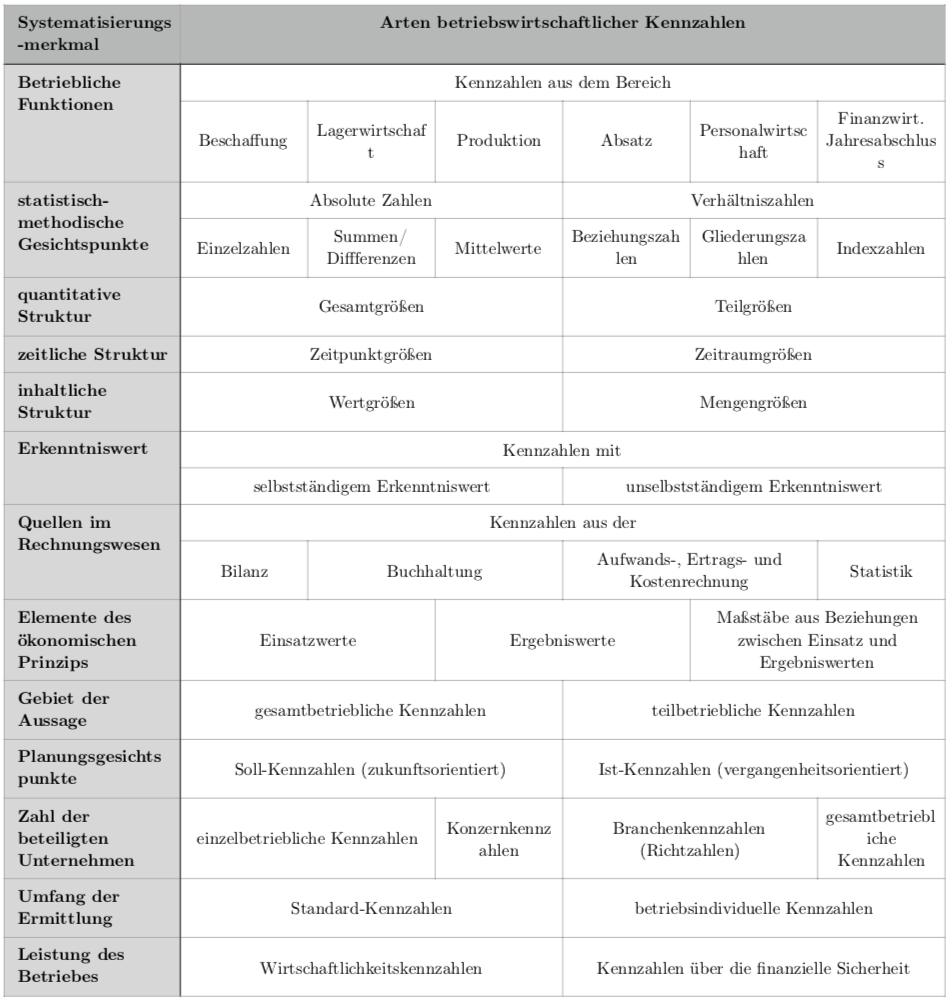
\includegraphics[width=\textwidth]{tab2}
\captionof{table}[Arten betriebswirtschaftlicher Kennzahlen]{Arten betriebswirtschaftlicher Kennzahlen\footnotemark}\label{tab:2}
\end{table}
\addtocounter{footnote}{+0}\footnotetext{Vgl. \cite[S.18]{meyer1989kunden}}
%----Tabelle 
Der Aussagewert einzelner Kennzahlen ist allerdings begrenzt.\footnote{Vgl. \cite[S.41]{Reichmann2017}}
Einzelne Kennzahlen bergen die Gefahr der Fehlinterpretation aufgrund der Tatsache, einen Sachverhalt auf eine einzige Information zu reduzieren.\footnote{Vgl. \cite[S.41]{Reichmann2017}}
Vor diesem Hintergrund ergibt sich die Notwendigkeit einer integrativen Erfassung von Kennzahlen in Kennzahlensystemen, die Abh�ngigkeitsbeziehungen zwischen den Kennzahlen ber�cksichtigen.\footnote{Vgl. \cite[S.41]{Reichmann2017}}
Die Beziehungen zwischen Kennzahlen k�nnen dabei logisch (z.B. definitorisch), empirisch (Ermittlung von Zusammenh�ngen durch Beobachtung) und hierarchisch (z.B. Jahresgewinn der sich aus Monatsgewinnen zusammensetzt) sein.\footnote{Vgl. \cite[S.473]{kuepper2013controlling} und \cite[S.288]{Horvath2015}}
Unter Kennzahlensystemen versteht man im Allgemeinen eine Auswahl von Kennzahlen die die beschriebenen Zusammenh�nge aufweisen und auf ein gemeinsames �bergeordnetes Ziel ausgerichtet sind.\footnote{Vgl. \cite[S.50]{Reichmann2017}, \cite[S.289]{Horvath2015}, sowie \cite[S.96]{weber2015einfuehrung} nach \cite[S.14]{Sandt2004}}
Bei der Zusammenstellung dieser Kennzahlensysteme gibt zwar unterschiedliche Definitionsans�tze, aber eine grundlegende Unterscheidung liegt immer in der ,,Erscheinungsform'':\footnote{Vgl. \cite[S.23]{zentralverband1989zvei}}
\begin{itemize}
	\item Ordnungssystem\\
	Ordnungssysteme stellen Kennzahlen basierend auf ihren sachlichen Zusammenh�ngen zusammen, um bestimmte Aspekte eines Unternehmens zu erfassen.\footnote{Vgl. \cite[S.288]{Horvath2015}}
	\item Rechensystem\\
	Rechensysteme stellen Kennzahlen in rechnerischem Zusammenhang hierarchisch dar.\footnote{Vgl. \cite[S.288]{Horvath2015}} Dadurch ergibt sich in der Regel die Struktur einer Pyramide.\footnote{Vgl. \cite[S.289]{Horvath2015}}
\end{itemize}
Popul�rer Vertreter der Ordnungssysteme ist z.B. die Balanced-Scorecard.\footnote{Vgl. \cite[S.9]{kaplan1996balanced}}
Das bekannteste Rechensystem ist der \gls{ROI}-Baum der E. I. du Pont de Nemours and Company.\footnote{Vgl. \cite[S.7]{davis1950}}\\\\
Das Ziel dieser Arbeit, Flexibilit�t zu bewerten, stellt einen lehrbuchartigen Anwendungsfall eines Kennzahlensystems dar.
F�r die Konzeption ist nun die Auswahl eines Kennzahlensystemkonzepts notwendig.
Bis zu diesem Punkt ist allerdings nicht klar, ob es m�glich ist, Kennzahlen vollst�ndig in rechnerischen und hierarchischen Zusammenhang zu stellen und letztlich eine zentrale Kennzahl zu definieren, die die Spitze einer Pyramidenstruktur darstellen und auch dieser Bedeutung Gen�ge tun kann.
Vielmehr scheint es sinnvoller, Flexibilit�t in verschiedenen Perspektiven zu beleuchten und dadurch auch verschiedene Perspektiven analysier- oder sogar steuerbar zu machen.\footnote{Die Unterscheidung zwischen Analysekennzahlsystemen und Steuerungskennzahlsystemen ist eine weitere M�glichkeit, Kennzahlensysteme einzuordnen, vgl. \cite[S.224-230]{lachnit1976}. Horv\'ath scheint diese gleicherma�en grundlegend wie die oben vorgetragene Unterscheidungsweise einzuordnen, vgl. \cite[S.289]{Horvath2015}. Jedes dieser Systeme m�sste sich jedoch unabh�ngig von dieser Bezeichnung in eine der Kategorien genannten Funktionsweisen einordnen lassen.}
Die Wahl einer Balanced-Scorecard inkl. Definition ihrer Perspektiven scheint daher der geeignetere Ansatz.
\subsubsection{Verrechnungspreise}
Die Ausgangspunkt der Verrechnungspreisproblematik liegt wie angesprochen in der Bildung divisionaler Strukturen.\footnote{Vgl. \cite[S.300]{Horvath2015}}
Die Relevanz des Themas wird an der Tatsache deutlich, dass mehr als die H�lfte des Welthandels, bis zu 70\%, innerhalb von Konzernen abgewickelt wird.\footnote{Die ermittelten Werte variieren von etwas vagen �ber mehr als die H�lfte bis zu 60\% und 70\%, vgl. \cite[S.1]{lohschmidt2005ziele}, \cite[S.378]{baumhoff2014}, \cite[S.497]{crueger2004}, \cite[S.2901]{wehnert2014} und \cite[S.1]{Sauer2018}}
Diese Verrechnungspreise k�nnen sowohl f�r Dienstleistung als auch Produkte gebildet werden, die innerhalb eines Unternehmens oder Konzerns angeboten und ,,gekauft'' bzw. ,,verkauft'' werden.
Auf diese Weise wird der ,,marktliche Koordinationsmechanismus''\footnote{Vgl. \cite[S.300]{Horvath2015}} zwischen weniger unabh�ngigen Wirtschaftssubjekten zu etablieren.
Einerseits beherbergt dieses Verfahren ,,institutionen�konomische'' Vorteile, andererseits rechtfertigt die durch die Verkn�pfung der Unternehmenseinheiten optimierte Koordination und Steuerung den internen Leistungsbezug.\footnote{Vgl. \cite[S.2-3]{battenfeld1999}}
Die Verrechnungspreise bilden sich dabei nicht nat�rlich im Marktgef�ge, sondern werden von Entscheidungstr�gern festgelegt.\footnote{Vgl. \cite[S.170]{Kilger2012}}
Neben der Steuerung des Leistungsbezugs �ber den Preis\footnote{In diesem Zusammenhang werden Verrechnungspreise h�ufig Lenkpreise genannt, vgl. \cite[S.301]{Horvath2015}} ist �ber die Verrechnung eine divisionsspezifische Erfolgsermittlung m�glich.\footnote{Vgl. \cite[S.302]{Horvath2015}}
Die Marktann�herung der Preise ist so ernstzunehmen, dass Steuerpr�fungen diese mittlerweile ber�cksichtigen.\footnote{Vgl. \cite{Rieke2015} und \cite{Sauer2018}}
\\\\
Unabh�ngig von der Rollenkonzeption\footnote{Vgl. dazu \cite[S.581f]{schroederHMD2016}} einer internen IT-Abteilung sind diese in der Tat interne Leistungserbringer.
Bestimmte Gr��enordnungen erm�glichen sogar die vollst�ndige Ausgr�ndung als Konzerntochter\footnote{Vgl. \cite[S.264]{Gadatsch2014}} mit entsprechender Verrechnung an �brige Konzernorgane.
Insofern ist die Bildung von Verrechnungspreisen f�r IT-Leistungen einschl�gig und umfasst neben direkter Dienstleistungsverrechnung ggf. auch die Bildung von Kostenstellen zur Verrechnung von Abschreibungen oder leistungsbezogen extern beschaffter Leistung und Produkte.\footnote{Vgl. \cite{Gadatsch2013Kostenrechnung}}
Auch die Tatsache, dass die Unternehmens-IT immer st�rker im Wettbewerb mit Services aus der Cloud stehen, die von Fachbereichen mit geringem initialen Aufwand beschafft werden k�nnen, rechtfertigt die Marktorientierung der Leistungsverrechnung.\\
Im Zentrum dieser Ausf�hrungen steht allerdings die Frage, inwieweit der Lenkungsansatz des Controllings in der IT hinsichtlich Flexibilit�t Verrechnungspreisen zu konzipieren ist.
Diesbez�glich scheint Flexibilit�t, sofern nachweisbar als Werttreiber, mehr ein Entscheidungskriterium einer Leistung oder eines Produkts zu sein als in die Verrechnung zu integrierender Faktor.
Die Verechnungsmethoden des IT-Controllings sind bereits insoweit differenziert, als Modelle definiert sind, die z.B. direkte, prozessorientierte oder produktorientierte Verrechnung erm�glichen und daher ausreichend Reaktionsm�glichkeiten bieten.\footnote{Vgl. \cite[S.195-199]{kesten2013}}

\section{Produktionscontrollings}
\subsection{Definition}\label{DefinitionProduktionscontrolling}
Nachdem in \ref{Produktionscontrolling} das \gls{Pr-C} aufgrund seiner zu Flexibilit�t einschl�gigen Inhalte als aussichtsreiches Portfolio identifiziert wurde, ist es erforderlich, das \gls{Pr-C} umfangreich zu erfassen, die Methoden und Techniken zu strukturieren und auf Einschl�gigkeit zu Flexibilit�t zu pr�fen und schlie�lich eine Auswahl von in der Konzeption einzuschlie�enden bzw. zu �bertragenden Elementen zu formulieren. 
Grunds�tzlich ist das \gls{Pr-C} die Disziplin bzw. betriebliche T�tigkeit, die dazu dient, die Anspr�che des Controllings in der Produktion zu platzieren und umzusetzen.\footnote{Vgl. \cite[S.20]{Gottmann2019}}
Die Produktion hat dabei die Aufgabe, Wertsteigerung von Produkten zu erwirken, indem ein Input einem Output gegen�bergestellt wird.\footnote{Vgl. \cite[S.20]{Gottmann2019}}
Dabei handelt es sich neben direktem Input in Form von Produktionsanlagen, Material und Arbeitsleistung auch um indirekten Input wie die Organisation, Planung und Steuerung.\footnote{Vgl. \cite[S.19]{Gottmann2019}}
Das Controlling, dessen Ziel wiederum die ergebnisorientierte Planung und Steuerung von Ma�nahmen durch Beschaffung, Aufbereitung, Analyse und Kommunikation von Daten ist\footnote{Vgl. \cite[S.20]{Gottmann2019}}, muss also in den entscheidenden Parametern auf die Produktion und die kaufm�nnischen Zielsetzungen ausgerichtet werden\footnote{Vgl. \cite[S.20]{Gottmann2019}} und letztlich einen effizienten und erfolgreichen Betrieb sicherstellen\footnote{Vgl. \cite[S.20]{Gottmann2019}}, eine ganzheitliche Optimierung von Investitionsentscheidungen zu erm�glichen\footnote{Vgl. \cite[S.20]{Gottmann2019}} und vor allem Kompromisse zwischen bei den kaufm�nnischen und produktionsrelevanten Zielsetzungen\footnote{Vgl. \cite[S.20]{Gottmann2019}, \cite{schnell2018produktion} und \cite[S.24-26]{klein2012controlling1} sowie} zu finden. 
Dahingehend ist es also Aufgabe des \gls{Pr-C}, Produktions- und Controllingziele zu verbinden\footnote{Vgl. \cite[S.21]{Gottmann2019}} , den angesprochenen Input und Output zu optimieren\footnote{Vgl. \cite[S.21]{Gottmann2019}} und daf�r die richtigen Instrumente ausw�hlen, zu implementieren und einzusetzen.\\
Das \gls{Pr-C} differenziert in seinen T�tigkeiten die zeitlichen Dimensionen grunds�tzlich.
Je nach Interpretation wird lediglich zwischen strategischem und taktisch-operativen \gls{Pr-C} unterschieden\footnote{Vgl. \cite[S.25]{klein2012controlling1}}, w�hrend andere auch letzteres als unterschiedliche Dimensionen auslegen.\footnote{Vgl. \cite[S.9]{Gottmann2019}}
Letztlich ist die Controlling-Konzeption dabei aufgrund der Mangementunterst�tzung immer am Management-System auszurichten.
Auch hierbei ist eine Unterscheidung nach strategischem\footnote{Vgl. \cite[S.20]{zaepfel2014strategisches}}, taktischem\footnote{Vgl. \cite[S.20]{zaepfel2010taktisches}} und operativem\footnote{Vgl. \cite[S.20]{zaepfel1982operatives}} Produktionsmanagement m�glich.
Eine m�gliche Auslegung ist z.B., in der strategischen Perspektive langfristige Ziele innerhalb des Marktes zu betrachten, in der taktischen das Produktionsprogramm in Breite und Tiefe zu fokussieren und in der operativen die laufenden Fertigungsauftr�ge.\footnote{Vgl. \cite[S.4]{zaepfel2010taktisches}} 
\\\\
Die Begriffe des \gls{P-C}, der Produktionsplanung und des Produktionsmanagement sind nicht vollst�ndig klar gegeneinander abzugrenzen.
Gottmanns Definition schlie�t Planung als Bestand des \gls{P-C} ein, w�hrend z.B. L�dding die Planung als prim�ren Vorgang beschreibt und das \gls{P-C} davon trennt und im Controlling-Aspekt lediglich die operative Zielerreichungsbestimmung sieht.\footnote{Vgl. \cite[S.120-121]{Loedding2016}} 
Zwar w�re das Produktionsmanagement als F�hrungsaufgabe der Produktion, die durch das \gls{P-C} zu unterst�tzen ist, logisch von diesen abzugrenzen, doch es existieren Definitionsans�tze zum Produktionsmanagement, die darin ebenfalls Planung und Steuerung verorten und dazu deutlich �berschneidende Methodenportfolios vorschlagen.\footnote{Vgl. \cite[S.6]{grap1998produktion}}\\
Hier stellt sich nun die Frage, inwieweit die Differenzierung der Funktionsbereiche dem Vorhaben dieser Arbeit zutr�glich ist.
Da vor allem der Gesamtbereich der planerischen und steuernden Aspekte der Produktion einschl�gige �berlegungen zu Flexibilit�t aufweist und deren �bertragbarkeit gepr�ft werden soll, scheint eine harte Begriffstrennung insofern nicht hilfreich, als dass Methoden aufgabenbereichs�bergreifend zum Einsatz kommen k�nnen.
Die Unterscheidung  der zeitlichen Planungshorizonte (strategisch, taktisch, operativ) ist ferner �bergreifend in immer �hnlicher Auslegung zu bemerken, sodass eine weniger strikte Trennung dar�ber hinaus nicht trivialisierend scheint.
Die alleinige Betrachtung von Steuerungsmethoden, also die Ausklammerung von Planungsmethoden w�re sowieso eine unangemessene Reduktion des Untersuchungsbereichs.
\subsection{Betrachtungsgegenst�nde}
\subsubsection{Bedarfsplanung}
%bild produktionsplanung
\todo{einleiten mit produktionsplanungsprozess}
\begin{itemize}
\item Prim�rbedarf\\
Die Prim�rbedarfsplanung ermittelt die herzustellende Menge der zum Absatz bestimmten, d.h. verkaufsf�higen Erzeugnisse, Baugruppen oder Einzelteile nach Art, Menge und Termin bzw. Planungsperiode.\footnote{Vgl. \cite[S.199]{Abts2017} und \cite[S.108]{Loedding2016}}
Dieser Prozess wird ma�geblich durch Kalkulation bestehender Auftr�ge sowie Absatzprognosen auf der einen Seite und maschinelle sowie personelle Kapazit�t auf der anderen Seite beeinflusst.\footnote{Vgl. \cite[S.199]{Abts2017}}
Ebenfalls gel�ufig ist die Bezeichnung Produktionsprogramm bzw. Produktionsprogrammplanung.\footnote{Vgl. \cite[S.108]{Loedding2016}}
\item Sekund�rbedarf\\
Der darauf aufbauende Materialbedarf bzw. Sekund�rbedarf und dessen Planung ermittelt anhand von St�cklisten oder fr�herer Verbrauchswerte abz�glich Lagerkapazit�ten\footnote{Vgl. \cite[S.200]{Abts2017}} den f�r den Prim�rbedarf notwendige Menge an Komponenten und Teilen und ordnet diese periodengerecht zu\footnote{Vgl. \cite[S.110]{Loedding2016}}.
\item Terti�rbedarf\\
Dar�ber hinaus kann ein Terti�rbedarf erfasst werden, der den Bedarf an Betriebs- und Hilfsstoffen sowie Verschlei�material\footnote{Vgl. \cite[S.104]{Pfohl2018}} anzeigt.\footnote{Vgl. \cite[S.243]{Alpar2019}}
\end{itemize}
Die ermittelten Sekund�r- und Terti�rbedarfe stellen zun�chst grunds�tzlich Bruttobedarfe dar, die sich durch Lagerbestandsfortschreibung in Nettobedarfe �berf�hren lassen.\footnote{Vgl. \cite[S.243]{Alpar2019}}\\
Die Zusammenh�nge sind in Abbildung \ref{img:Materialbedarfsarten} dargestellt.
%Bild ->
\begin{figure}[!htb]
\centering
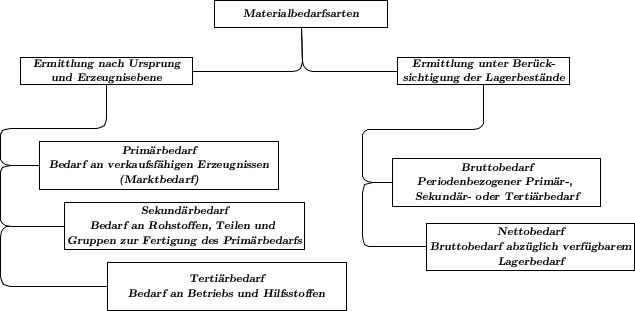
\includegraphics[width=1\linewidth]{pfohl_Materialbedarfsarten}
\captionof{figure}[Materialbedarfsarten]{Materialbedarfsarten\footnotemark}
\label{img:Materialbedarfsarten}
\end{figure}
%Bild <-
\addtocounter{footnote}{+0}\footnotetext{\cite[S.287]{hartmann2002materialwirtschaft}}
Die Berechnungsmethoden f�r die skizzierten Zwecke werden literatur�bergreifend unterschieden zwischen deterministischen, stochastischen und Sch�tzungs-Ans�tzen.\footnote{Vgl. \cite[S.284]{hartmann2002materialwirtschaft}, \cite[S.105]{Pfohl2018} und \cite[S.443ff und S.489ff]{Schoensleben2016}}
\begin{itemize}
\item Deterministisch Verfahren\\
Deterministische Verfahren existieren sowohl analytischer als auch synthetischer Natur.
W�hrend analytische Verfahren die exakte Kalkulation anhand von St�cklisten vornehmen\footnote{Vgl. \cite[S.105]{Pfohl2018}}, geht die synthetische Bedarfsermittlung mit Teileverwendungsnachweisen an die Ermittlung heran.\footnote{Vgl. \cite[S.105]{Pfohl2018}}
Deterministische Verfahren sind deduktiv.
\item Stochastisch Verfahren\\
Stochastische nutzen zur Bedarfsermittlung historische Verbrauchsdaten vergleichbarer Produktionen.
Auf deren Basis wird eine Prognose der geplanten Produktion vorgenommen.\footnote{Vgl. \cite[S.106]{Pfohl2018}}
Je nach Tendenz (steigend, gleichbleibend) sind daf�r Methoden wie die Mittelwerbildung, exponentielle Gl�ttung oder Regressionsrechnung m�glich.\footnote{Vgl. \cite[S.106]{Pfohl2018}}
Stochastische Verfahren sind induktiv.
\item Sch�tzverfahren\\
Sind f�r keine der beiden genannten Methoden die Voraussetzungen gegeben, so bleiben lediglich Sch�tzmethoden �brig.
Hierbei ist lediglich zu unterscheiden zwischen rein intuitiven Sch�tzungen einer oder mehrerer Personen und logisch begr�ndbaren und damit intersubjektiv �berpr�fbaren Sch�tzungen.\footnote{Vgl. \cite[S.106]{Pfohl2018}}
\end{itemize}
Die Zusammenh�nge der Berechnungsmethoden sind in Abbildung \ref{img:berechnungsmethoden} dargestellt.
%Bild ->
\begin{figure}[!htb]
\centering
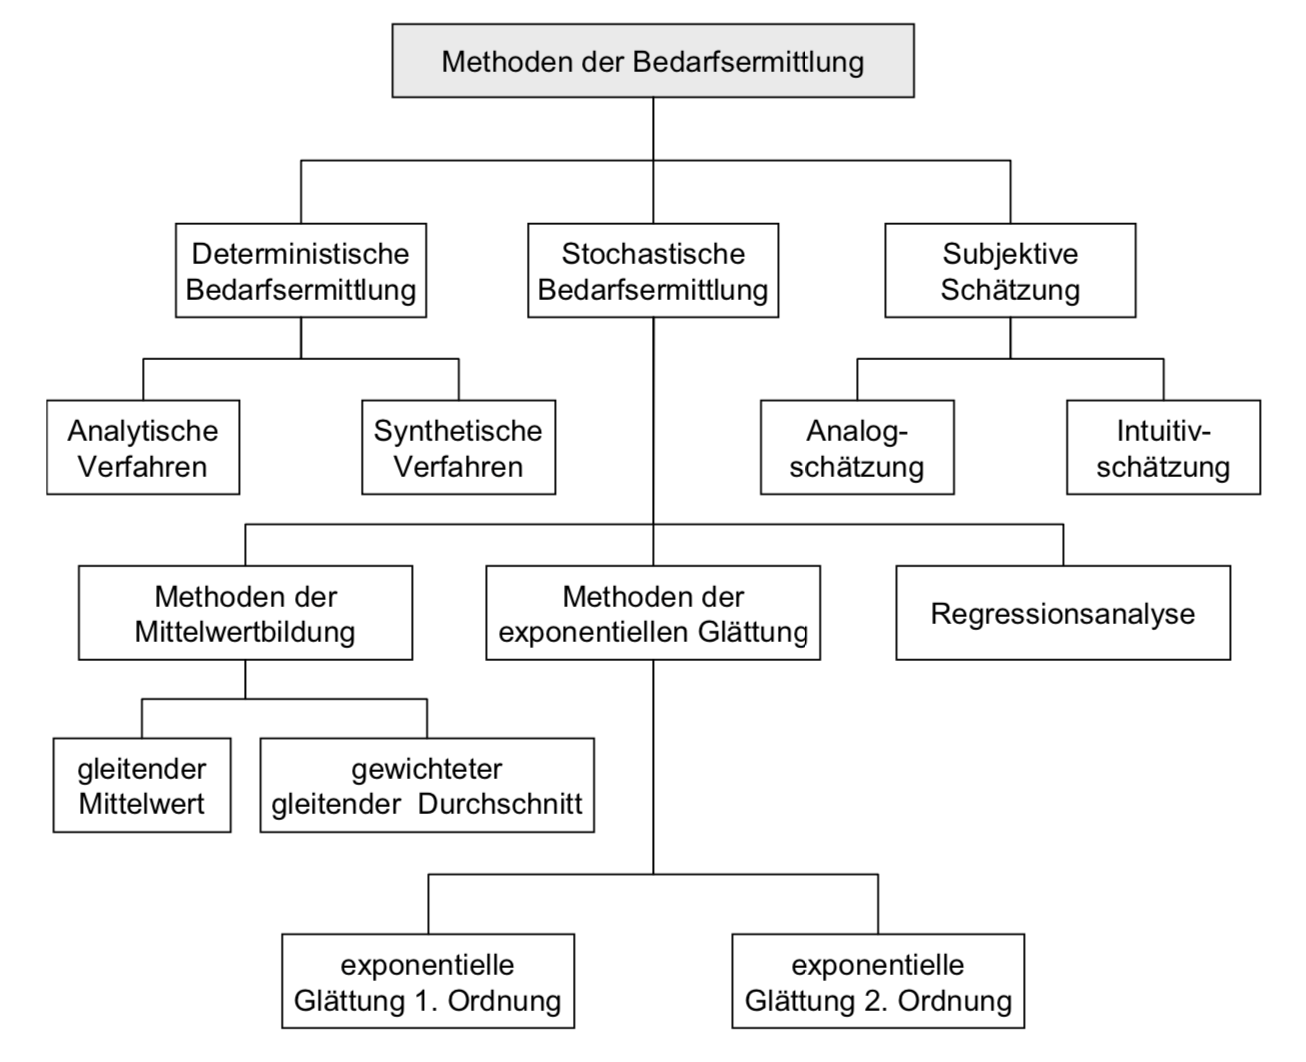
\includegraphics[width=1\linewidth]{methoden_bedarfsermittlung}
\captionof{figure}[Methoden der Bedarfsermittlung]{Methoden der Bedarfsermittlung\footnotemark}
\label{img:berechnungsmethoden}
\end{figure}
\addtocounter{footnote}{+0}\footnotetext{\cite[S.289]{hartmann2002materialwirtschaft}}
%Bild <-
%---------------
%LOSGR�SSEN
\subsubsection{Losgr��en}
	Ein Los besteht ,,aus einer bestimmten Anzahl konstruktiv und technologisch gleicher oder �hnlicher Einzelteile, die unabh�ngig davon, ob sie zu einem oder mehreren Endprodukten geh�ren, gemeinsam in einem Fertigungsauftrag unter einmaliger Gew�hrung der R�stzeit\footnote{,,Als R�sten bezeichnet man den Vorgang, die Maschine auf die Fertigung eines neuen Teiles oder Loses einzurichten. Teil des R�stens sind auch Probel�ufe der Maschine.'' - \cite[S.182]{vahrenkamp2008produktionsmanagement}} je Arbeitsgang und Arbeitsplatz gefertigt werden.''\footnote{\cite[S.670]{nebl2007produktionswirtschaft}}
	Eine Losgr��e beschreibt demnach die Menge gleichartiger Objekte, die nacheinander in einem R�stvorgang angefertigt werden.
	Losgr��en sind sowohl f�r Prim�r- als auch Sekund�r- und Terti�rbedarf festzulegen.\footnote{Vgl. \cite{siepermann2018}}
	Bei der Losgr��enplanung handelt sich um ein Methodenportfolio zur Kosten- oder Flussoptimierung\footnote{Vgl. \cite[S.153]{vahrenkamp2008produktionsmanagement}}
	Es wird zwischen Durchlaufzeitminimierung, Flussoptimierung mit Engpassber�cksichtigung, Kostenminimierung und Lager- und-Produktionskostenoptimierung unterschieden.
	\begin{itemize}
		\item Durchlaufzeitminimierung\\
		Der Ansatz durchlaufzeitminimaler Lose stammt aus der Lean Production\footnote{Vgl. \cite[S.154]{vahrenkamp2008produktionsmanagement}} und fokussiert exklusiv die Minimierung der Produktionszeit eines Loses.\footnote{Vgl. \cite[S.154]{vahrenkamp2008produktionsmanagement}}
		Die R�stvorg�nge werden dabei genau wie die Produktionsvorg�nge lediglich hinsichtlich der Dauer betrachtet.\footnote{Vgl. \cite[S.154]{vahrenkamp2008produktionsmanagement}}
		Das Verfahren versucht zu hohen Anteil an R�stzeiten gegen�ber zu langer Bearbeitungsdauer zu optimieren.\footnote{Vgl. \cite[S.154]{vahrenkamp2008produktionsmanagement}}
		\item Flussoptimierung mit Engpassber�cksichtigung\\
		Wie auch die Durchlaufzeitminimierung besteht auch dieser Ansatz in zeitlicher Optimierung.\footnote{Vgl. \cite[S.155]{vahrenkamp2008produktionsmanagement}}
		Der Ansatz ist vor allem dann relevant, wenn verschiedene Produkte in vorgegebenem Zyklus hintereinander auf einer Maschine produziert werden muss.
		Die Problematik besteht weniger in diesem Vorgang als in der Synchronisierung mit anschlie�enden Vorg�ngen die von dessen Erzeugnissen abh�ngig sind bzw. darauf aufbauen.\footnote{Vgl. \cite[S.155]{vahrenkamp2008produktionsmanagement}}
		Das Verfahren stimmt die Losgr��e auf den Bedarf ab.\footnote{Vgl. \cite[S.155-157]{vahrenkamp2008produktionsmanagement}}
		\item Kostenminimierung\\
		Die Kostenminimierung ist hingegen ein klassisches betriebswirtschaftliches Losgr��enbestimmungsverfahren.
		Die fixen R�stkosten zuz�glich der variablen Herstellungskosten sind rein �konomisch anhand des Bedarfes und der m�glichen Laufzeiten so zu kalkulieren, dass die Kosten m�glichst gering sind.\footnote{Vgl. \cite[S.158]{vahrenkamp2008produktionsmanagement}}
		\item Lager- und-Produktionskostenoptimierung\\
		In diesem Verfahren werden zus�tzlich zu R�st- und Produktionskosten die Lagerkosten ber�cksichtigt und das Verh�ltnisse f�r einen isolierten Teil der Produktionsstufe optimiert.\footnote{Vgl. \cite[S.159]{vahrenkamp2008produktionsmanagement}}
		Die Pr�misse des Verfahrens ist, dass Erzeugnisse mit Fertigstellung Lagerkosten verursachen.
		Dabei sind vor allem h�ufige R�stkosten hohen Lagerkosten gegen�ber zu optimieren.
		Die optimale Losgr��e nach Andler z.B. ermittelt eine Losgr��e, welche die Summe von R�st- und Lagerkosten minimiert und ist auch auf Einkaufslosgr��en �bertragbar, wenn R�stkosten durch bestellfixe Kosten ersetzt werden.\footnote{Vgl. \cite{andler1929}}
	\end{itemize}
	Die Berechnungsmethoden f�r die skizzierten Zwecke sind entweder statischer oder dynamischer Natur.\footnote{Vgl. \cite[S.284]{hartmann2002materialwirtschaft}, \cite[S.105]{Pfohl2018} und \cite[S.443ff und S.489ff]{Schoensleben2016}}
	\begin{itemize}
		\item Statische Verfahren
		Statische Verfahren wie der Ansatz von Andler verwenden lediglich die Kosten (R�st-, Lager- und variable Produktionskosten) und berechnen die Losgr��e einer Planungsperiode.\footnote{Vgl. \cite[S.162]{vahrenkamp2008produktionsmanagement}}
		\item Dynamische Verfahren
		Dynamische Verfahren sind dagegen auf zeitlich ver�nderliche Nachfragemengen ausgerichtet.
		Au�erdem existieren Verfahren f�r ein- und mehrstufige Verfahren.
	\end{itemize}	
	%---------------
%TERMIN- und KAPAZIT�TSPLANUNG	
\subsubsection{Termin- und Kapazit�tsplanung}
\todo{In der Leseprobe von Vahrenkamp fehlten hier Seiten}
Nach Abschluss der Planung der Produktionsmengen ist festzulegen, in welcher Weise Auftr�ge die Produktion zu durchlaufen\footnote{Vgl. \cite[S.181]{vahrenkamp2008produktionsmanagement}} haben und welche Zeitstrukturen dabei einzuhalten sind.\footnote{Vgl. \cite[S.214]{Abts2017}}
Dabei ist auch die Kapazit�t von Infrastruktur und Personal zu ber�cksichtigen.\footnote{Vgl. \cite[S.200]{Abts2017} und \cite[S.181]{vahrenkamp2008produktionsmanagement}}
Der Planungsprozess setzt sich aus der Durchlauf- und Kapazit�tsterminierung zusammen.\footnote{Vgl. \cite[S.181]{vahrenkamp2008produktionsmanagement}}\\
%Durchlaufterminierung
Die Durchlaufterminierung legt vorl�ufige Star- und Endtermine der Arbeitsvorg�nge sowie deren Koordination grob fest.\footnote{Vgl. \cite[S.181]{vahrenkamp2008produktionsmanagement}}
Kapazit�tsrestriktionen bleiben bis zu diesem Punkt unber�cksichtigt.\footnote{Vgl. \cite[S.181]{vahrenkamp2008produktionsmanagement}}
Zentraler Aspekt bei dieser Planung ist die Arbeitsplatzdurchlaufzeit, die die Zeitspanne f�r jeden Arbeitsschritt definiert, um diesen zwischen dem davor und dem danach liegenden Arbeitsschritt einzuordnen.\footnote{Vgl. \cite[S.182]{vahrenkamp2008produktionsmanagement}}
Die Arbeitsplatzdurchlaufzeit setzt sich dabei aus aus den Komponenten Transportzeit, Wartezeit, R�stzeit und der eigentlichen Bearbeitungszeit zusammen\footnote{Vgl. \cite[S.182]{vahrenkamp2008produktionsmanagement}}, vgl. Abbildung \ref{img:arbeitsplatzdurchlaufzeit}, wobei sowohl ablauforganisatorische oder technische Gr�nde f�r Wartezeit verantwortlich sein k�nnen (z.B. Materialaush�rtung).\footnote{Vgl. \cite[S.181]{vahrenkamp2008produktionsmanagement}}
%Bild ->
\begin{figure}[!htb]
\centering
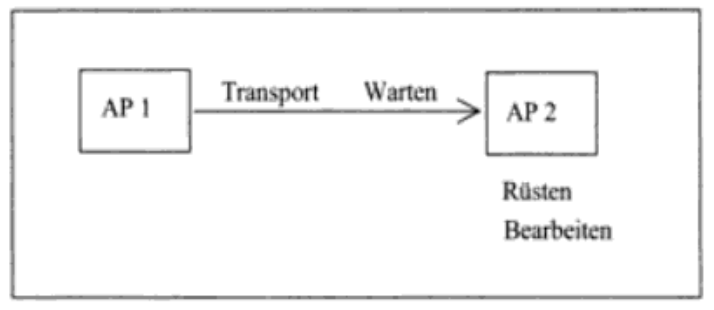
\includegraphics[width=0.5\linewidth]{arbeitsplatzdurchlaufzeit}
\captionof{figure}[Arbeitsplatzdurchlaufzeit]{Arbeitsplatzdurchlaufzeit\footnotemark}
\label{img:arbeitsplatzdurchlaufzeit}
\end{figure}
\addtocounter{footnote}{+0}\footnotetext{\cite[S.182]{vahrenkamp2008produktionsmanagement}}
%Bild <-
Die Summe aller Arbeitsplatzdurchlaufzeiten ergibt die Sch�tzung f�r die Durchlaufzeit eines gesamten Auftrags.
Aufgrund m�glicher Konkurrenzen um Arbeitsstationen k�nnen sich Wartezeiten ver�ndern und, da R�stzeiten reihenfolgen- und zustandsabh�ngig sind, k�nnen sich diese ebenfalls ver�ndern, sodass ohne Kapazit�tsber�cksichtigung die Durchlaufzeitenkalkulatio lediglich eine zu interpretierende Sch�tzung darstellt.\footnote{Vgl. \cite[S.182]{vahrenkamp2008produktionsmanagement}}
Der Pfad der Gesamtdurchlaufzeit stellt den kritischen Pfad der Produktion dar.\footnote{Begriff aus der Netzplantechnik, vgl. \cite[S.182]{vahrenkamp2008produktionsmanagement}}
Mithilfe von Vorw�rts- oder R�ckw�rtsterminierung werden letztlich alle Zeitpunkte bzw. Termine f�r die Produktion festgelegt.\footnote{Vgl. \cite[S.184-185]{vahrenkamp2008produktionsmanagement}}\\\\
%Kapazit�tsterminierung
Aus der Durchlaufterminierung resultieren terminierte Auftr�ge, deren Durchf�hrbarkeit noch nicht best�tigt ist.\footnote{Vgl. \cite[S.185]{vahrenkamp2008produktionsmanagement}}
Diese Verifikation ist Aufgabe der Kapazit�tsterminierung in Form der Ermittlung von Unter- bzw. �berauslastungen, die untereinander ausgeglichen werden m�ssen.\footnote{Vgl. \cite[S.200]{Abts2017}}
M�gliche Kapazit�tseinschr�nkungen resultieren aus Wartungs- und Instandhaltungsarbeiten, Produktionsst�rungen sowie Urlaubs- und Krankheitszeiten des Personals.\footnote{Vgl. \cite[S.200]{Abts2017}}
Solche Kapazit�tsengunstimmigkeiten bedingen entweder die Anpassung des Kapazit�tsangebots an die Kapazit�tsnachfrage (Kapazit�tsanpassung) oder umgekehrt (Belastungsanpassung).\footnote{Vgl. \cite[S.126-128]{kurbel2016enterprise},\\ \cite[S.186-187]{vahrenkamp2008produktionsmanagement},\\ \cite[S.190-193]{zaepfel2010grundzuege} und\\ \cite[S.689-690]{schweitzer1994industriebetriebslehre}}
Kapazit�tsanpassungen sind z.B. m�glich durch zeitliche Modifikation (�berstunden oder Kurzarbeit bei �berlastung, Schichtabbau bei Unterlastung, etc.), Intensit�tsanpassung (Durchsatzerh�hung oder -verringerung durch Anpassung der Produktionsgeschwindigkeit) oder quantitativer Anpassung (Nutzung von Reserven bei �berlastung, tempor�re Stilllegung bei Unterlastung, Umschichtung von Personal aus anderen Bereichen, etc.).\footnote{Vgl. \cite[S.267-269]{kiener2012produktions} \cite[S.229]{guenther2011produktion}}\\\\
Belastungsanpassungen sind z.B. durch zeitliche Verschiebung von Fertigungsauftr�gen, die nicht bereits zum fr�hesten Zeitpunkt geplant sind, auf Zeitpunkte mit geringerer Auslastung zu realisieren.
Ferner sind Stauchungen und Streckungen durch geringere oder h�here Kapazit�tsinanspruchnahme m�glich, Anpassung der Auftragsgr��e (falls nur ein Teil des Loses zur Auftragserf�llung notwendig ist (�berlastung) oder �berproduzierte Errzeugnisse auf Lager gelegt werden k�nnen (Unterlastung)), externe Auftragsvergabe bis hin zu Auftragsverzicht (�berlastung) oder Auftragsannahme (Unterlastung) oder, sofern technisch m�glich, alternative Durchf�hrung von Arbeiten auf anderen Betriebsmitteln.\footnote{Vgl. \cite[S.269-271]{kiener2012produktions} und\\ \cite[S.716-720]{Nebl2011}}\\
Die Ma�nahmen sind dabei nicht immer klar voneinander abzugrenzen, da z.B. Intensit�tsanpassungen auch Stauchungen bzw. Streckungen bedingen.
\subsubsection{Auftragsfreigabe}
\subsubsection{Ablaufplanung}



\subsection{Teilbereiche}
%https://refa.de/service/refa-lexikon/produktionsmanagement mal gucken
\subsubsection{Strategisches Produktionscontrolling}
\subsubsection{Taktisches Produktionscontrolling}
\subsubsection{Operatives Produktionscontrolling}
\subsection{Methoden und Techniken}
KLR selbst digital extrem relevant\cite{kuenzel2018}

\subsubsection{Strategische Instrumente}
\paragraph{Produktlebenszyklus-Analyse}
\paragraph{Balanced Scorecard}
\subsubsection{Operative Instrumente}
\paragraph{Kennzahlen}
\paragraph{Kennzahlensysteme}
%\section{Grundlagen des IT-Controllings}
\subsection{Definition}
\subsection{Einbettung in das IT-Management}
\subsection{Organisation }
\subsection{Ziele und Aufgaben}
\subsection{Teilbereiche}
\subsubsection{IT-Portfoliocontrolling}
\subsubsection{IT-Projektcontrolling}
\subsubsection{IT-Produktcontrolling}
\subsubsection{IT-Infrastrukturcontrolling}
\subsection{Methoden und Techniken}
\subsubsection{IT-Kennzahlen}
\subsubsection{IT-Balanced Scorecard}
\subsubsection{IT-Kosten- und Leistungsrechnung}
\subsubsection{Total Cost of Ownership}
\subsubsection{IT-Outsourcing}
\section{Flexibilit\"at}
\subsection{Allgemeines Verst\"andnis von Flexibilit\"at}
\subsection{Flexibilit\"at im Anwendungskontext}
\subsubsection{Flexibilit\"at im Kontext der Produktion}
\subsubsection{Flexibilit\"at im Kontext der IT-Organisation}
\subsubsection{Messung und Bewertung von Flexibilit\"at}
\paragraph{Bewertungsans\"atze im Produktionscontrolling}
\todo{"Steuerungsinstrument" aus Kapitel 2 aufgreifen, auf Arten der Steuerungsinstrumente eingehen}
\subparagraph{Strategische Flexibilit\"at}
\subparagraph{Taktische Flexibilit\"at}
\subparagraph{Operative Flexibilit\"at}
\paragraph{\"Ubertragbarkeit auf das IT-Controlling}
\subparagraph{Flexibilit\"at im IT-Portfoliocontrolling}
\subparagraph{Flexibilit\"at im IT-Projektcontrolling}
\subparagraph{Flexibilit\"at im IT-Produktcontrolling}
\subparagraph{Flexibilit\"at im IT-Infrastrukturcontrolling}
\section{Rahmenwerk zur Bewertung}
\subsection{Konzeptionelle Idee}
Da wie dargelegt Wechselwirkungen zwischen verschiedenen flexibilisierbaren Betrachtungsgegenst�nden in der IT bestehen, scheint es naheliegend, diesen Ansatz zur Integration in einem Rahmenwerk zur Bewertung der IT-Flexibilit�t zu nutzen.
Einerseits existieren wie dargelegt M�glichkeiten zum gezielten Aufbau von Flexibilit�tspotentialen in verschiedenen Dimensionen bzw. f�r verschiedene Betrachtungsgegenst�nde, deren Implementation wie angegeben beurteilbar ist, andererseits sind dadurch Effekte zu erzielen, deren Auftreten ebenfalls messbar ist.\\
Insofern besteht also ein integriert operationalisierbares Konstrukt, das zur koh�renten Steuerung des Aufbaus dieser Flexibilit�tspotentiale und gleichzeitig dauerhaft zur �berpr�fung des Nutzens genutzt werden kann.
Die Ma�nahmen zum Aufbau der Flexibilit�tspotentiale entsprechen kurz-, mittel- und langfristigen Vorhaben, da z.B. Infrastrukturaufbau aufgrund des 72-monatigen Abschreibungszeitraums eher als strategische Investition get�tigt wird\footnote{Vgl. \cite[6.14.3.1]{afa-tabelle}}, Personalentwicklung ebenfalls eine langwierige Aufgabe ist, aber die Durchf�hrung von agilen Softwareprojekten zur Herstellung von Microservices durchaus auch k�rzere Zeitr�ume als ein Jahr in Anspruch nehmen kann. 
Unter Ber�cksichtigung der Tatsachen, dass die Ma�nahmen sowohl strategischer als auch taktisch-operativer Natur sein k�nnen ist das Konzept der \gls{BSC} die angemessenste Variante zur Modellierung der bisherigen Konzeption.
\subsection{Dimensionsdefinition}
Wie in \ref{BSC} angesprochen ist die Voraussetzung f�r die Koh�sion der mit einer \gls{BSC} angestrebten Steuerung in der Definition von Ursache-Wirkungs-Ketten der Dimensionen.
Je nach Vorhaben ist allerdings vorher sogar eine Definition der zu untersuchenden Dimensionen vorzunehmen.\\
Unter Ber�cksichtigung der in \ref{adaptionbetrachtungsgegenstaende} ermittelten Betrachtungsgegenst�nde sind diesbz�gliche Kandidaten ersichtlich, sodass als Dimensionen der Flexibilit�t Personal, die technologischen Sichtweisen Infrastruktur/Software sowie die Projekte in Frage kommen.
Zur ganzheitlichen Steuerung eines Unternehmens sind zudem der Einfluss auf die Kunden- sowie die Finanzperspektive zu ber�cksichtigen.
Als Basis von Gesch�ftsprozessen ist die Interpretation der IT-Dienste als Substitution der Prozessperspektive eine im Modellierungsvorhaben sinnvolle Abwandlung einzustufen.
Die Aggregation der flexibilit�tstragenden Betrachtungsgegenst�nde in einer Dimension, die die Lern- und Entwicklungsperspektive ersetzt, ist eine Ma�nahme, die bereits in �hnlicher Weise Vorhaben f�r produktionswirtschaftliche Flexibilit�t gepr�gt hat.\footnote{Vgl. \cite[S.9]{winkler2008} und \cite[S.57]{Kempkes2018}.}
Mit dieser Konstellation k�nnen nun Wirkungsketten modelliert werden.
Dieses Vorhaben sollte in der Praxis Top-Down mit der Direktive finanziellen unternehmerischen Erfolgs als Ausgangspunkt erfolgen\footnote{Vgl. \cite[S.9]{horvath1998balanced}}.\\
Ausgehend von der Lern- und Entwicklungsperspektive, die durch die Flexibilit�tspotentiale ersetzt wird, kann alternativ auch eine Bottom-Up-Modellierung vorgenommen werden.\footnote{Vgl. \cite[S.181ff]{horvath2001} nach \cite[S.141]{siebert2011balanced}.}
 \begin{figure}[!htb]
\centering
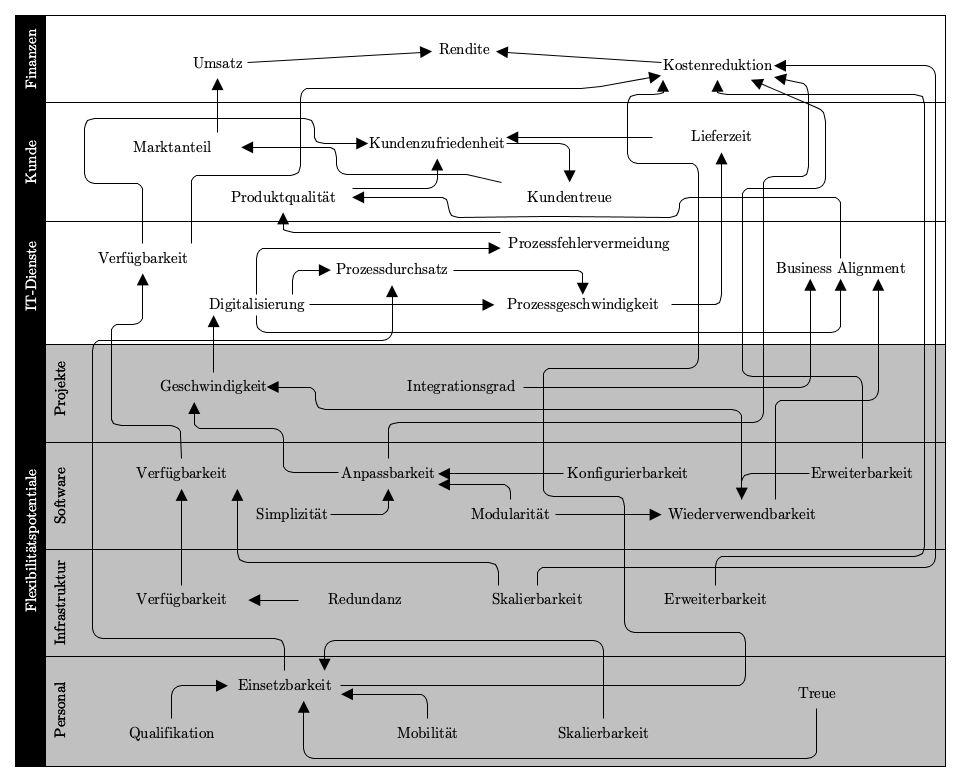
\includegraphics[width=0.8\linewidth]{bsc_wirkungsketten}
\captionof{figure}[FlexIT]{Wirkungsketten\footnotemark}
\label{img:wirkungsketten}
\end{figure}
\addtocounter{footnote}{+0}\footnotetext{Eigene Darstellung in Anlehnung an}
Die ausgew�hlten Ziele der Kunden- und Finanzperspektive sind �bliche Aspekte der Unternehmenssteuerung\footnote{Vgl. zur Auswahl \cite[S.181ff]{horvath2001} nach \cite[S.141]{siebert2011balanced} sowie zur Modellierung \cite[S.9]{winkler2008}.}, die zur praktischen Verwendung ggf. anzupassen und zu parametrieren sind.
Die Wirkungen der Flexibilit�tspotentiale k�nnen wie zuvor beschrieben modelliert werden und lassen zumindest intuitiv die Verbindung zu gesamtunternehmerischen Zielen zu.
\newpage
\subsection{FlexIT zur Wertbeitragsbemessung}
Die dargelegten Verh�ltnisse rechtfertigen tats�chlich die Integration in einer \gls{BSC}-Adaption f�r IT-Flexibilit�t.
 \begin{figure}[H]
\centering
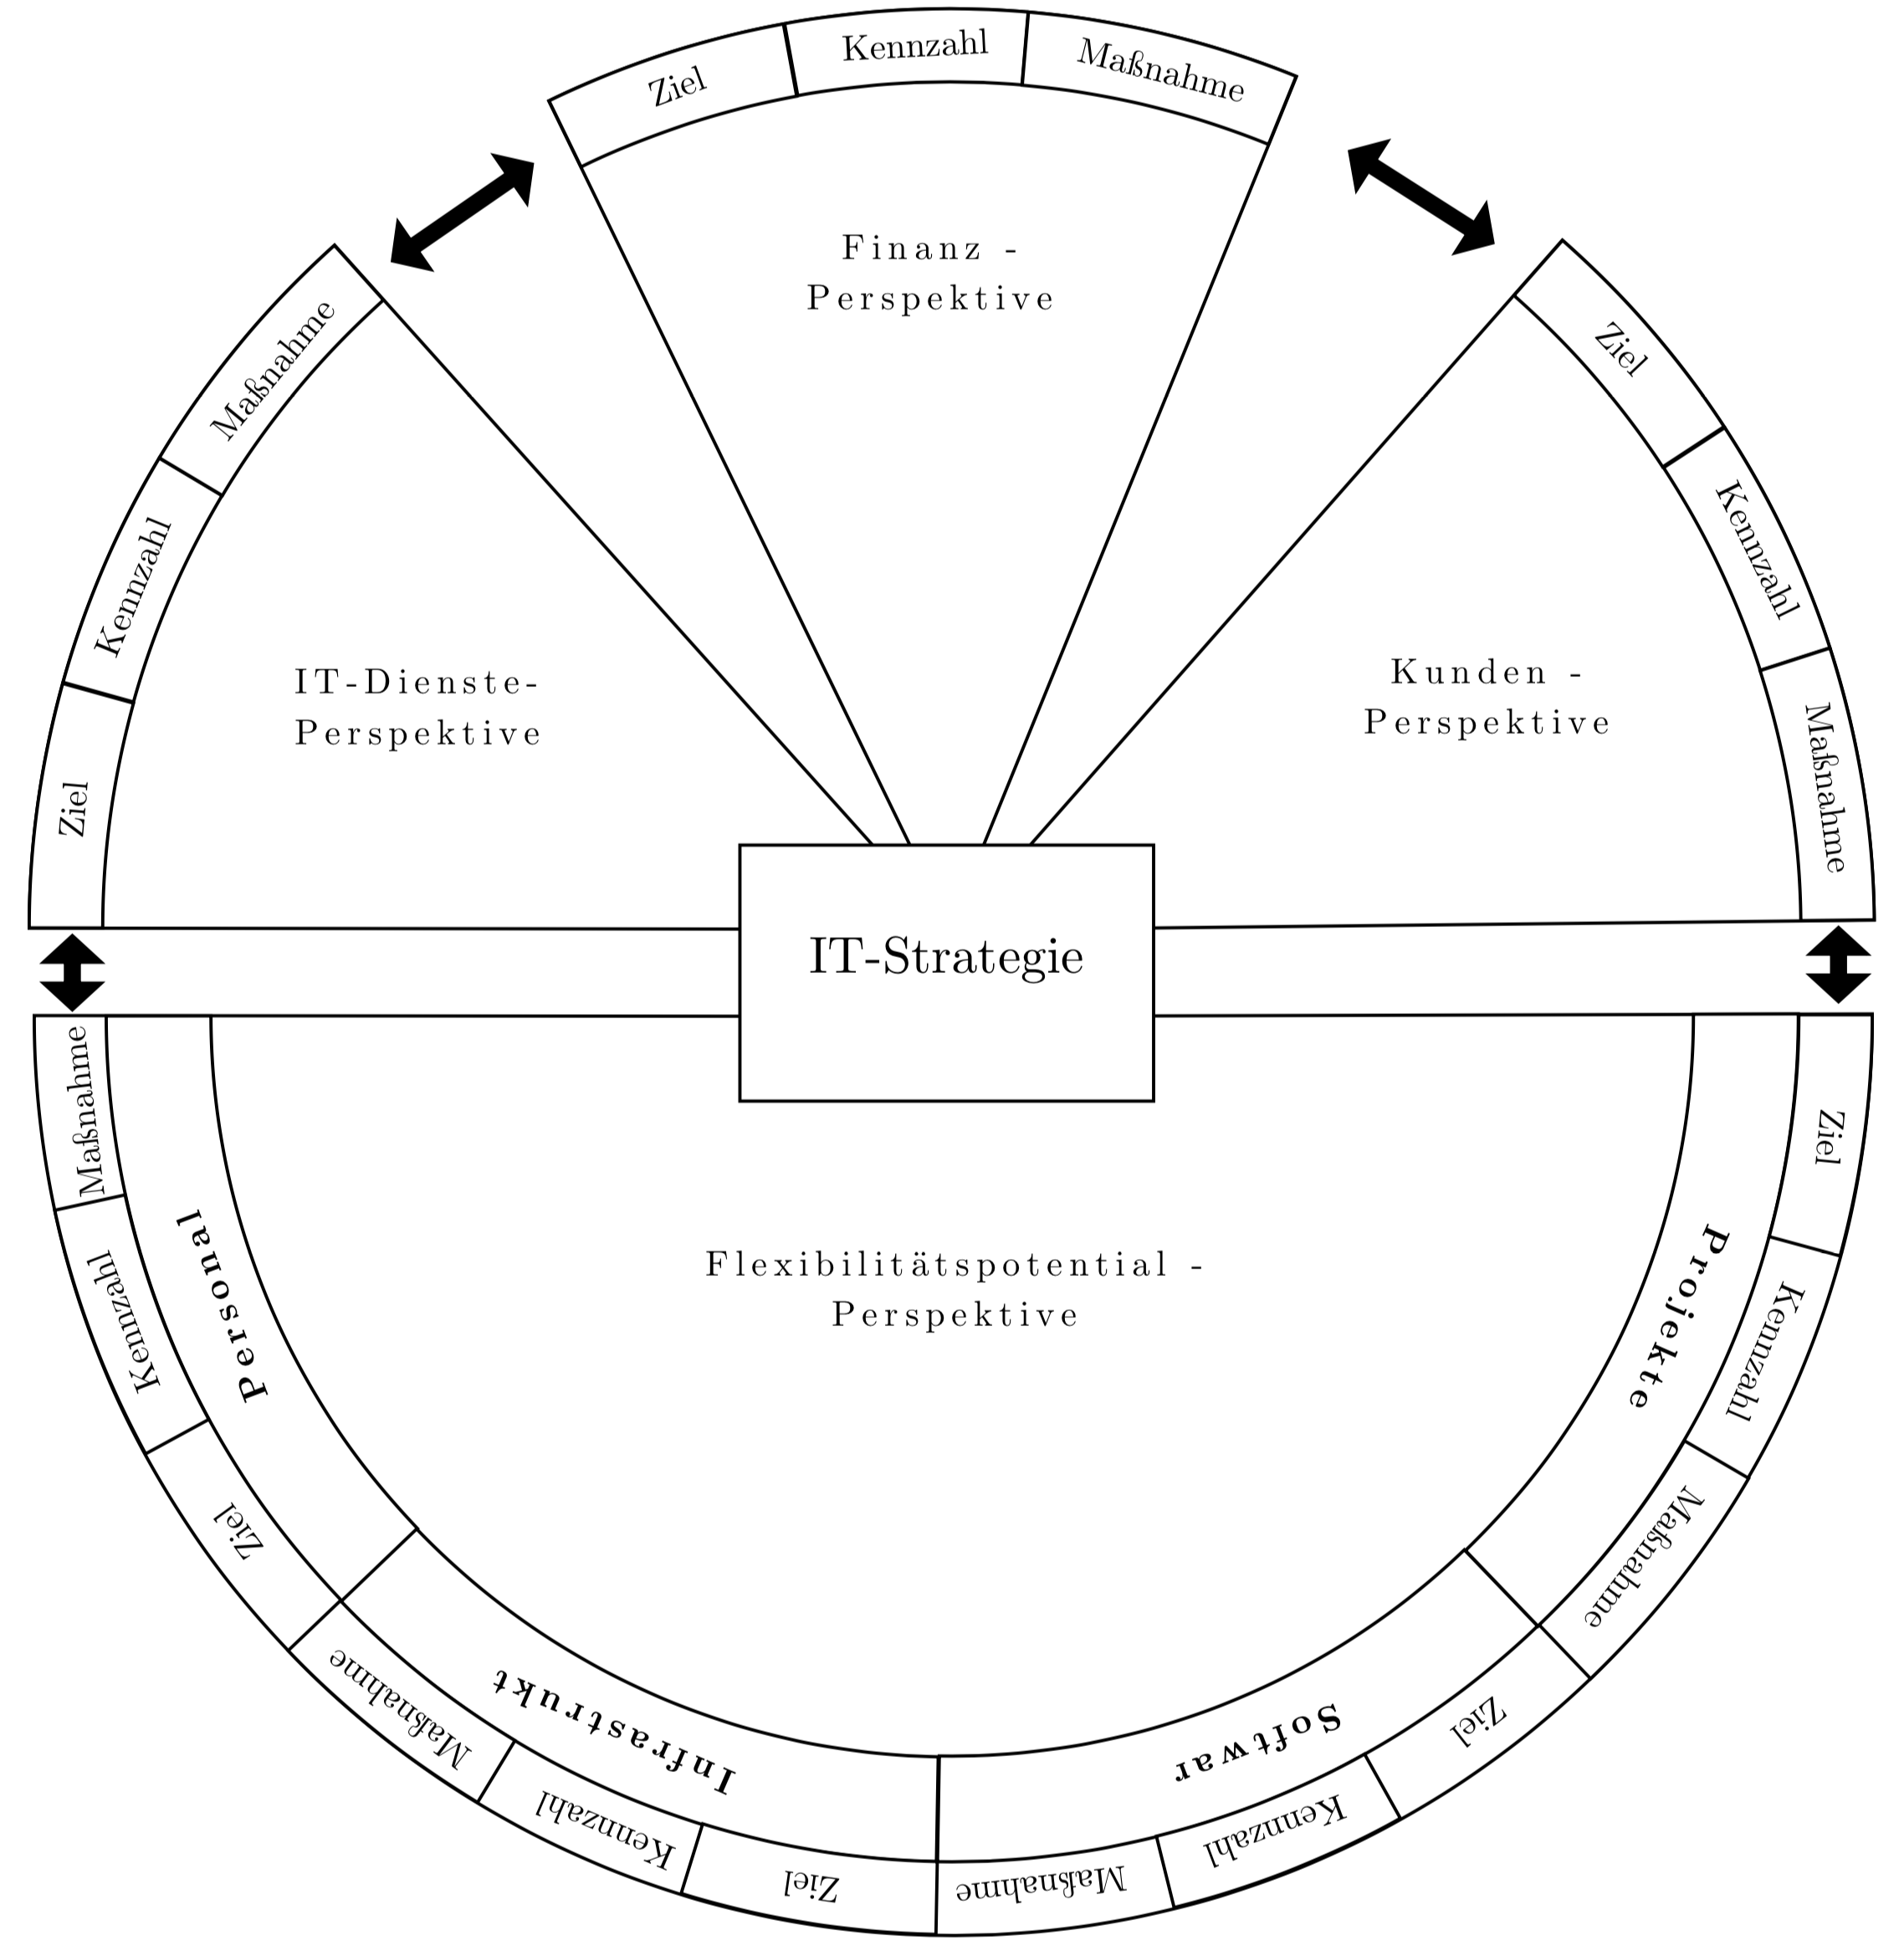
\includegraphics[width=0.75\linewidth]{flex_it}
\captionof{figure}[FlexIT]{FlexIT\footnotemark}
\label{img:flex_it}
\end{figure}
\addtocounter{footnote}{+0}\footnotetext{Eigene Darstellung in Anlehnung an}
\noindent Das Resultat, das hier nun mit der Bezeichnung \textit{FlexIT} versehen wird, kann die vorgeschlagenen Ma�nahmen wie agile Durchf�hrung von Projekten, Modularisierung der Anwendungslandschaft, Aufbau von Infrastrukturredundanz etc. steuern, indem es sie operativ begleitet und bewertet.\\
Die Ma�nahmen, f�r die auch keine ersch�pfende und allgemeing�ltige Definition vorgenommen werden kann, sind dazu vorab in einer IT-Strategie zu definieren und die  Wirkungsketten auf Kompatibilit�t zu hierarchisch �bergeordneten Zielen zu pr�fen.
Unternehmensspezifisch sind auch die jeweiligen Zielwerte der Flexibilit�tskennzahlen zu definieren, da eine vollst�ndige Implementation der Ma�nahmen wie 100\% Mobilit�t des Personals durch ausbleibende Kommunkation in B�ror�umen kontraintuitive Effekte haben kann und nicht proportional zum Implementationsgrad produktivit�tsf�rdernd wirkt.
Optimale bzw. Grenzwerte, die multifaktoriell von der Unternehmensorganisation beeinflusst werden, sind also ebenfalls unternehmensspezifisch, aber modellintern durch die dargelegten Kennzahlkombinationen zu ermitteln.
Ein diesbez�gliches Beispiel best�nde in der schrittweisen Einf�hrung von Arbeitsplatzmobilit�t f�r Teile des Personals und deren Einsatz im Homeoffice, die zun�chst zur Steigerung des verbundenen Produktivit�tsma� f�hrt und ggf. ab einem gewissen Anteil, z.B. �ber 50\% Implementationsgrad wieder r�ckl�ufige Produktivit�t erzielt, da die direkte Kommunikation zu stark gesunken ist, weshalb keine weitere Ma�nahmenimplementation mehr vorzunehmen und stattdessen 50\% als Zielwert festzusetzen w�re.\\
Eine gleichwertige Parameterkombination ist, z.B. mit den in dieser Arbeit definierten Kennzahlen, auch f�r �brige Ma�nahmen jeweils zu ermitteln und fortw�hrend die Strategie daran zu validieren.
%-Beispiel von Kennzahlensteigerung zu Wertbeitragssteigerung
%\subsection{Interpretation als Werttreiber}

\section{Fazit und Potential}
Mit Abschluss der Konzeption kann nun die Zielerreichung �berpr�ft, die Ergebnisqualit�t und -bedeutung diskutiert sowie ein Blick auf darauf aufbauende M�glichkeiten geworfen werden.\\\\
Das Ziel, Flexibilit�t in der IT bewertbar und steuerbar zu machen, ist insofern erreicht, als dass das konzeptionelle Ergebnis die in \ref{sec:aufgabenundziele} aufgestellten Ergebniskriterien erf�llt:
Das in Form einer \gls{BSC} entworfene Resultat zentriert Informationen zur Steuerung von Ma�nahmen unterschiedlichen zeitlichen Horizonts.
Die Ma�nahmen, die dabei die Flexibilisierung interner Verh�ltnisse anvisieren, um auf eine komplexe und dynamische Umwelt reagieren zu k�nnen, entsprechen insoweit der Controlling-Konzeption von K�pper et al. und Horv\'ath et al., als dass deren ebenda dargestellte Anspr�che ber�cksichtigt sind.\\
Die modellierten Verbindungen zu gesamtunternehmerischen Zielen der Kunden- und Finanzperspektiven lassen letztendlich sogar die Vermutung einer ganzheitlich m�glichen Steuerung zu.
Die Flexibilisierbarkeit entscheidender IT-Inhalte und deren Tragweite indizieren, dass eine konsequente Flexibilisierung �ber den Ideen-Ursprung hinaus essentielle Bestandteile einer IT-Strategie abdecken kann.
%\\
�ber die Flexibilisierung sind letztendlich nicht nur die die Flexibilit�tspotentiale zur Beherrschung der dynamischen Umwelt zu schaffen, sondern auch z.B. personelle Produktivit�tsverbesserungen oder h�heres Business Alignment zu realisieren.
Dementsprechend bestehen M�glichkeiten zur Aussch�pfung unterschiedlicher positiver Effekte, z.B. monet�rer oder qualitativer Natur.
\\
\\ 
Ein diesbez�glicher empirischer Beweis an Realobjekten zur Validierung des Modells steht allerdings aus, weshalb nur Analogien zu Erkenntnissen �hnlicher Forschung ermittelt und zur qualitativen Validierung herangezogen werden k�nnen.
Hierzu w�re z.B. die Untersuchung von Byrd/Turner zu gesamtsystemischen Flexibilit�ts-Indikatoren (Integration, Konnektivit�t, Modularit�t)\footnote{Vgl. \cite{byrdturner2000}.} zu nennen, die Unternehmenserfolg tats�chlich in Abh�ngigkeit von diesen nachweisen konnten.\footnote{Vgl. \cite[S.49-50]{byrdturner2001}.}
Die Definition und Zustandsermittlung war dabei allerdings nicht durchgehend strikt und konnte nur teilweise eine vergleichsf�hige Implementationsstrategie aufzeigen.
\\
Die empirische Validierung m�sste also in hierauf aufbauenden Forschungsbeitr�gen durchgef�hrt werden.
\textit{FlexIT} erm�glicht allerdings unternehmens�bergreifende Vergleichbarkeit von Flexibilit�t und deren Auswirkungen und ist dahingehend modellinh�rent validierbar.
In dieser Hinsicht ist das Modell auch bisherigen Flexibilit�tsuntersuchungen in der IT insoweit voraus, als dass z.B. die nicht eindeutig messbaren, zumal nicht eindeutig definierten, Indikatoren von Byrd/Turner nicht unternehmens�bergreifend und nicht im Detail, d.h. je Ma�nahme, sondern nur in Verbindung validierbar sind.
Gleichwohl l�sst die Einstufung der Verbindung zum Unternehmenserfolg, die in qualitativer Erhebung damit erbracht wurde\footnote{Vgl. \cite{Tallon20030UF}.}, den Schluss zu, dass der ganzheitliche Steuerungsansatz, der in dieser Arbeit konzipiert ist, einen validen Zugang darstellt und die durch Flexibilit�t angestrebten Ziele die vermutete Tragweise besitzen k�nnen.
\\
\\
Nichtsdestotrotz bestehen im Modell Gestaltungsm�glichkeiten.
Die Flexibilit�tsans�tze aus dem \gls{L-C} z.B., die mit denen des \gls{P-C} in Verbindung stehen (vgl. \ref{bsc_quellen}), weisen ggf. auch Adaptionspotential auf und k�nnen andere Messungsans�tze liefern.
Auch die Dimensionsdefinition ist nicht zwingend vollst�ndig, sodass in Modellen �hnlich dem bereichsklassifizierenden Identifikationsansatz unter Umst�nden weitere Dimensionen zu entdecken sind.
Sofern in anderen Dimensionen, z.B. auch durch andere Methodenadaptionen, also wirkungsrelevante Aspekte zu ermitteln sind, k�nnten Dimensionen erg�nzt oder substituiert werden.
Je nach L�nge der entstehenden Wirkungsketten w�re hier allerdings darauf zu achten, dass schwach kausale Abh�ngigkeiten die Erfolgswirkung verw�ssern k�nnen.
Eine Fortf�hrung des Modells durch Dimensionserg�nzungen ist insofern also nicht zwingend eine Verbesserung, wenn sie Wirkungszusammenh�nge in der Folge zu weitreichend auslegt.
\\
Auch innerhalb der in dieser Arbeit beschriebenen Dimensionen besteht inhaltliches Erg�nzungspotential hinsichtlich der Flexibilisierungsma�nahmen, Messungsans�tze sowie Wertbeitragsermittlungsmethoden, die in deren jeweiligen Fachspezifika, also z.B. innerhalb der Dimension Personal zu suchen w�ren.
Dies kann als unternehmensspezifische Adaption oder Modellerweiterung verfolgt werden, betont jedoch abseits der Umsetzung den abstrakten Charakter des entworfenen Modells.
\\
Die postulierten Erweiterungs- und Anpassungsoptionen bestehen also in vertikaler und horizontaler Richtung.
\\\\
F�r die Flexibilit�t der IT-Organisation ist letztlich zu konstatieren, dass die Betrachtung weder in der Breite noch der Tiefe stattgefunden hat wie f�r produktionswirtschaftliche Flexibilit�t, die trotzdem noch nicht zu allgemeinem Konsens gelangt ist.
Auch f�r die IT ist daher in Anbetracht der f�r sie ebenfalls geltenden dynamischen Umweltbedingungen anzunehmen, dass die Diskussion um Flexibilit�t �hnliche Ausma�e annehmen kann und vielleicht auch sollte.\\
Diese Arbeit leistet dazu einen konzeptionellen Beitrag.
%\todo{anwendungsorientiert, geht aber sicher auch hart akademisch}
%Multiprojektcontrolling einbeziehen
%auf logistikcontrolling eingehen

\newpage
\backmatter
\addcontentsline{toc}{section}{Quellenverzeichnis}
\printbibliography
\appendix
\addcontentsline{toc}{section}{Anhang}
\renewcommand\thesection{\Alph{section}}
  \begin{appendix}
  \let\svaddcontentsline\addcontentsline
\renewcommand\addcontentsline[3]{%
  \ifthenelse{\equal{#1}{lof}}{}%
  {\ifthenelse{\equal{#1}{lot}}{}{\svaddcontentsline{#1}{#2}{#3}}}}
 \renewcommand\thefigure{\thesubsection.\arabic{figure}}  
  \setcounter{figure}{0}

\section*{Anhang}  
  \section{Einsatzbereiche nach Gottmann}
  \subsection{Beschaffung/Lieferanten}\label{a1}
    \begin{figure}[!htb]
	\centering
	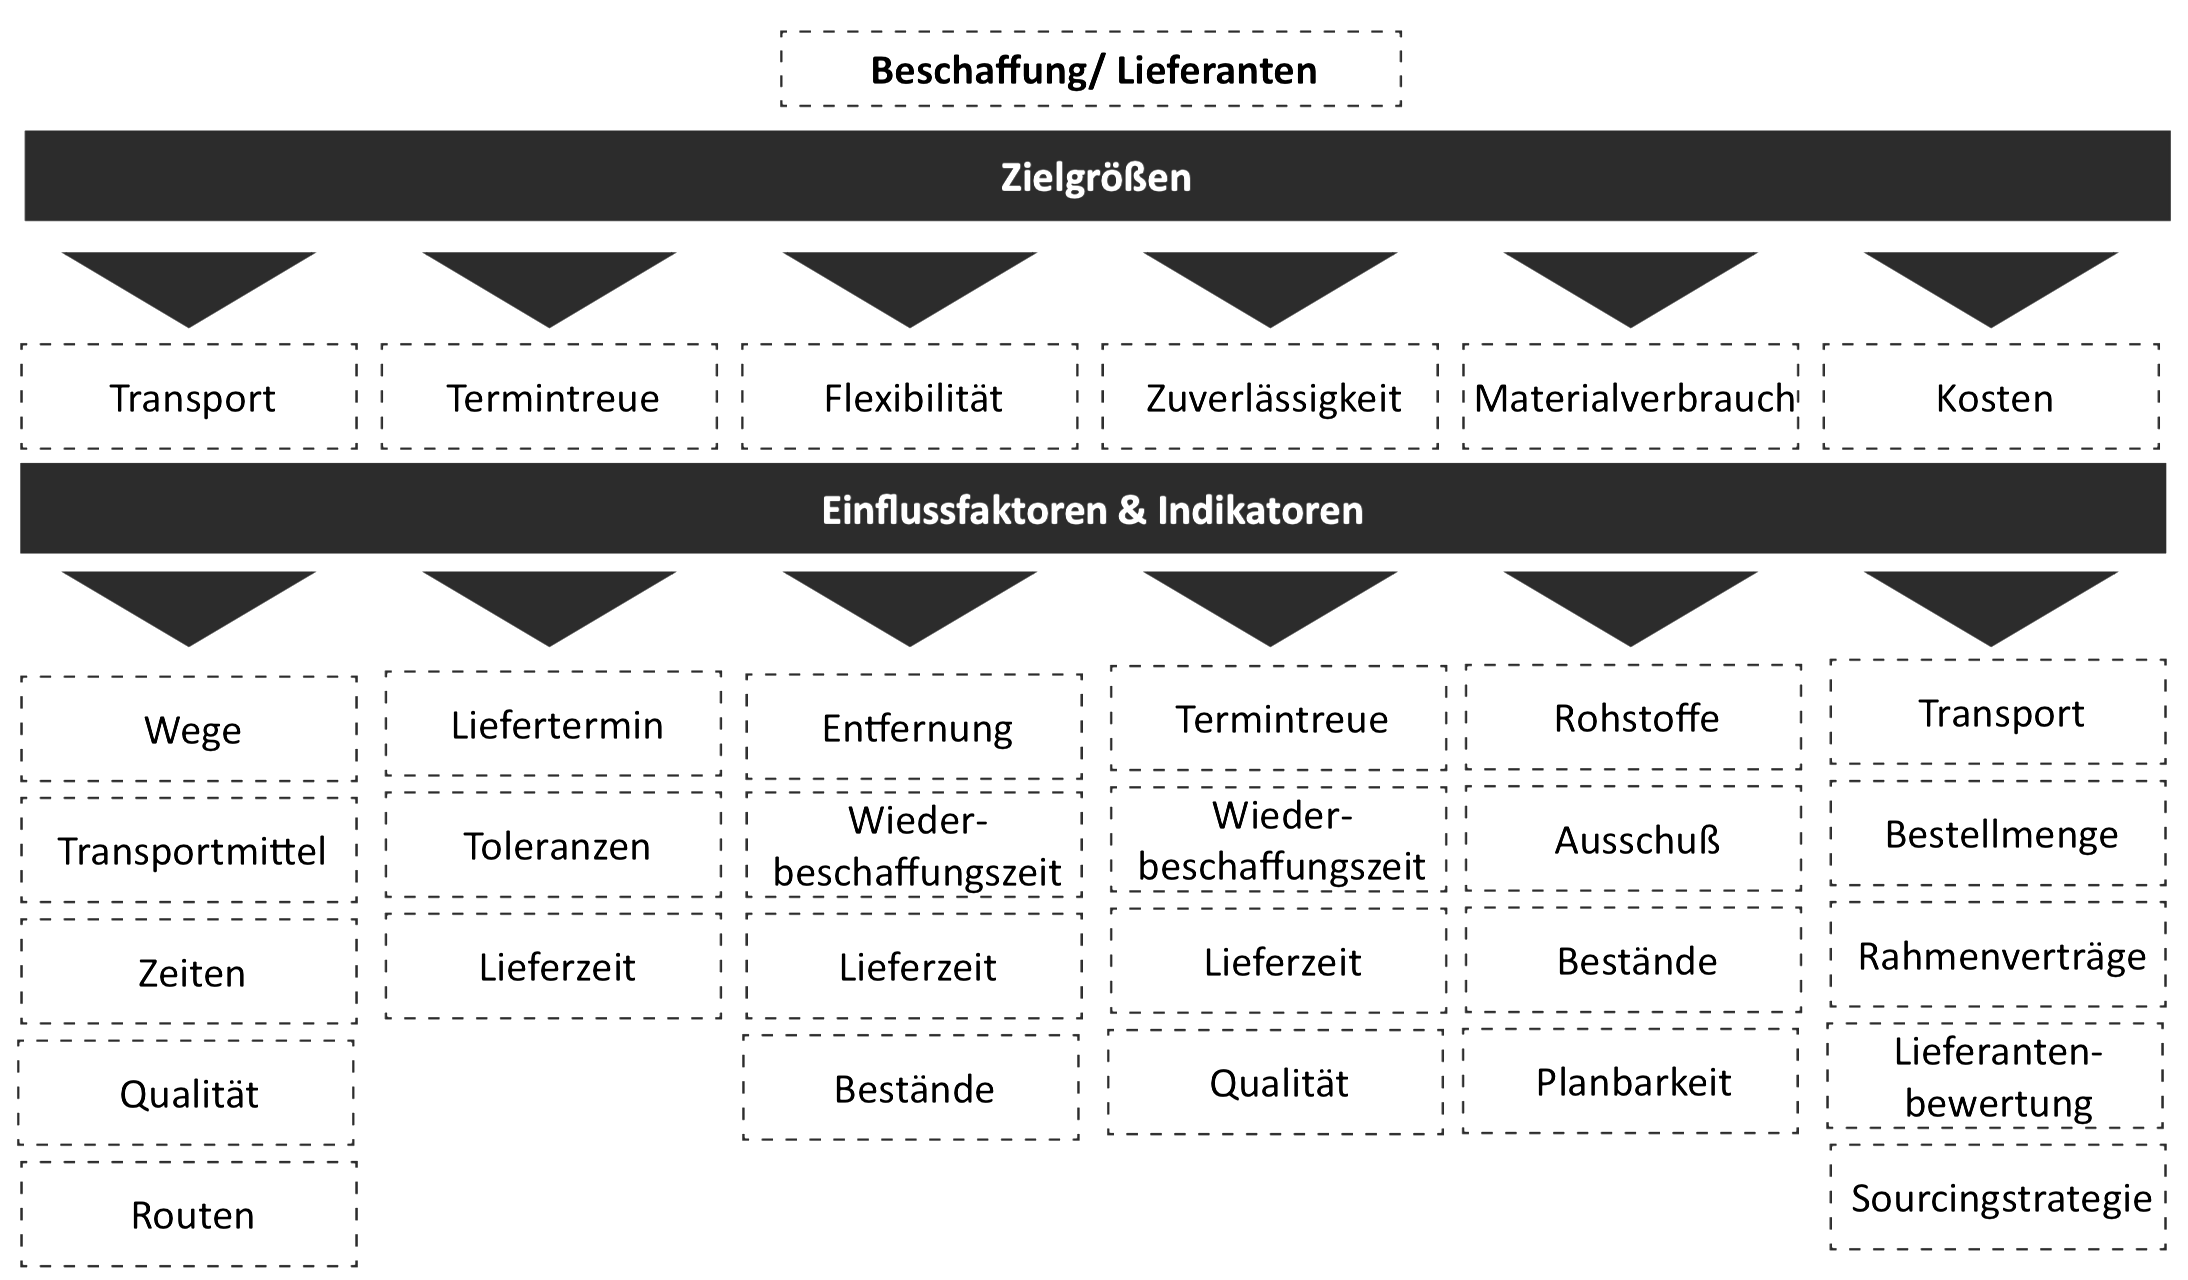
\includegraphics[width=0.7\linewidth]{gottmann_1}
	\captionof{figure}[Zielgr��en, Einflussfaktoren und Indikatoren in der Beschaffung]{Zielgr��en, Einflussfaktoren und Indikatoren in der Beschaffung\footnotemark}
	\label{img:gottmann_1}
	\end{figure}
	\addtocounter{footnote}{+0}\footnotetext{\cite[Abb. 3.5]{Gottmann2019}}
	
  \subsection{Anlagen und Produktionsprozesse}\label{a2}
    \begin{figure}[!htb]
	\centering
	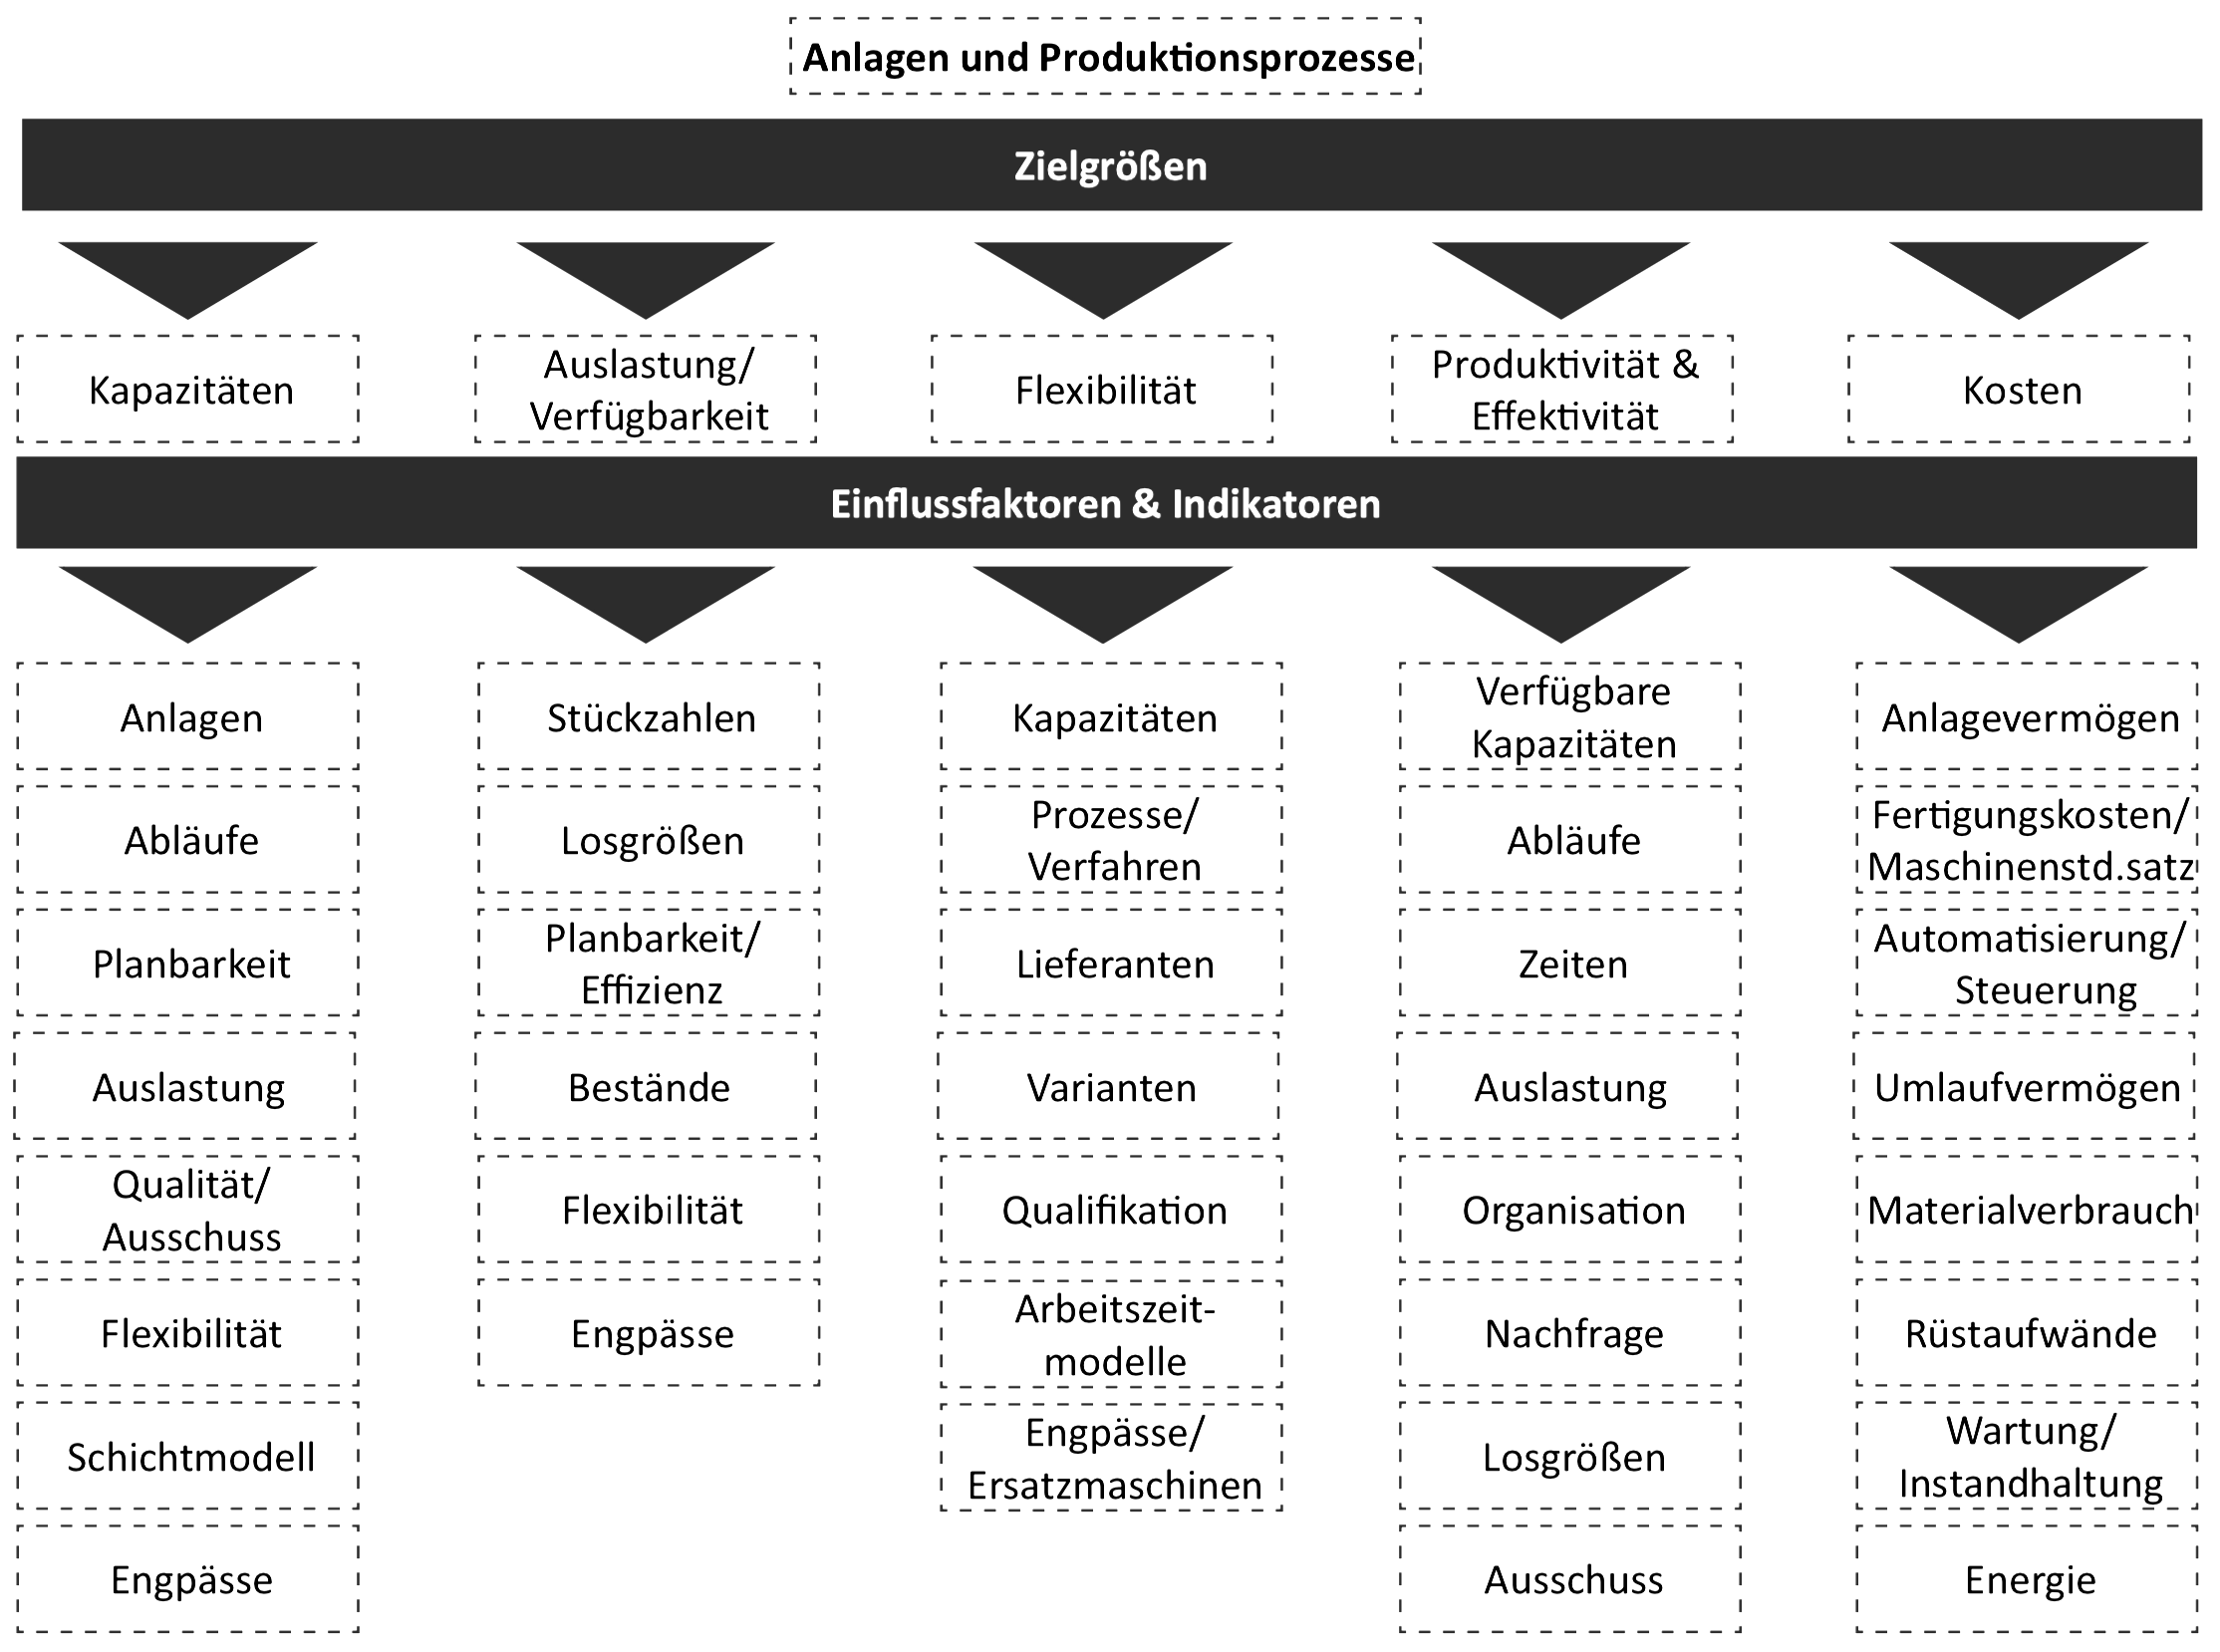
\includegraphics[width=0.7\linewidth]{gottmann_2}
	\captionof{figure}[Zielgr��en, Einflussfaktoren und Indikatoren f�r Anlagen und Produktionsprozesse]{Zielgr��en, Einflussfaktoren und Indikatoren f�r Anlagen und Produktionsprozesse\footnotemark}
	\label{img:gottmann_2}
	\end{figure}
	\addtocounter{footnote}{+0}\footnotetext{\cite[Abb. 3.6]{Gottmann2019}}
	\newpage

  \subsection{Personal}\label{a3}
    \begin{figure}[!htb]
	\centering
	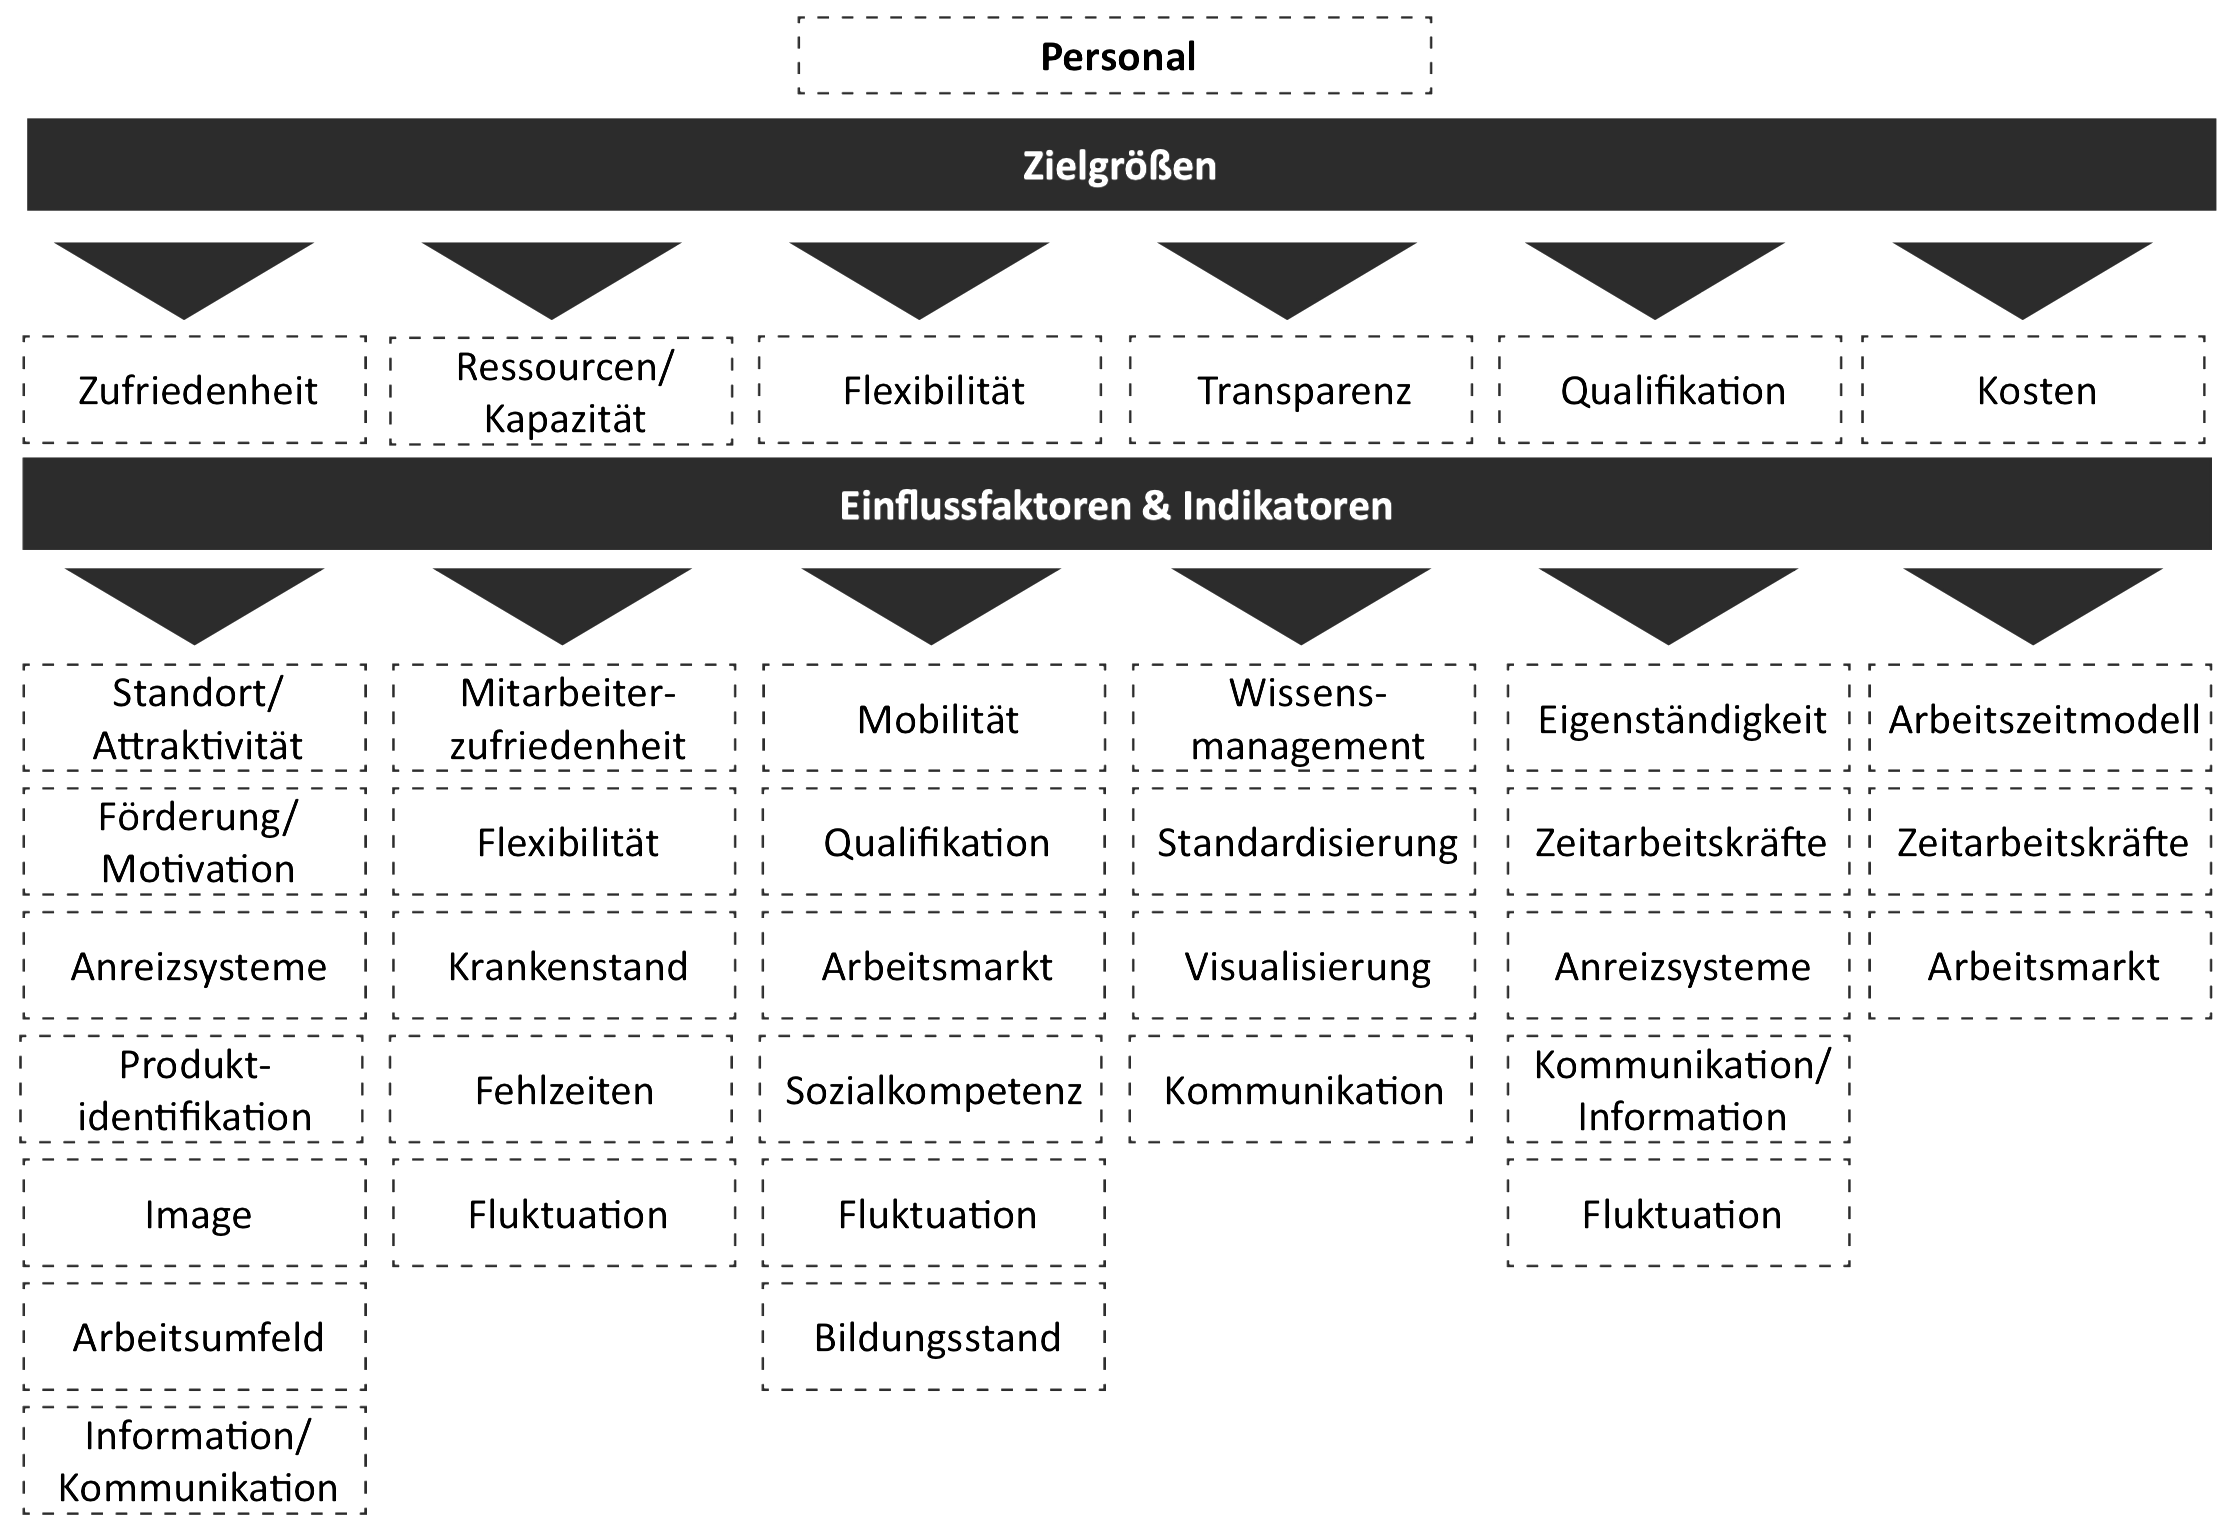
\includegraphics[width=0.8\linewidth]{gottmann_3}
	\captionof{figure}[Zielgr��en, Einflussfaktoren und Indikatoren f�r Personal]{Zielgr��en, Einflussfaktoren und Indikatoren f�r Personal\footnotemark}
	\label{img:gottmann_3}
	\end{figure}
	\addtocounter{footnote}{+0}\footnotetext{\cite[Abb. 3.7]{Gottmann2019}}
	
  \subsection{Qualit�t}\label{a4}
    \begin{figure}[!htb]
	\centering
	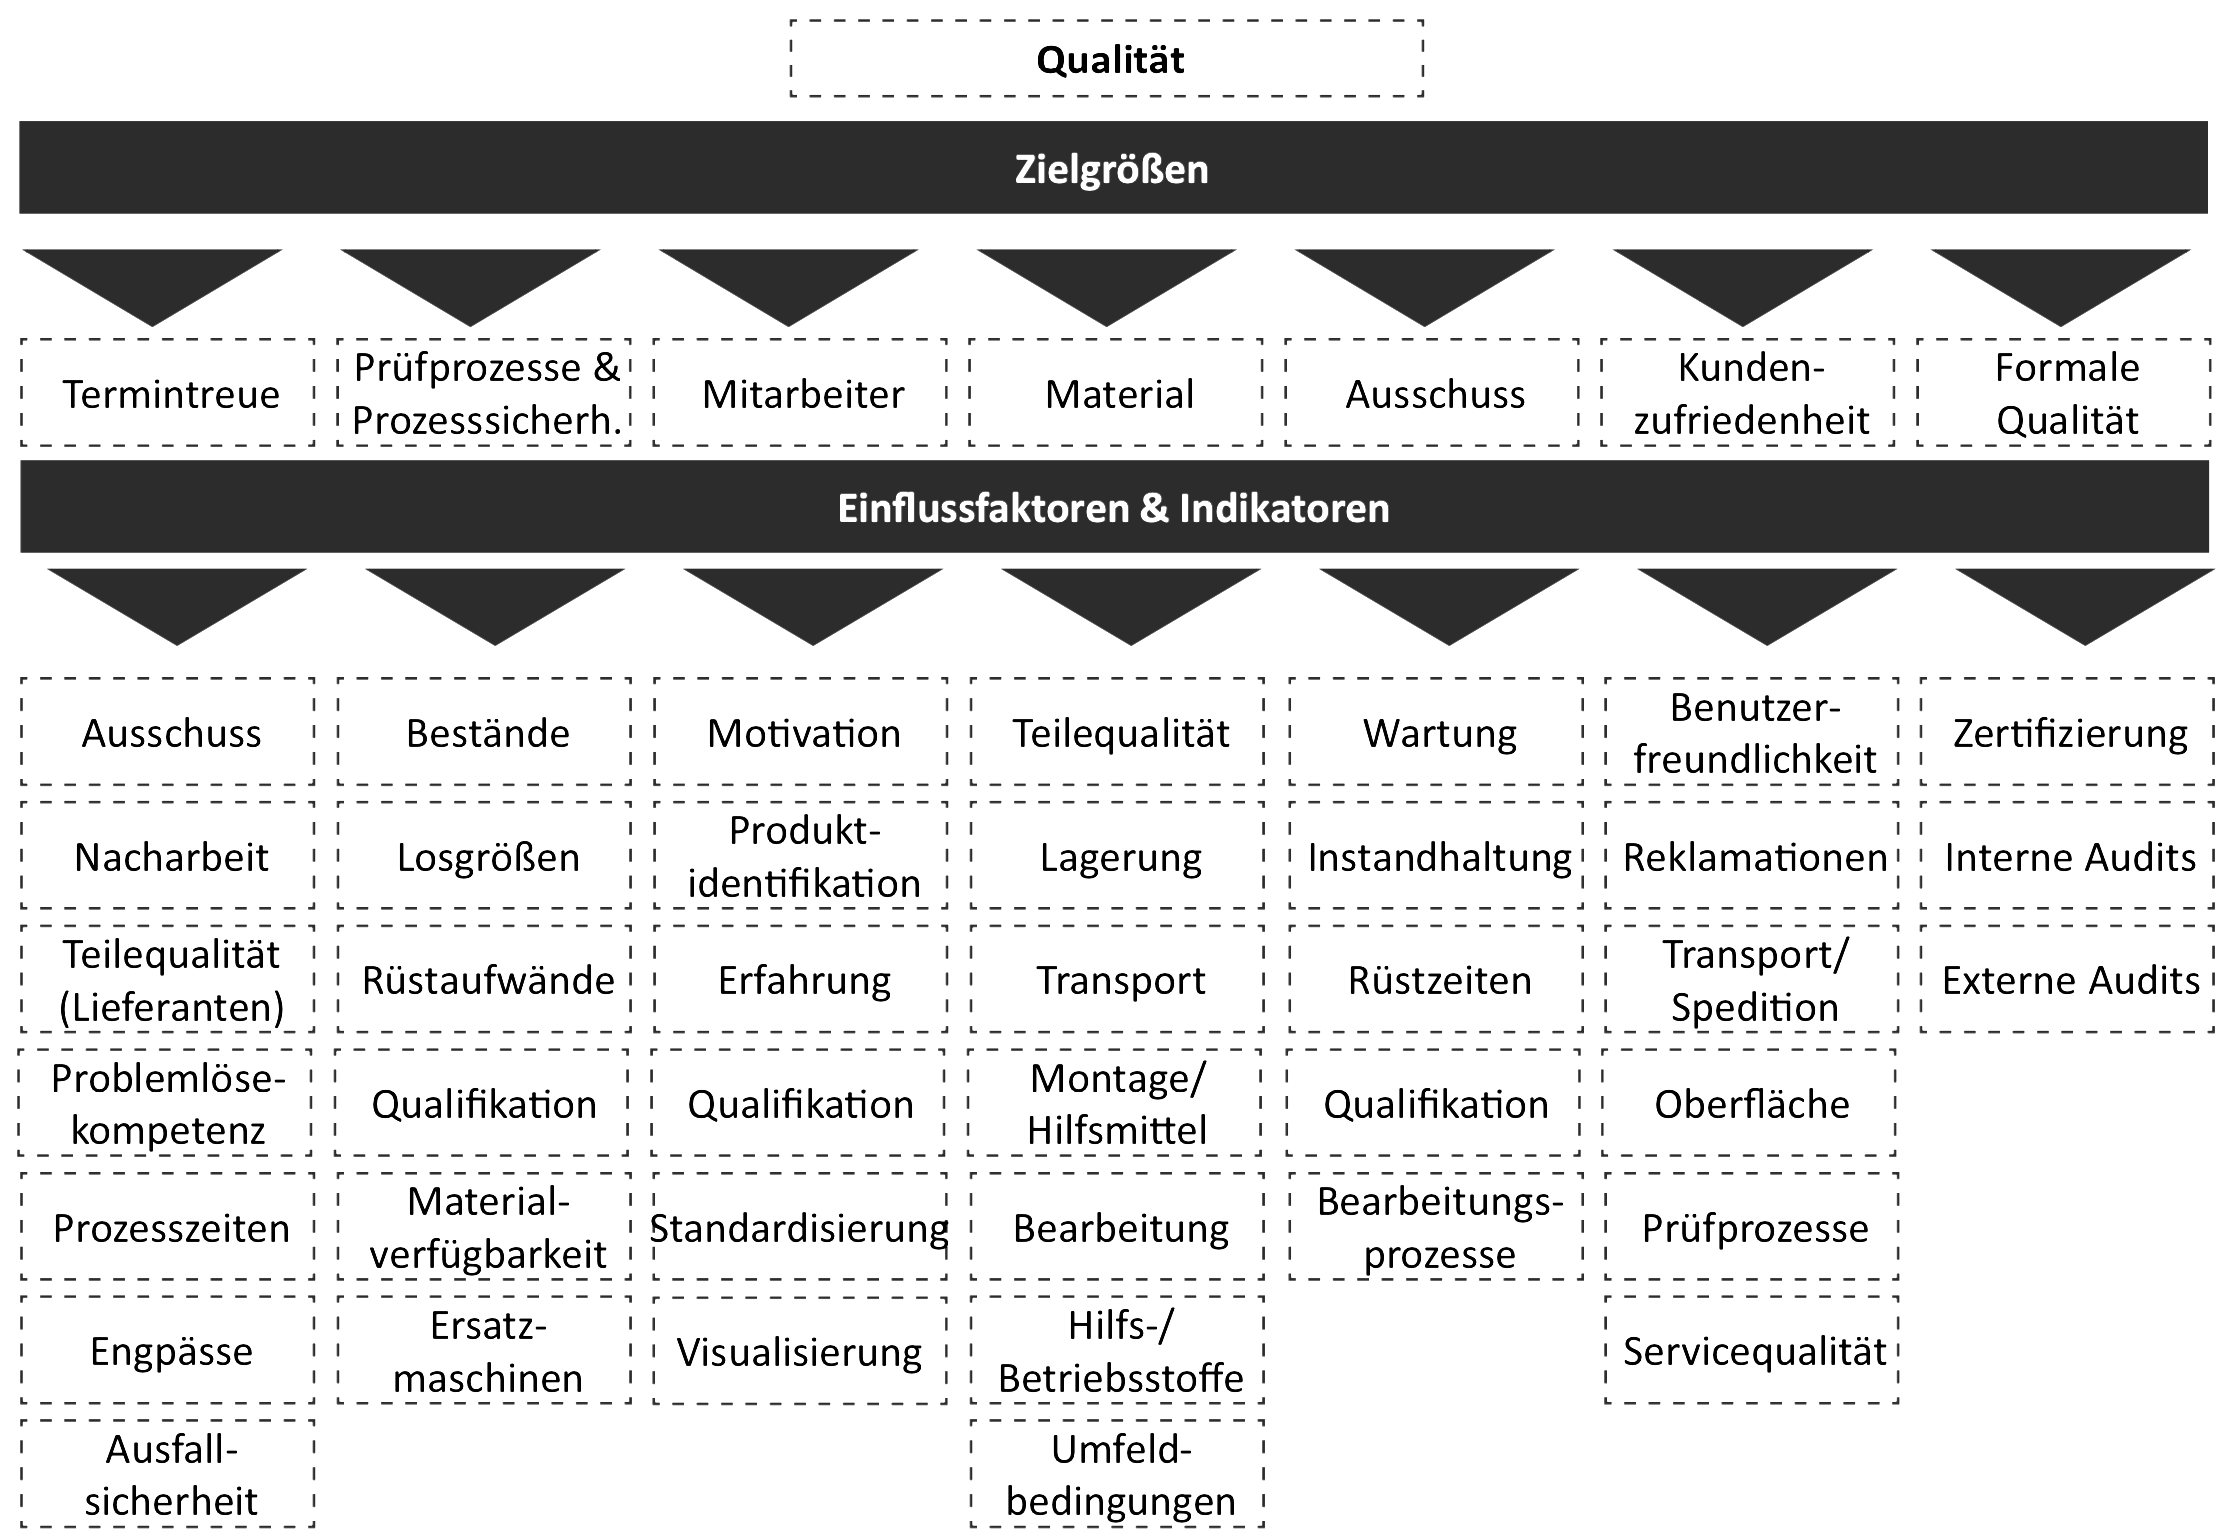
\includegraphics[width=0.8\linewidth]{gottmann_4}
	\captionof{figure}[Zielgr��en, Einflussfaktoren und Indikatoren in der Qualit�t]{Zielgr��en, Einflussfaktoren und Indikatoren in der Qualit�t\footnotemark}
	\label{img:gottmann_4}
	\end{figure}
	\addtocounter{footnote}{+0}\footnotetext{\cite[Abb. 3.8]{Gottmann2019}}
	\newpage
	
  \subsection{Material und Logistik}\label{a5}
    \begin{figure}[!htb]
	\centering
	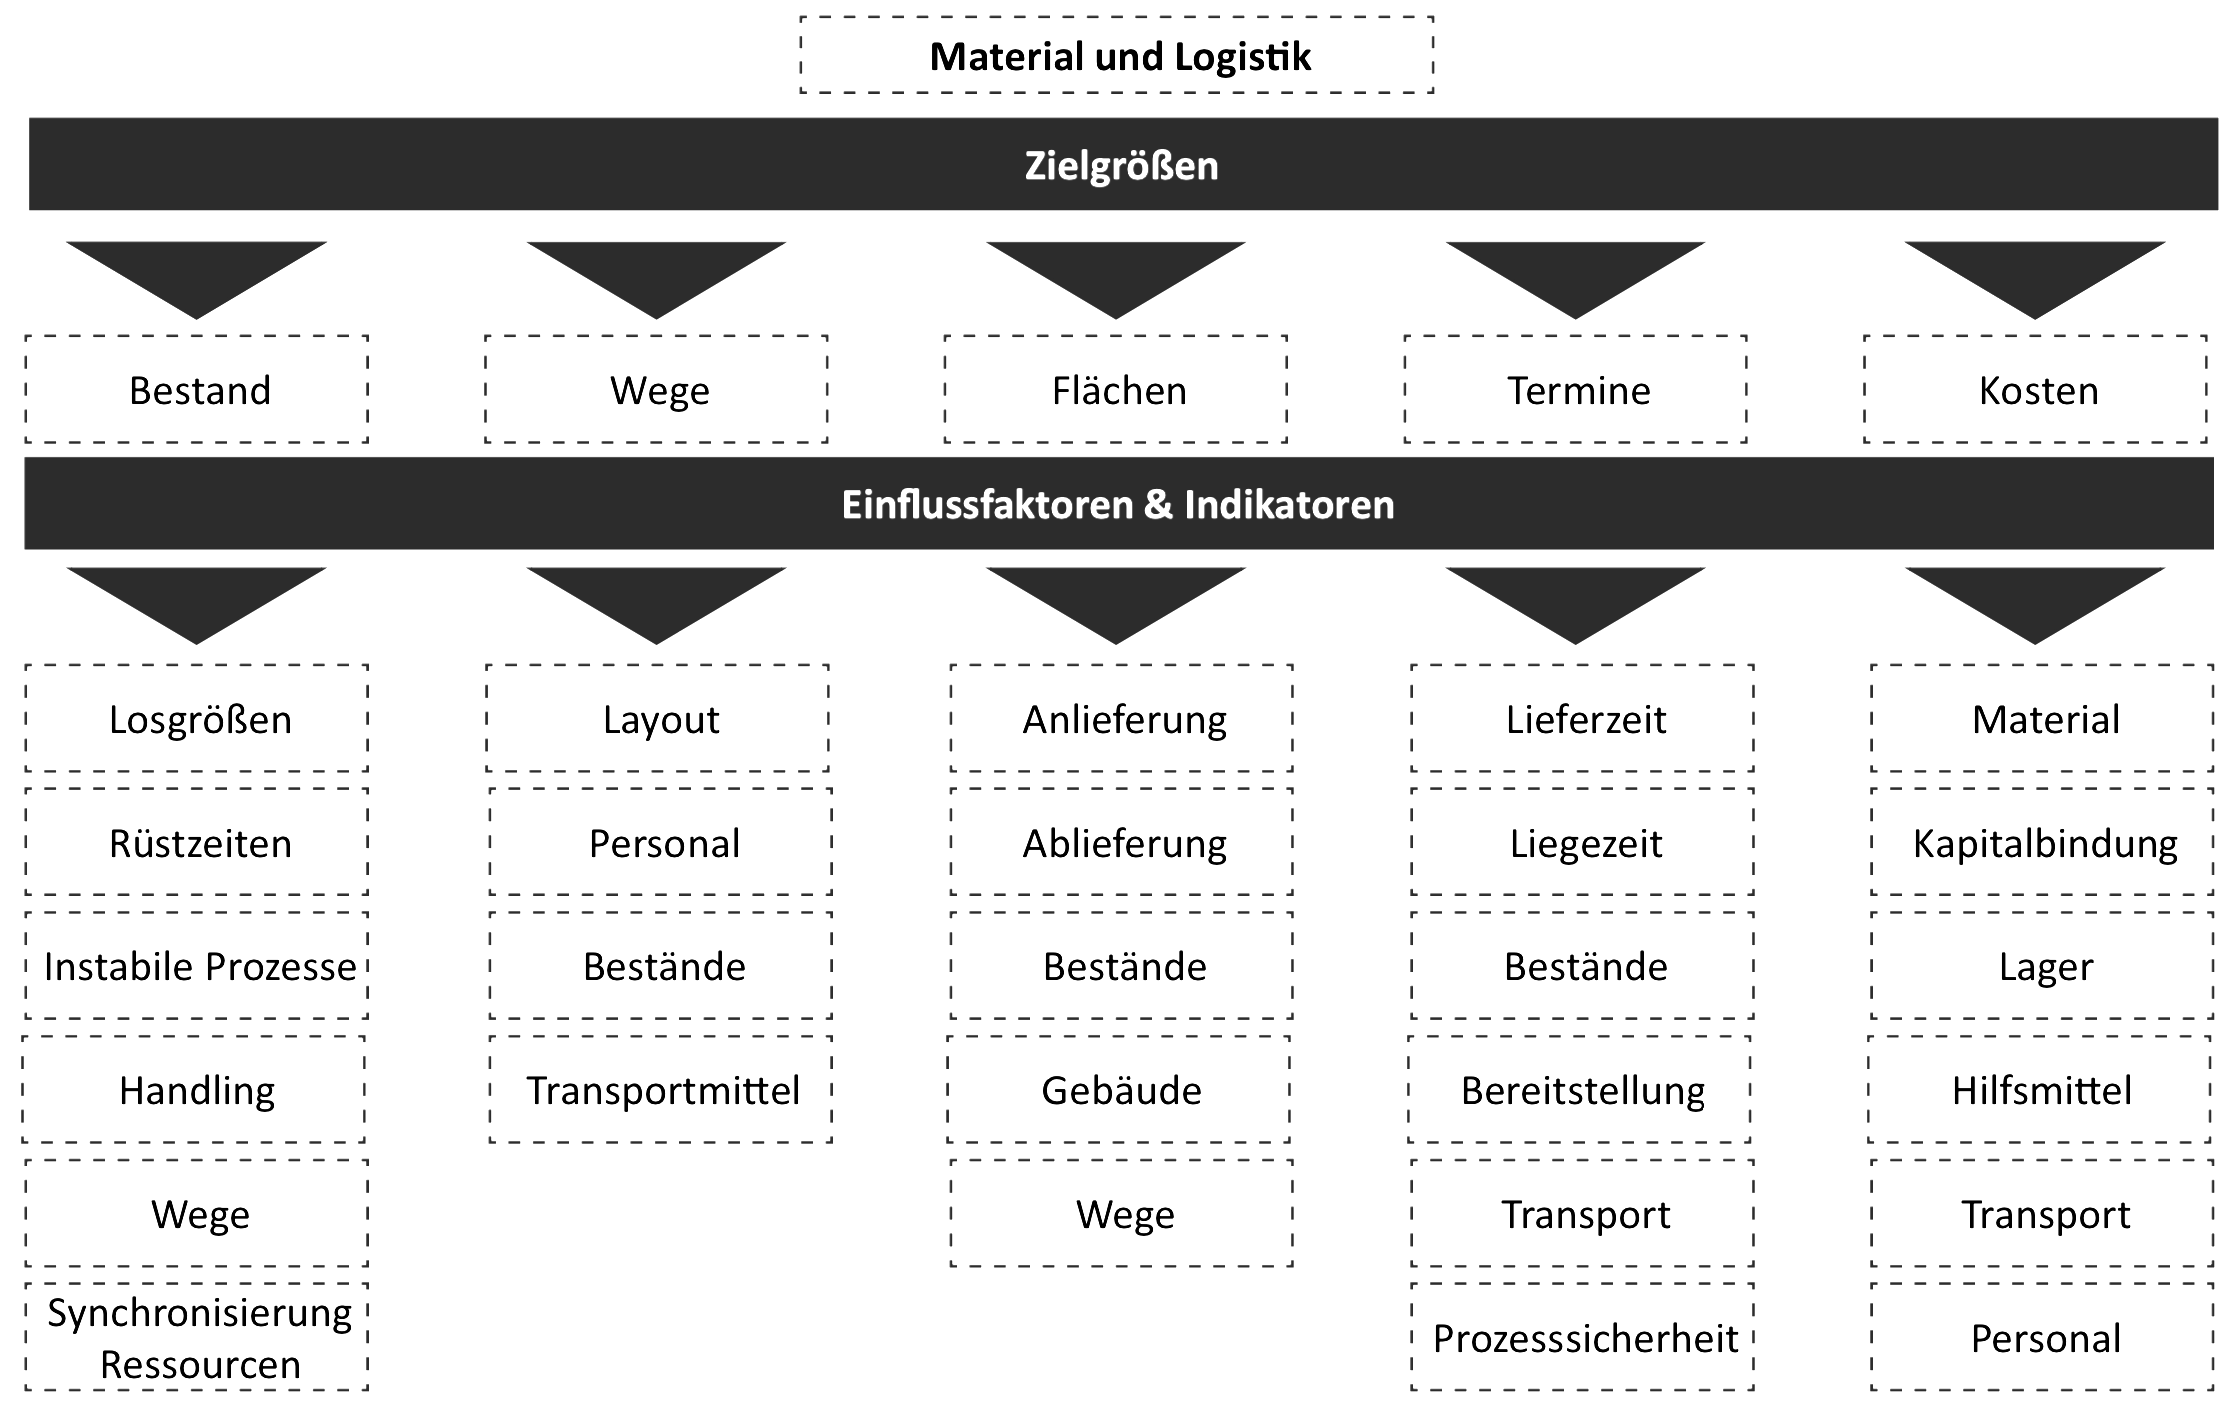
\includegraphics[width=0.8\linewidth]{gottmann_5}
	\captionof{figure}[Zielgr��en, Einflussfaktoren und Indikatoren in der Logistik]{Zielgr��en, Einflussfaktoren und Indikatoren in der Logistik\footnotemark}
	\label{img:gottmann_5}
	\end{figure}
	\addtocounter{footnote}{+0}\footnotetext{\cite[Abb. 3.9]{Gottmann2019}}
	
	 \subsection{Organisation/Auftragsabwicklung}\label{a6}
    \begin{figure}[!htb]
	\centering
	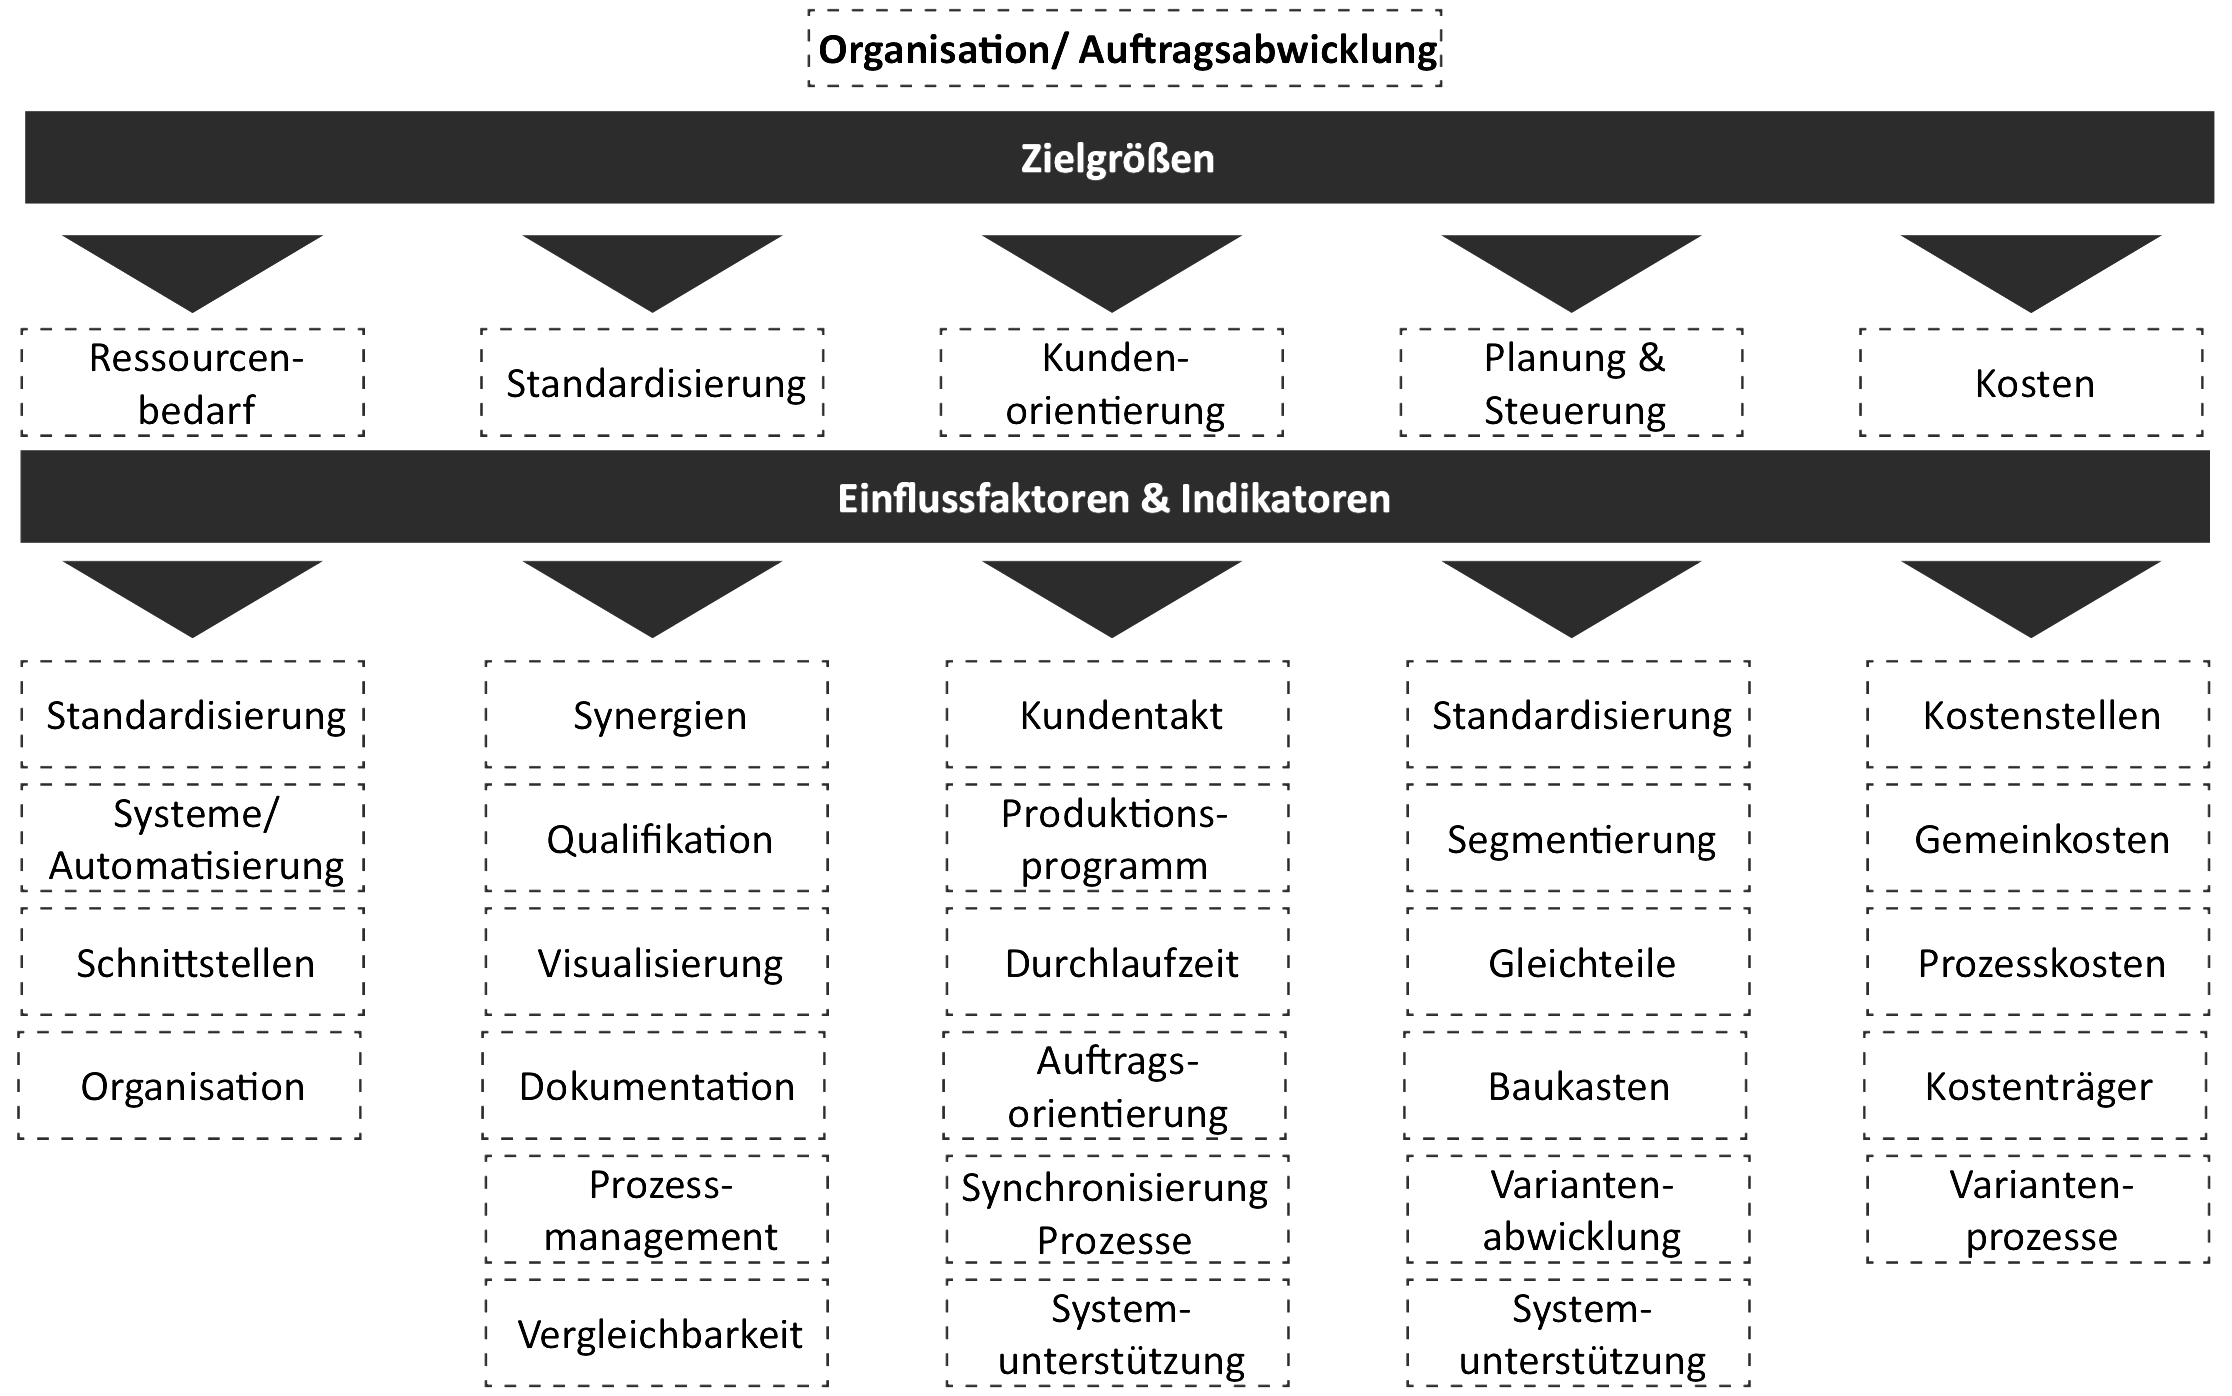
\includegraphics[width=0.8\linewidth]{gottmann_6}
	\captionof{figure}[Zielgr��en, Einflussfaktoren und Indikatoren in der Organisation]{Zielgr��en, Einflussfaktoren und Indikatoren in der Organisation\footnotemark}
	\label{img:gottmann_6}
	\end{figure}
	\addtocounter{footnote}{+0}\footnotetext{\cite[Abb. 3.10]{Gottmann2019}}
	\newpage

  \subsection{Kunden}\label{a7}
    \begin{figure}[!htb]
	\centering
	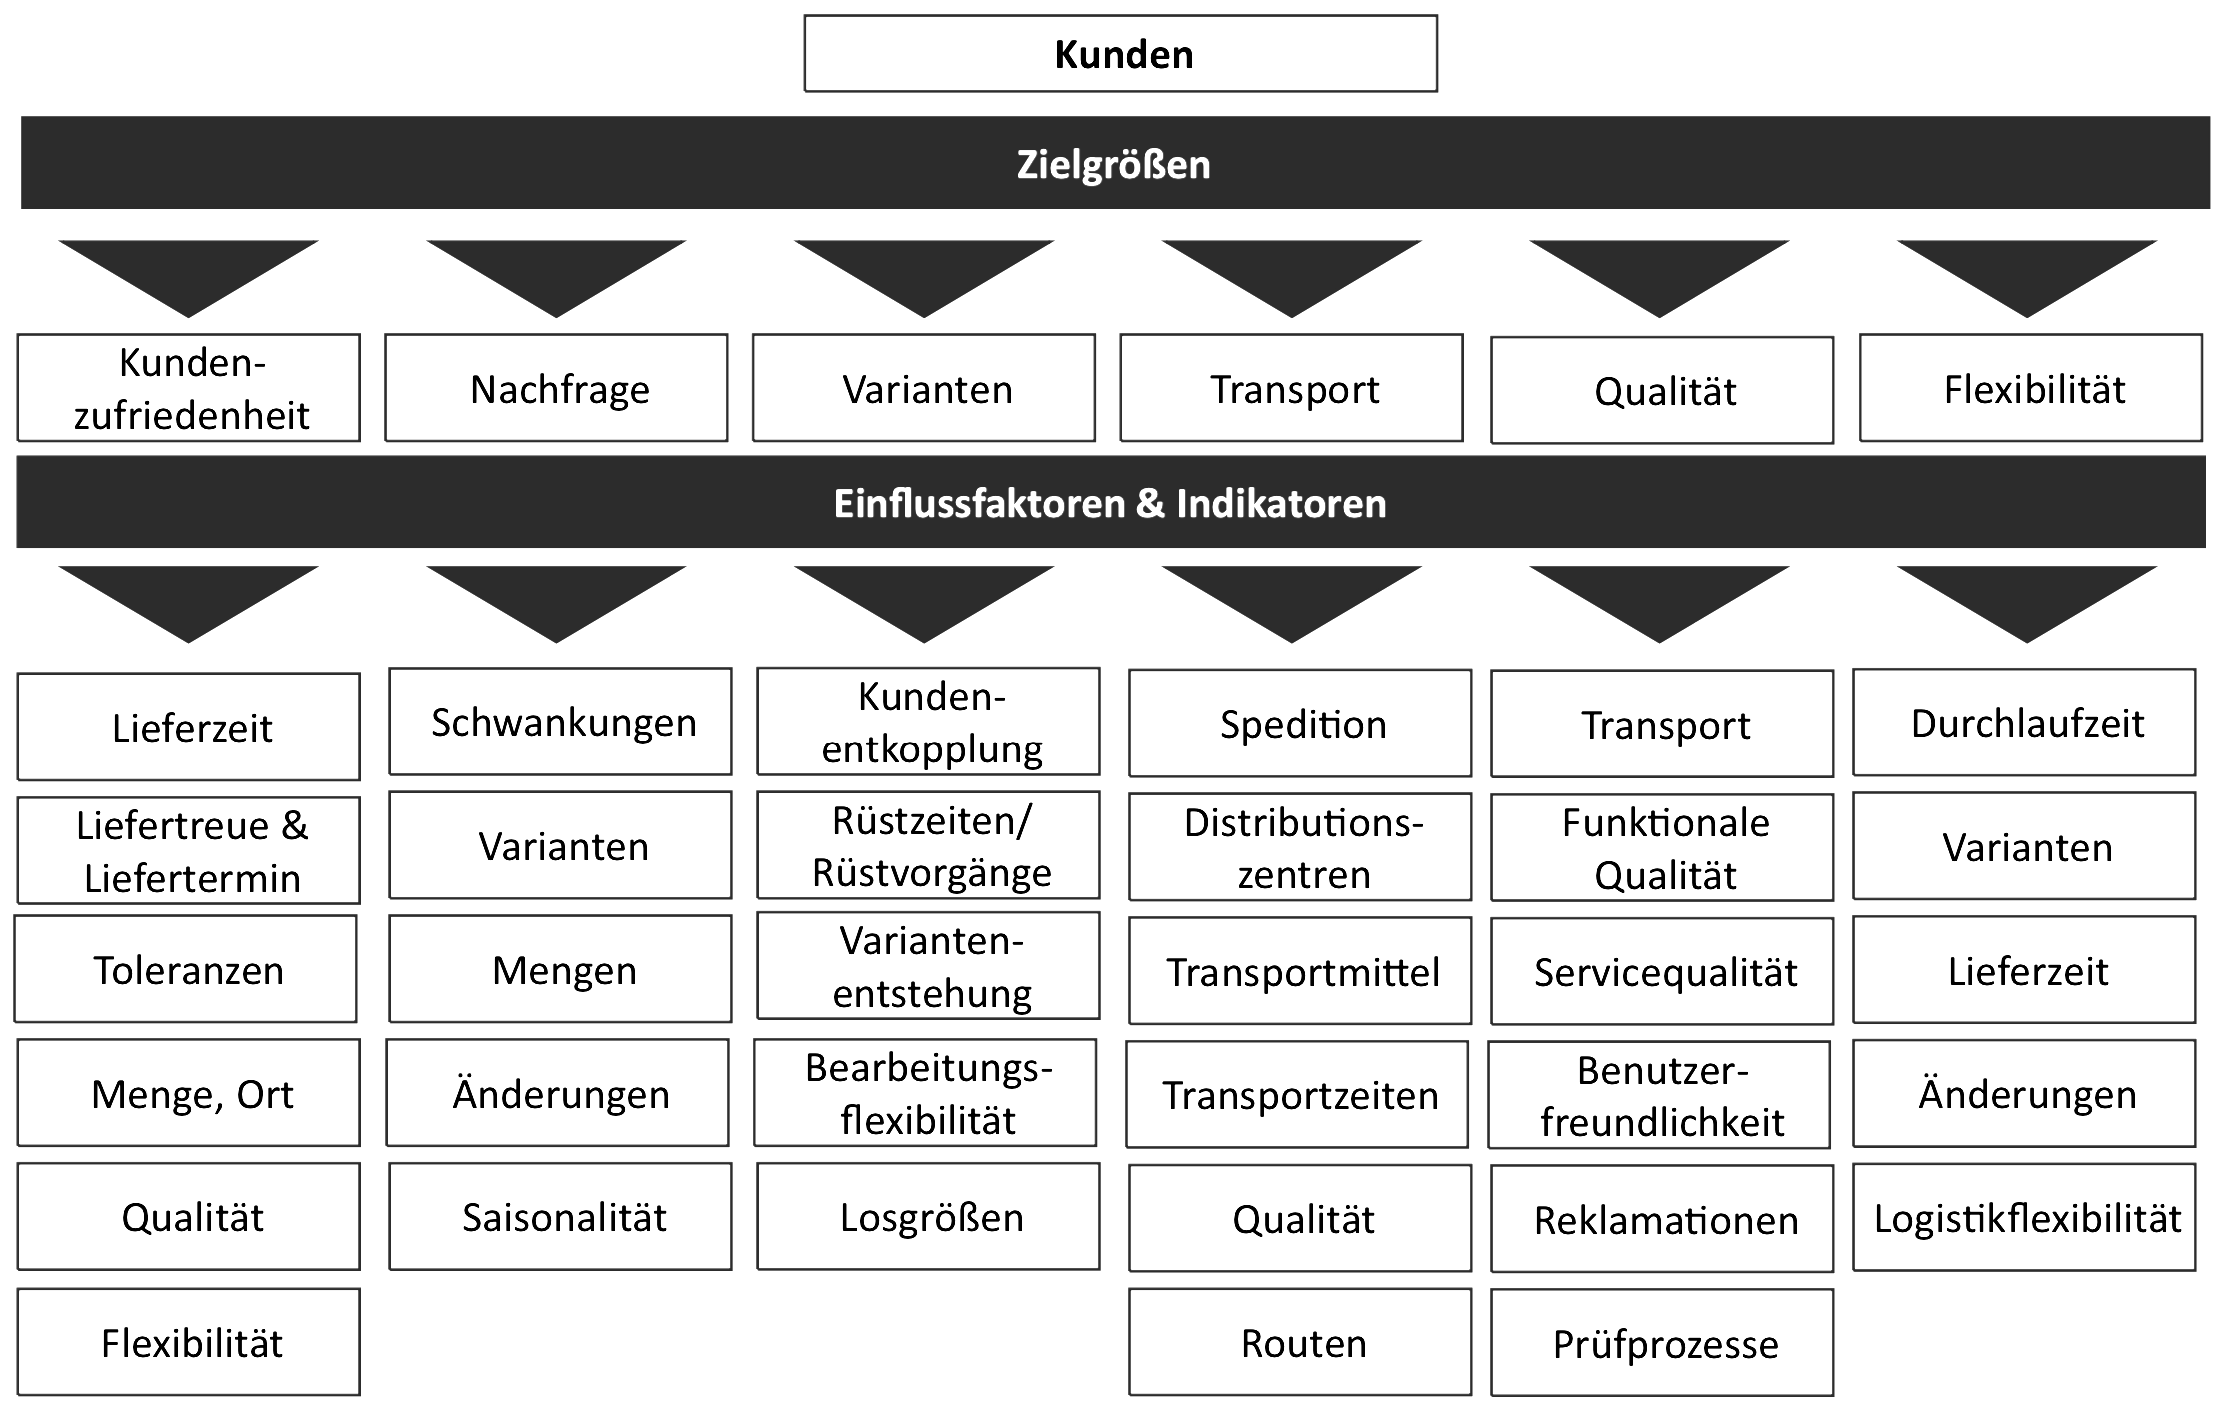
\includegraphics[width=0.8\linewidth]{gottmann_7}
	\captionof{figure}[Zielgr��en, Einflussfaktoren und Indikatoren in Richtung Kunde]{Zielgr��en, Einflussfaktoren und Indikatoren in Richtung Kunde\footnotemark}
	\label{img:gottmann_17}
	\end{figure}
	\addtocounter{footnote}{+0}\footnotetext{\cite[Abb. 3.11]{Gottmann2019}}
\section{Messmodelle zur Flexibilit�t nach Bellmann et al.}\label{b1}
%Fu�noten verteilen

%longtable
\begin{longtable}{| p{.18\textwidth} | p{.80\textwidth} |} 
\hline
\textbf{Modell von...} & \textbf{misst die} \\ \hline
\makecell[l]{Marschak/\\Nelson} & {Flexibilit�t von Entscheidungen �ber die Teilmengenbeziehung der Mengen der nach der Anfangsentscheidung noch bestehenden Handlungsm�glichkeiten\footnotemark} \\ \hline
\makecell[l]{Gupta/\\Rosenhead} & {Flexibilit�t einer Entscheidungsfolge �ber das Verh�ltnis der Anzahl der akzeptablen Endzust�nde zu der Gesamtzahl der akzeptablen Endzust�nde\footnotemark} \\ \hline
{Jacob} & {Bestandsflexibilit�tsma�zahl sowie Entwicklungsflexibilit�tsma�zahl als Quotienten des Gewinns bei optimaler Anpassung bei ,,prophetischem Wissen'' und dem Gewinn bei optimaler Anpassung entsprechend einer Entscheidung, jeweils vermindert um den Gewinn bei Nicht-Anpassung\footnotemark} \\ \hline
{Mahlmann} & {Flexibilit�t einer Entscheidung sowie Flexibilit�t des Planungsprozesses. Flexibilit�t des Planungsprozesses wird bestimmt �ber die Menge der Planrevisionszeitpunkte und Flexibilit�t der Entscheidung �ber die Anzahl von Entscheidungsm�glichkeiten, die �ber die Menge an Entscheidungsm�glichkeiten einer optimalen Strategie hinaus bestehen.\footnotemark} \\ \hline
{Hanssmann} & {Flexibilit�t einer Strategie �ber den Gesamterfolg, der damit erreicht wird. Dazu wird eine Quotient aus Gesamterfolg der Strategie und Gesamterfolg bei optimaler Anpassung, jeweils vermindert um den Gesamterfolg bei Inflexibilit�t, gebildet.\footnotemark} \\ \hline
\makecell[l]{Eversheim/\\Schaefer} & {Flexibilit�t als Kapazit�t eines Produktionssystems. Flexibilit�t wird als quantitative oder qualitative �berkapazit�t verstanden. Dementsprechend soll das Kapazit�tsangebot auf die Kapazit�tsnachfrage abgestimmt werden.\footnotemark} \\ \hline
\makecell[l]{Lassere/\\Roubellat} & {Flexibilit�t einer Entscheidung �ber das Volumen des bestehenden Handlungsraumes. Die Nebenbedingungen einer zu w�hlenden Zielfunktion (z.B. Minimierung der Lagerkosten) bilden dabei die Beschr�nkungen des Handlungsraumes. Zur Berechnung des Volumens wird ein von Laster aufgestelltes und bew�hren Theorem verwendet.\footnotemark} \\ \hline
{Kumar} & {Flexibilit�t eines Fertigungssystems �ber die Anzahl der Wahlm�glichkeiten im System (z.B. Anzahl der Aggregate oder Routen) und die Verf�gbarkeit der jeweiligen Wahlm�glichkeiten. Zur Berechnung zieht der Autor ein Entropiema� aus der Thermodynamik bzw. Informationstheorie.\footnotemark} \\ \hline
{Pauli} & {Flexibilit�t �ber Kennzahlen. So steht. bspw. das Verh�ltnis von Anzahl wirtschaftlicher Absatzregionen f�r die statische �rtliche Flexibilit�t.\footnotemark} \\ \hline
{Wolf} & {Flexibilit�t als Kapazit�t eines Produktionssystems, die in Matrizen beschrieben wird. Wenn die Kapazit�tsnachfrage gr��er als das Kapazit�tsangebot ist, besteht eine Kapazit�tsl�ckenmatrix. Interpretiert als Flexibilit�tsl�cken, ist ein System um so flexibler, desto mehr Flexibilit�tsl�cken gedeckt werden k�nnen.\footnotemark} \\ \hline
\makecell[l]{Mandelbaum/\\Buzacott} & {Flexibilit�t einer Entscheidung �ber die M�chtigkeit der Menge der Folgereaktionen. D.h., je mehr Handlungsoptionen eine Entscheidung erm�glicht, desto flexibler ist sie.\footnotemark} \\ \hline
\makecell[l]{Schneewei�/\\K�hn} & {Flexibilit�t einer Aktionenfolge �ber ein Verrichtungsma�. Das Verrichtungsma� gibt an, welche Systemzielwirkung eine Aktionenfolge besitzt, z.B. im Bezug auf Kosten, Gewinn etc. Die Flexibilit�t einer Aktionenfolge wir berechnet als Quotient aus dem Verrichtungsma� der Aktionenfolge und dem Verrichtungsma� einer optimalen Aktionsfolge bei Sicherheit �ber zuk�nftige Zust�nde, jeweils vermindert um das Verrichtungsma� einer Aktionenfolge, die keine Anpassung vorsieht.\footnotemark} \\ \hline
{Ost} & {Flexibilit�t von Maschinen �ber Kennzahlen, die f�r einen Teilflexibilit�tenkatalog bestimmt werden. Durch die Zuteilung eines Wahrheitsgrades im Rahmen einer fuzzy-logic-Berechnung erstellt der Autor eine Hierarchie von Flexibilit�tsbedarfen f�r die Teilflexibilit�ten.\footnotemark} \\ \hline
{Chen/Chung} & {Flexibilit�t flexibler Fertigungssysteme (FFS) �ber Kennzahlen in Form von Bearbeitungsflexibilit�t und Routenflexibilit�t. Die Ma�zahl f�r Bearbeitungsflexibilit�t ist der Quotient aus Anzahl der f�r ein FFS durchf�hrbaren Aufgaben und Gesamtzahl aller Aufgaben eines Produktionssystems, Routenflexibilit�t der Quotient aus der Summe aller m�glichen Wege der Werkl�cke durch ein FFS und Menge aller Werkst�cke.\footnotemark} \\ \hline
\makecell[l]{Meier-\\Barthold} & {Flexibilit�t von Probleml�sungsverfahren �ber die Menge zul�ssiger Entscheidungsfolgen eines Probleml�sungsverfahrens und M�chtigkeit der Menge der zul�ssigen Entscheidungsfolgen eines ,,best case'' bzw. den Quotient aus Volumen der Menge zul�ssiger Entscheidungsfolgen eines Probleml�sungsverfahrens und Volumen der Menge der zul�ssigen Entscheidungsfolgen eines ,,best case''.\footnotemark} \\ \hline
{Nagel} & {Flexibilit�t eines Produktionssystems �ber Flexibilit�tskosten, die durch Ressourcenmehrbedarfe entstehen. Um diese Mehrbedarfe ermitteln zu k�nnen, nutzt die Autorin den System Dynamics-Ansatz [sic!] zur Erfassung des gesamten Ressourceneinsatzes und -bedarfes.\footnotemark} \\ \hline
\makecell[l]{Corsten/\\G�ssinger} & {Flexibilit�t eines Produktionssystems f�r Dienstleistungen �ber die Berechnung der Volumina, die durch Mengen an ,,l�sbaren Problemen'' und ,,akzeptablen Probleml�sungen'' bestimmt sind. beide Mengen sind jeweils durch die Entscheidung �ber das Produktionssystem festgelegt.\footnotemark} \\ \hline
{Mirschel} & {Flexibilit�t von Produktionssystemen mit Kennzahlen. Zur Operationalisieren von Flexibilit�tspotentialen unterscheidet der Autor Teilflexibilit�ten auf drei Ebenen und nutzt bspw. Kapazit�tsdifferenzen zwischen minimaler und maximaler Kapazit�t eines Aggregates als Messgr��en.\footnotemark} \\ \hline
\makecell[l]{Realoptions-\\bewertungs-\\modelle} & {Flexibilit�t von Realoptionen. Analog Finanzoptionen erlauben es Realoptionen eine zuk�nftige Wahl zwischen zwei Zust�nden (z.B. Erweiterung oder Nicht-Erweiterung der Kapazit�t einer Anlage zu treffen, was eine Form der Flexibilit�t interpretiert wird. [sic!] Instrumente zur Finanzoptionsbewertung k�nnen dementsprechend genutzt werden, um die Flexibilit�t von Realoptionen zu messen.\footnotemark} \\ \hline
\caption[Messmodelle zur Flexibilit�t nach Bellmann et al.]{Messmodelle zur Flexibilit�t nach Bellmann et al.\footnotemark}\label{tab:b1}
\end{longtable}
\addtocounter{footnote}{-19}\footnotetext{Vgl. \cite[S.42ff]{Marschak1962} zitiert nach \cite[S.98f]{Pibernik2001}}
\addtocounter{footnote}{+1}\footnotetext{Vgl. \cite[S.B18ff]{Gupta1968}}
\addtocounter{footnote}{+1}\footnotetext{Vgl. \cite[S.322ff]{jacob1974}}	
\addtocounter{footnote}{+1}\footnotetext{Vgl. \cite[S.124ff]{Mahlmann1976}}	
\addtocounter{footnote}{+1}\footnotetext{Vgl. \cite[S.228ff]{hanssmann1978}}	
\addtocounter{footnote}{+1}\footnotetext{Vgl. \cite[S.229ff]{eversheim1980}}	
\addtocounter{footnote}{+1}\footnotetext{Vgl. \cite[S.447ff]{lasserre1985} zitiert nach \cite[S.31ff]{MeierBarthold1999}}	
\addtocounter{footnote}{+1}\footnotetext{Vgl. \cite[S.957ff]{KUMAR1987}}	
\addtocounter{footnote}{+1}\footnotetext{Vgl. \cite[S.87ff]{pauli1987}}	
\addtocounter{footnote}{+1}\footnotetext{Vgl. \cite[S.25ff]{Wolf1989}}	
\addtocounter{footnote}{+1}\footnotetext{Vgl. \cite[S.17ff]{Mandelbaum1990}}	
\addtocounter{footnote}{+1}\footnotetext{Vgl. \cite[S.380ff]{schneeweiss1990}}	
\addtocounter{footnote}{+1}\footnotetext{Vgl. \cite[S.39ff]{ost1993}}	
\addtocounter{footnote}{+1}\footnotetext{Vgl. \cite[S.397ff]{CHEN1996}}	
\addtocounter{footnote}{+1}\footnotetext{Vgl. \cite[S.51ff]{MeierBarthold1999}}	
\addtocounter{footnote}{+1}\footnotetext{Vgl. \cite[S.37ff]{Nagel2003}}	
\addtocounter{footnote}{+1}\footnotetext{Vgl. \cite[S.39ff]{Corsten2006}}
\newpage	
\addtocounter{footnote}{+1}\footnotetext{Vgl. \cite[S.104ff]{mirschel2007messung}}	
\addtocounter{footnote}{+1}\footnotetext{Vgl. \cite{trigeorgis}, \cite{bengtsson2002} und \cite{Damisch2002}}	
\addtocounter{footnote}{+1}\footnotetext{Tabelle entnommen aus \cite[S.230-233, Abbildung 2]{Bellmann2009}}	
	
	
  \end{appendix}
  
\end{document}
